\documentclass[10pt, oneside]{article}
\usepackage{amsmath, amsthm, amssymb, mathrsfs, wasysym, verbatim, bbm, color, graphics, geometry, authblk}
\usepackage{booktabs, multirow, makecell,colortbl}
\usepackage{setspace}
%\usepackage{ctex}
%\usepackage{calrsfs}
\usepackage{braket}
\usepackage{caption}
%\usepackage{subcaption}
\usepackage{subfigure}
\usepackage{hyperref}
\usepackage{framed}
\usepackage{bm}
\usepackage{tikz}
%\usepackage{mathptmx}
\hypersetup{
	colorlinks=true,
	linkcolor=blue,
	filecolor=blue,      
	urlcolor=blue,
	citecolor=blue,
}

\usetikzlibrary{shapes.geometric, arrows}
% Styles
\tikzstyle{startstop} = [ellipse, minimum width=3cm, minimum height=1cm,
                         text centered, draw=black, fill=red!30]
\tikzstyle{process}   = [rectangle, draw=black, fill=green!20,
                         minimum width=5cm, minimum height=1cm, text centered]
\tikzstyle{decision}  = [diamond, draw=black, fill=yellow!30,
                         aspect=2, text centered, inner sep=1pt]
\tikzstyle{arrow}     = [thick,->,>=stealth]

\geometry{tmargin=0.75in, bmargin=.75in, lmargin=.75in, rmargin=.75in}
\setlength{\parindent}{2em} % 设置段落首行缩进为两个汉字符
\setlength{\parskip}{1pt} % 设置段前段后距离为0
%the \bm 就是 \bm{}

\newcommand{\te}{\theta}
\newcommand{\ph}{\phi}
\newcommand{\ps}{\psi}
\newcommand{\vph}{\varphi}
\newcommand{\vps}{\varpsi}
\newcommand{\pr}{\prime}
\newcommand{\mr}[1]{\mathrm{#1}}
\newcommand{\mb}[1]{\mathbf{#1}}
\newcommand{\p}[1]{\left(#1\right)}
\newcommand{\bb}[1]{\left[#1\right]}
\newcommand{\br}[1]{\left\{#1\right\}}
\newcommand{\bv}[1]{\left|#1\right|}

\title{Continuum Model of Twisted Bilayer Graphene}
\author[1]{Qian-Sheng Shi}
\affil[1]{\textit{School of Physical Science and Technology, ShanghaiTech University, Shanghai 201210, China}}
\date{\today}

\begin{document}
	
\maketitle

\tableofcontents

\section{Band Folding}
\subsection{1D Atom Chain}
The Hamiltonian of 1D atom chain with \(N\) primitive cells which one primitive cell contains one atom(sublattice/orbital) and we only consider the nearest neighbour coupling is 
\begin{align}
    \hat{H} = -t \sum_{n = 1}^{N-1} \p{\hat{c}^{\dagger}_{x_{n+1}} \hat{c}_{x_{n}} + h.c.} ,
\end{align}
where \(x_{n} = n a\) is the position of the \(n\)th atom and \(a\) is the lattice constant. The creation and  annihilation operators in r-space can be expressed in terms of the corresponding operators in k-space whih is 
\begin{align}
    \begin{split}
        \hat{c}^{\dagger}_{x_{n}} &= \frac{1}{\sqrt{N}}\sum_{m = 1}^{N}e^{-i k_{m} x_{n}} \hat{c}^{\dagger}_{k_m}, \\
        \hat{c}_{x_{n}} &= \frac{1}{\sqrt{N}}\sum_{m = 1}^{N}e^{i k_{m} x_{n}} \hat{c}_{k_m}.
    \end{split}
\end{align}
Thus the Hamiltonian in k-space is 
\begin{align}
    \begin{split}
        \hat{H} &= -t \sum_{n = 1}^{N - 1}\bb{\p{\frac{1}{\sqrt{N}} \sum_{m = 1}^{N}e^{-i k_{m} x_{n + 1}}\hat{c}^{\dagger}_{k_{m}}} \p{\frac{1}{\sqrt{N}} \sum_{m^\prime = 1}^{N} e^{i k_{m^\prime} x_{n}}\hat{c}_{k_{m^\prime}}} +  + h.c.} \\
        & = -\frac{t}{N} \sum_{n = 1}^{N - 1}  \sum_{m = 1}^{N }  \sum_{m^\prime = 1}^{N }\bb{e^{i \p{k_{m^\prime} - k_{m}} x_{n+1}} e^{-i k_{m} a} \hat{c}^{\dagger}_{k_{m}} \hat{c}_{k_{m^\prime}} + h.c. } \\
        & = -t \sum_{m = 1}^{N } \sum_{m^\prime = 1}^{N }\p{\delta_{k_{m^\prime}, k_{m}} e^{-i k_{m} a} \hat{c}^{\dagger}_{k_{m}} \hat{c}_{k_{m^\prime}} + h.c.} \\ 
        & = -t \sum_{m = 1}^{N } \sum_{m^\prime = 1}^{N } \delta_{m^\prime, m} \p{e^{-i k_m a} + e^{i k_{m} a}}  \hat{c}^{\dagger}_{k_m} \hat{c}_{k_{m^\prime}} \\
        & = -t \sum_{m = 1}^{N } 2 \cos \p{k_{m} a} \hat{c}^{\dagger}_{k_m} \hat{c}_{k_{m}} \\
        & = \sum_{m = 1}^{N} \epsilon_{k_{m}} \hat{c}^{\dagger}_{k_m} \hat{c}_{k_{m}} \\
        & = \sum_{k_{m} \in BZ} \epsilon_{k_{m}} \hat{c}^{\dagger}_{k_m} \hat{c}_{k_{m}},
    \end{split}
\end{align}
where the last step is because the \(k_{m}\) in the first Brillouin zone is  equivalent to the \(k_m + \frac{2 \pi j}{a}\) outside the first Brillouin zone. We also diagonlize the Hamiltonian and get the Bloch state with the \(k_{m}\) wave vector which is 
\begin{align}
    \ket{k_{m}} = \hat{c}^{\dagger}_{k_{m}} \ket{0} = \frac{1}{\sqrt{N}} \sum_{n = 1}^{N} e^{i k_{m} x_{n}} \ket{x_{n}},
\end{align} 
and the dispersion relation is 
\begin{align}
    \epsilon_{k_{m}} = -2t \cos \p{k_{m} a}, \quad k_{m} \in BZ = \left[0 , \frac{2\pi}{a} \right).
\end{align}


\subsection{Biparticle model}
Now we choose two atoms as one primitive cell thus there is \(N/2\) primitive cells in the chain. We use \(\p{j, \alpha}\) to label the \(\alpha\)th atom(sublattice) in the \(j\)th primitive cell where  \(j \in \br{0,\cdots, N/2 - 1} \) and \(\alpha \in \br{0, 1}\). Thus
\begin{align}
	x_{j, \alpha} = 2 j a + \alpha a = \p{2j + \alpha}a = x_{n = 2j + \alpha},
\end{align}
and the new creation operators are
\begin{align}
	\hat{d}^{\dagger}_{j, \alpha} = \hat{c}^{\dagger}_{x_{2j + \alpha}}.
\end{align}
The Hamiltonian is 
\begin{align}
	\hat{H} = -t \sum_{j = 1}^{N/2 - 1} \p{\hat{d}^{\dagger}_{j,1}\hat{d}_{j,0} + h.c.} + \p{\hat{d}^{\dagger}_{j,0}\hat{d}_{j - 1,1} + h.c.},
\end{align}
and the new creation and annihilation operators in r-space can be expressed in terms of the corresponding operators in k-space which is
\begin{align}
	\begin{split}
		\hat{d}^{\dagger}_{j, \alpha} &= \frac{1}{\sqrt{N/2}} \sum_{m = 1}^{N/2} e^{-i k_{m} x_{j, \alpha}} \hat{d}^{\dagger}_{k_{m}},\\
	\hat{d}_{j, \alpha} &= \frac{1}{\sqrt{N/2}} \sum_{m = 1}^{N/2} e^{i k_{m} x_{j, \alpha}} \hat{d}_{k_{m}}.
	\end{split}
\end{align}
where \(k_{m} = \frac{2\pi m}{N/2 a} , m \in \br{1, \cdots, N/2}\) and the mini Brillouin zone is 
\begin{align}
	k_{m} \in mBZ = \left[0,\pi/a \right),
\end{align}
The Hamiltonian in k-space is 
\begin{align}
	\begin{split}
		\hat{H} & = -t \sum_{j = 1}^{N/2 - 1} \p{\hat{d}^{\dagger}_{j,1}\hat{d}_{j,0} + h.c.} + \p{\hat{d}^{\dagger}_{j,0}\hat{d}_{j - 1,1} + h.c.}  \\
		& = -t \sum_{j = 1}^{N/2 - 1} \bb{ \p{\frac{1}{\sqrt{N/2}} \sum_{m = 1}^{N/2} e^{-i k_{m} x_{j,1}} \hat{d}^{\dagger}_{k_{m}, 1}}\p{\frac{1}{\sqrt{N/2}} \sum_{m^\prime = 1}^{N/2} e^{i k_{m^\prime} x_{j,0}} \hat{d}_{k_{m^\prime},0} } + h.c.} \\
		& \quad + \bb{\p{\frac{1}{\sqrt{N/2}} \sum_{m = 1}^{N/2} e^{- k_{m} x_{j,0} }\hat{d}^{\dagger}_{k_m, 0} } \p{\frac{1}{\sqrt{N/2}} \sum_{m^\prime = 1}^{N/2} e^{i k_{m^\prime} x_{j-1, 1}} \hat{d}_{k_{m^\prime}, 1}} + h.c.} \\
		& = -t  \sum_{m = 1}^{N/2} \sum_{m^\prime = 1}^{N/2} \delta_{m, m^\prime} \p{e^{-i k_{m} a} \hat{d}^{\dagger}_{k_{m}, 1} \hat{d}_{k_{m}, 0} + h.c.} + \delta_{m, m^\prime} \p{e^{-i k_{m} a} \hat{d}^{\dagger}_{k_{m}, 0} \hat{d}_{k_{m}, 1} + h.c.} \\
		& = \sum_{k_{m} \in mBZ} \begin{pmatrix}
			\hat{d}^{\dagger}_{k_{m}, 0} & \hat{d}^{\dagger}_{k_{m}, 1}
		\end{pmatrix}
		\begin{pmatrix}
			0 & -2t \cos\p{k_{m} a} \\
			-2t \cos\p{k_{m} a} & 0
		\end{pmatrix}
		\begin{pmatrix}
			\hat{d}_{k_{m}, 0} \\ \hat{d}_{k_{m}, 1}
		\end{pmatrix} \\
		& =  \sum_{k_{m} \in mBZ} \hat{d}^{\dagger}_{k_{m}} H\p{k_m} \hat{d}_{k_{m}}.
	\end{split}
\end{align}
So it's a \(2 \times 2\) Bloch Hamiltonian and every k-point has an extra 2 degree of freedom from sublattice. We can diagonlize the Bloch Hamiltonian with a unitary transformation \(\hat{\gamma} = U  \hat{d}\) and the Hamiltonian changes into 
\begin{align}
	\hat{H} = \sum_{k_{m} \in mBZ} \hat{\gamma}^{\dagger}_{k_m} U \p{k_{m}} H \p{k_m} U^{\dagger} \p{k_m} \hat{\gamma}_{k_m} = \sum_{k_{m} \in mBZ} \hat{\gamma}^{\dagger}_{k_m} D \hat{\gamma}_{k_m}l,
\end{align}
where we add the sublattice index to express \(\hat{\gamma}\)
\begin{align}
	\hat{\gamma}_{k_m, \alpha^\prime} = \sum_{\alpha} U_{\alpha^\prime \alpha} \p{k_m} \hat{d}_{k_m, \alpha}.
\end{align}
So the unitary matrix
\begin{align}
	U  = \begin{pmatrix}
		1/\sqrt{2} & 1/\sqrt{2} \\
		1/\sqrt{2} & -1/\sqrt{2}
	\end{pmatrix}
\end{align}
and the diagonal matrix is 
\begin{align}
	D = \begin{pmatrix}
		-2t \cos\p{k_m a} & 0 \\ 
		0 & 2t \cos\p{k_m a}
	\end{pmatrix}.
\end{align}
Thus the eigenvalue is \(\epsilon_{\pm} \p{k_m} = \pm 2t \cos \p{k_m a}\) and \(\hat{\gamma}_{k_{m}, \pm} = \frac{1}{\sqrt{2}} \p{\hat{d}_{k_{m}, 0} \pm \hat{d}_{k_{m}, 1}}\). More specifically
\begin{align}
	\begin{split}
		\hat{\gamma}_{k_m, +} & = \frac{1}{\sqrt{2}} \p{\hat{d}_{k_{m}, 0} + \hat{d}_{k_{m}, 1}} \\
		& = \frac{1}{\sqrt{2}} \frac{1}{\sqrt{N/2}} \sum_{j = 0}^{N/2 - 1}\p{e^{- i k_{m} x_{j, 0}} \hat{d}_{j, 0}  + e^{-i k_{m} x_{j, 1}} \hat{d}_{j,1}} \\
		& = \frac{1}{\sqrt{N}} \sum_{n = 0}^{N - 1} e^{-i k_{m} x_{n}} \hat{c}_{n} \\
		& = \hat{c}_{k_{m}},
	\end{split}
\end{align}
and 
\begin{align}
	\begin{split}
		\hat{\gamma}_{k_m, -} & = \frac{1}{\sqrt{2}} \p{\hat{d}_{k_{m}, 0} - \hat{d}_{k_{m}, 1}} \\
		& = \frac{1}{\sqrt{2}} \frac{1}{\sqrt{N/2}} \sum_{j = 0}^{N/2 - 1}\p{e^{- i k_{m} x_{j, 0}} \hat{d}_{j, 0} - e^{-i k_{m} x_{j, 1}} \hat{d}_{j,1}} \\
		& = \frac{1}{\sqrt{N}} \sum_{n = 0}^{N/2 - 1} \p{e^{-i k_m 2j a  + i 2j \pi} \hat{c}_{x_{2j}} + e^{-i k_{m} \p{2j+1} a + i \p{2j + 1} \pi} \hat{c}_{x_{2j + 1}}} \\
		& = \frac{1}{\sqrt{N}} \sum_{n = 0}^{N/2 - 1} \p{e^{-i \p{k_{m} + \pi/a} x_{2j}} \hat{c}_{x_{2j}} + e^{-i \p{k_{m} + \pi/a} x_{2j + 1}} \hat{c}_{x_{2j + 1}} } \\
		& = \hat{c}_{k_{m} + \pi/a},
	\end{split}
\end{align}
where the new reciprocal lattice basis vector is \(b^{m} = \pi/a\). So the original Brillouin Zone can be divided into mBZ and mBZ\(+ b^{m}\) where \(m\) represent for mini of moiré. The Hamiltonian  of the whole 1D-atom chain can be rewriten as
\begin{align}
	\begin{split}
		\hat{H} & = \sum_{k_m \in BZ} \epsilon\p{k_{m}} \hat{c}^{\dagger}_{k_m} \hat{c}_{k_m} \\
		& = \sum_{k_m \in mBZ} \begin{pmatrix}
			\hat{c}^{\dagger}_{k_m} & \hat{c}^{\dagger}_{k_m + b^m}
		\end{pmatrix} \begin{pmatrix}
			\epsilon\p{k_{m}} & \\
			  &  \epsilon\p{k_{m} + b^m}
		\end{pmatrix} \begin{pmatrix}
			\hat{c}^{\dagger}_{k_m} \\ \hat{c}^{\dagger}_{k_m + b^m}
		\end{pmatrix}.
	\end{split}
\end{align}
For different reciprocal lattice basis vector like \(\bm{b}^{m}_{1}\) and  \(\bm{b}^{m}_{2}\), we can construct the wave vector like \(\bm{k} + n_{1} \bm{b}^{m}_{1} + n_2 \bm{b}^{m}_{2}\) where the dispersion relation is same for each \(\hat{c}^{\dagger}_{\bm{k} + n_{1} \bm{b}^{m}_{1} + n_2 \bm{b}^{m}_{2}}\) and \(\hat{c}_{\bm{k} + n_{1} \bm{b}^{m}_{1} + n_2 \bm{b}^{m}_{2}}\).


\subsection{Flat Band}
Due to the scattering at the boundary of the Brillouin Zone, there is a gap in the energyband. As the effect of band folding becomes stronger, the two bands corresponding to the gap become increasingly flatter



\section{Dirac Cone}
\subsection{Geometry of Graphene}
The basis vectors of monolayer are 
\begin{align}
	\bm{a}_{1} = a\p{\frac{1}{2}, \frac{\sqrt{3}}{2}} ,\quad \bm{a}_{2} &= a\p{-\frac{1}{2}, \frac{\sqrt{3}}{2}},
\end{align}
where \(a = \sqrt{3} d\) is the lattice constant of graphene and \(d = 1.42\) \AA  which is the carbon-carbon distance. The positions of two sublattices are
\begin{align}
	\bm{\tau}_{A} = \p{0, 0} , \quad \bm{\tau}_{B} = \p{0, \frac{a}{\sqrt{3}}}.
\end{align}
The correspondingly reciprocal lattice basis vectors are 
\begin{align}
	\bm{b}_{1} = \frac{4 \pi}{\sqrt{3} a} \p{\frac{\sqrt{3}}{2}, \frac{1}{2}}, \quad  \bm{b}_{2} = \frac{4 \pi}{\sqrt{3} a} \p{-\frac{\sqrt{3}}{2}, \frac{1}{2}}.
\end{align}
and the position of Dirac points are  
\begin{align}
	\bm{K} = \frac{4 \pi}{3 a}\p{1, 0}, \quad \bm{K}^{\prime} = \frac{4 \pi}{3 a}\p{-1, 0}.
\end{align} 
The Hamiltonian of graphene in tight-binding model is 
\begin{align}
	H = -t \sum_{\bm{k}} \begin{pmatrix}
		\hat{a}^{\dagger}_{\bm{k}} & \hat{b}^{\dagger}_{\bm{k}}
	   \end{pmatrix}\begin{pmatrix}
	   0 & 1+ e^{-i \bm{k} \cdot \bm{a}_{1}} + e^{-i \bm{k} \cdot \bm{a}_{2}} \\ 
	   1+ e^{i \bm{k} \cdot \bm{a}_{1}} + e^{i \bm{k} \cdot \bm{a}_{2}} & 0
	   \end{pmatrix} \begin{pmatrix}
	   \hat{a}_{\bm{k}} \\ \hat{b}_{\bm{k}}
	   \end{pmatrix},
\end{align}
where \(t = 2.7 \mr{eV}\)  and the Bloch Hamiltonian defined as 
\begin{align}
	h\left(\bm{k}\right) = - t\begin{pmatrix}
		0 & 1+ e^{-i \bm{k} \cdot \bm{a}_{1}} + e^{-i \bm{k} \cdot \bm{a}_{2}} \\ 
		1+ e^{i \bm{k} \cdot \bm{a}_{1}} + e^{i \bm{k} \cdot \bm{a}_{2}} & 0
	\end{pmatrix},
\end{align}
and 
\begin{align}
	f\left( \bm{k} \right) = 1+ e^{-i \bm{k} \cdot \bm{a}_{1}} + e^{-i \bm{k} \cdot \bm{a}_{2}}.
\end{align}
The Bloch Hamiltonian can be expanded around \(\bm{K}\) as 
\begin{align}
	\begin{split}
		h\p{\bm{p}}\left. \bigg| \right._{\bm{p} \rightarrow \bm{K}} & = \frac{\sqrt{3} a t}{2} \begin{pmatrix}
			0 & k_{x} - i k{y} \\
			k_{x} + i k_{y} & 0
		\end{pmatrix} \\
		& = v_{F} \hbar |\bm{k}| \begin{pmatrix}
			0 & e^{-i \te_{\bm{k}}} \\
			e^{i \te_{\bm{k}}} & 0
		\end{pmatrix} \\
		& = v_{F} \, \hat{\bm{p}_{\bm{k}}} \cdot \hat{\sigma}.
	\end{split}
\end{align}
where \(V_{F} =  \frac{\sqrt{3} a t}{2 \hbar}\) is the Fermi velocity and \(\bm{p}_{\bm{k}} = \hbar \bm{k}\) is the momentum of wave vector \(\bm{k}\).

\subsection{Berry phase of Dirac cone}
Since the Hamiltonian Hamiltonian around Dirac point can be expressed as \(H = v_{F} \bm{\sigma} \cdot \bm{k}\) where we suppress the \(\hbar\) for convenience. So the eigenequation is 
\begin{align}
	v_{F} \bv{\bm{k}}
	\begin{pmatrix}
		0 & e^{-i \te} \\
		e^{i \te} & 0 
	\end{pmatrix} \ket{\psi} = E \ket{\psi} 
\end{align}
where \(\te\) is the argument of \(\bm{k}\). For the upper band(conduction band), its eigenvalue is \(E_{+} = v_{F} \bv{\bm{k}}\). Plugging it into the eigenequation, we can get the eigenstate
\begin{align}
	\ket{\psi_{+}} = \frac{1}{\sqrt{2}} \begin{pmatrix}
		1 \\
		e^{i \te}
	\end{pmatrix}.
\end{align}
The definition of Berry phase \(\gamma\) is 
\begin{align}
	\gamma = \oint_{\mathcal{{C}}} d \bm{k} \bm{A} \p{\bm{k}} = \int d \bm{S} \cdot \bm{S} \p{\bm{k}},
\end{align}
where \(\bm{A}\) is the Berry connection and \(\bm{S}\) is the Berry curature, \(\bm{k}\) is the parameter space and \(\mathcal{C}\) is a close loop in the parameter space. In this case, the Berry connection is
\begin{align}
	\begin{split}
		\bm{A} \p{\phi} & = i \braket{\psi \p{\te} | \partial_{\te} | \psi \p{\te}} \\
		& = i \frac{1}{2} \begin{pmatrix}
			1 & e^{-i \te}
		\end{pmatrix} \begin{pmatrix}
			0 \\
			i e^{i \te}
		\end{pmatrix} \\
		& = -\frac{1}{2}.
	\end{split} 
\end{align}
So the Berry phase is
\begin{align}
	\gamma = \oint_{\mathcal{C}} d \te \, A \p{\te} = \int_{0}^{2 \pi} d \te \, \p{-\frac{1}{2}} = - \pi.
\end{align}	

We say the Berry phase around Dirac point is \(-\pi\). Similarly, we can get the Berry phase around \(\bm{K}^{\prime}\) point is \(+\pi\). It like the spin half system where it takes two circles to return to the original state, which we called it as pseudospin. But actually it is the sublattice degree of freedom which means there is a phase difference between the wavefunction on two sublattices when an electron move around the Dirac point.


\subsection{Rotated Dirac Cone}
The basis vectors after the counterclockwise rortation are 
\begin{align}
	\bm{a}^{\te} = M\p{\te} \bm{a},
\end{align}
where 
\begin{align}
	M\p{\te} = \begin{pmatrix}
		\cos \te & -\sin \te \\
		\sin \te & \cos \te 
	\end{pmatrix}.
\end{align}
Thus 
\begin{align}
	\begin{split}
		\bm{a}^{\te}_{1} &= a \p{\frac{1}{2} \cos\te -\frac{\sqrt{3}}{2} \sin \te,\, \frac{1}{2} \sin \te + \frac{\sqrt{3}}{2} \cos \te} = \p{\cos \p{\frac{\pi}{3} + \te }, \sin \p{\frac{\pi}{3} + \te }}\\ \quad \bm{a}^{\te}_{2} &= a \p{-\frac{1}{2} \cos\te -\frac{\sqrt{3}}{2} \sin \te,\, -\frac{1}{2} \sin \te + \frac{\sqrt{3}}{2} \cos \te } = \p{\cos \p{\frac{2\pi}{3} + \te }, \sin \p{\frac{2\pi}{3} + \te }},
	\end{split}
\end{align}
and the basis vectors for reciprocal lattice after rotation are 
\begin{align}
	\bm{b}^{\te}_{1} = 2 \pi \frac{ \bm{a}^{\te}_{2} \times \hat{z}}{ \bm{a}^{\te}_{1} \cdot \p{\bm{a}^{\te}_{2} \times \hat{z}}},\quad \bm{b}^{\te}_{2} = 2 \pi \frac{\hat{z} \times \bm{a}^{\te}_{1}}{ \bm{a}^{\te}_{1} \cdot \p{\bm{a}^{\te}_{2} \times \hat{z}}},
\end{align}
where \(\bm{a}^{\te}_{1} \cdot \p{\bm{a}^{\te}_{2} \times \hat{z}} = \frac{\sqrt{3} a^{2}}{2}\) is the volume or the square of the primitive cell which leads to 
\begin{align}
	\begin{split}
		\bm{b}^{\te}_{1} &= \frac{4 \pi}{\sqrt{3} a}\p{-\frac{1}{2} \sin \te + \frac{\sqrt{3}}{2} \cos \te, \, \frac{1}{2} \cos \te + \frac{\sqrt{3}}{2} \sin ]\te} = \frac{4 \pi}{\sqrt{3} a} \p{\cos\p{\frac{\pi}{6} + \te}, \sin\p{\frac{\pi}{6} + \te}} \\
		\bm{b}^{\te}_{2} &= \frac{4 \pi}{\sqrt{3} a}\p{-\frac{1}{2} \sin \te - \frac{\sqrt{3}}{2} \cos \te, \, \frac{1}{2} \cos \te - \frac{\sqrt{3}}{2} \sin ]\te} = \frac{4 \pi}{\sqrt{3} a} \p{\cos\p{\frac{5\pi}{6} + \te}, \sin\p{\frac{5\pi}{6} + \te}}
	\end{split}
\end{align}
The reciprocal lattice vectors rotate counterclockwise by the same angle as the basis vectors. 

So the Dirac point $\bm{K}$ after rotation is 
\begin{align}
	\bm{K}^{\te} = M\p{\te} \bm{K} = \frac{4 \pi}{3 a} \begin{pmatrix}
		\cos \te & -\sin \te \\
		\sin \te & \cos \te 
	\end{pmatrix} \begin{pmatrix}
		1 \\ 0 
	\end{pmatrix} =  \frac{4 \pi}{3 a} \begin{pmatrix}
		\cos \te \\ \sin \te 
	\end{pmatrix} =  \frac{4 \pi}{3 a} \p{\cos \te, \sin \te}.
\end{align}
Now the \(f\p{\bm{p}}\) changes into 
\begin{align}
	f^{\te} \p{\bm{p}} = 1 + e^{-i \bm{p} \cdot \bm{a}^{\te}_{1}}+ e^{-i \bm{p} \cdot \bm{a}^{\te}_{2}},
\end{align}
and we expand it around \(\bm{K}^{\te}\) 
\begin{align}
	f^{\te}\p{\bm{p}} = f^{\te}\p{\bm{K}^{\te}} + \frac{\partial f^{\te} \p{\bm{p}}}{\partial p_{x} }\left. \bigg| \right._{\bm{p} \rightarrow \bm{K}^{\te}} \p{p_{x} - K^{\te}_{x}} + \frac{\partial f^{\te}\p{\bm{p}}}{\partial p_{y} }\left. \bigg| \right._{\bm{p} \rightarrow \bm{K}^{\te}} \p{p_{y} - K^{\te}_y} + o\p{\bm{p}^{2}},
\end{align}
where \(\bm{p} = \bm{K}^{\te} + \bm{k}\). The derivatives are 
\begin{align}
	\begin{split}
		\frac{\partial f^{\te} \p{\bm{p}}}{\partial p_{x} }\left. \bigg| \right._{\bm{p} \rightarrow \bm{K}^{\te}} & = \frac{\partial}{\partial p_{x}} \br{1 + e^{-i a\bb{p_{x} \cos \p{\frac{\pi}{3} + \te}+ p_{y} \sin \p{\frac{\pi}{3} + \te}} }+ e^{-i a\bb{p_{x} \cos \p{\frac{2\pi}{3} + \te}+ p_{y} \sin \p{\frac{2\pi}{3} + \te}} }}\left. \bigg| \right._{\bm{p} \rightarrow \bm{K}^{\te}} \\
		& = -ia \br{\cos \p{\frac{\pi}{3} + \te} e^{-i a\bb{p_{x} \cos \p{\frac{\pi}{3} + \te}+ p_{y} \sin \p{\frac{\pi}{3} + \te}} } + \cos \p{\frac{2\pi}{3} + \te} e^{-i a\bb{p_{x} \cos \p{\frac{2\pi}{3} + \te}+ p_{y} \sin \p{\frac{2\pi}{3} + \te}} } }\left. \bigg| \right._{\bm{p} \rightarrow \bm{K}^{\te}} \\
		& = -ia \p{\cos \p{\frac{\pi}{3} + \te} e^{-i\frac{2\pi}{3}} + \cos \p{\frac{2\pi}{3} + \te} e^{i\frac{2\pi}{3}}} \\
		& = -i a \br{-\frac{1}{2} \bb{\cos \p{\frac{\pi}{3} + \te} + \cos \p{\frac{2\pi}{3} + \te}} + \frac{\sqrt{3}}{2}i \bb{\cos \p{\frac{2\pi}{3} + \te} - \cos \p{\frac{\pi}{3} + \te}}} \\
		& = \frac{\sqrt{3}}{2}a\p{-\cos \te - i\sin \te},
	\end{split}
\end{align}
Similarily
\begin{align}
		\frac{\partial f^{\te} \p{\bm{p}}}{\partial p_{y} }\left. \bigg| \right._{\bm{p} \rightarrow \bm{K}^{\te}} & = \frac{\sqrt{3}}{2}a\p{- \sin \te + i \cos \te}.
\end{align}
So 
\begin{align}
	f^{\te} \p{\bm{p}} \left. \bigg| \right._{\bm{p} \rightarrow \bm{K}^{\te}}= \frac{\sqrt{3}}{2}a\bb{\p{-\cos \te-i \sin\te} k_{x} + \p{-\sin \te + i \cos \te} k_{y}},
\end{align}
and the Bloch Hamiltonian changes into 
\begin{align}
	\begin{split}
		h^{\p{\te}} \p{\bm{p}}\left. \bigg| \right._{\bm{p} \rightarrow \bm{K}^{\te}}& = -t \begin{pmatrix}
			0 & f^{\te} \\
			\p{f^{\te}}^{*} & 0
		\end{pmatrix}\\
		& = -t \begin{pmatrix}
			0 & \frac{\sqrt{3} a}{2} \bb{\p{-\cos \te -i \sin \te} k_{x} + \p{- \sin \te + i \cos \te} k_{y}} \\
			\frac{\sqrt{3} a}{2} \bb{\p{-\cos \te +i \sin \te} k_{x} + \p{- \sin \te - i \cos \te} k_y}  & 0
		\end{pmatrix} \\
		& = \frac{\sqrt{3} a t}{2 \hbar} \hbar |\bm{k}| \begin{pmatrix}
			0 & \cos \p{\te - \te_{\bm{k}}} + i  \sin \p{\te - \te_{\bm{k}}} \\
			\cos \p{\te - \te_{\bm{k}}} - i  \sin \p{\te - \te_{\bm{k}}}  & 0 
		\end{pmatrix} \\
		& = v_F \hbar  |\bm{k}| \begin{pmatrix}
			0 & e^{i \p{\te - \te_{\bm{k}}}} \\
			e^{ - i \p{\te - \te_{\bm{k}}}} & 0
		\end{pmatrix}  \\ 
		& = v_F \hbar  |\bm{k}| \begin{pmatrix}
			0 & e^{ -i \p{\te_{\bm{k}} - \te}} \\
			e^{i \p{\te_{\bm{k}} - \te}} & 0
		\end{pmatrix}.
	\end{split}
\end{align}
If the rotation is clockwise, the Bloch Hamiltonian changes into with the $\te \rightarrow - \te$
\begin{align}
	h^{\p{\te}} \p{\bm{p}}\left. \bigg| \right._{\bm{p} \rightarrow \bm{K}^{\te}} = v_F \hbar  |\bm{k}| \begin{pmatrix}
		0 & e^{-i \p{\te + \te_{\bm{k}}}} \\
		e^{  i \p{\te + \te_{\bm{k}}}} & 0
	\end{pmatrix}.
\end{align}

\begin{framed}
We need to point out that it is actually a passive rotation. That is, we defined active rotation as rotating the coordinate axes while keeping the physical system fixed. But in the preview derivation, we actually rotated the lattice basis vectors  actively or counterclockwisly rotated the basis vectors \(\te/2\). \\

So the fixed momentum \(\bm{k}\) appears to have shifed in the opposite direction(clockwisely) or passive rotation.
\end{framed}

\begin{itemize}
	\item Another Two Ways
\end{itemize}

For the spinor representation, where 
\begin{align}
	\hat{\sigma}^{\te} = U\p{\te} \hat{\sigma} U^{\dagger} \p{\te},
\end{align}
where the standard active rotation operator for spin-\(\frac{1}{2}\) particles is
\begin{align}
	U\p{\theta} = \exp\p{-i \frac{\hat{J}_{z}}{\hbar} \theta} = \exp\p{-i \frac{\theta}{2} \sigma_{z}},
\end{align}
but for the passive rotation, it should be
\begin{align}
	U\p{\te} = \exp\p{i \frac{\te}{2} \sigma_{z}} = \cos\frac{\theta}{2}I_{2\times2}+ i\sin\frac{\theta}{2}\sigma_z,
\end{align}
and
\begin{align}
	\exp\left(i\frac{\theta}{2}\sigma_z\right)\sigma_{x} \exp\left(-i\frac{\theta}{2}\sigma_z\right) &= \cos \theta \sigma_x - \sin \theta \sigma_y \\
	\exp\left(i\frac{\theta}{2}\sigma_z\right)\sigma_{y} \exp\left(-i\frac{\theta}{2}\sigma_z\right) &= \sin \theta \sigma_x +  \cos \theta \sigma_y.
\end{align}
So the Bloch Hamiltonian after rortation is 
\begin{align}
	\begin{split}
		h^{\te} \p{\bm{k}} 
		& = v_F \hbar |\bm{k}| \begin{pmatrix}
			0 & \cos \p{\te_{\bm{k}} - \te} - i \sin \p{\te_{\bm{k}} - \te} \\
			\cos \p{\te_{\bm{k}} - \te} + i \sin \p{\te_{\bm{k}} - \te} & 0
		\end{pmatrix} \\
		& = v_F \hbar |\bm{k}| \begin{pmatrix}
			0 & e^{-i \p{\te_{\bm{k}} - \te}} \\
			e^{i \p{\te_{\bm{k}} - \te}} & 0
		\end{pmatrix} \\
		& = v_F \hbar \bm{k} \cdot \sigma^{\te} .
	\end{split}
\end{align}

For the clockwise rotation along $\hat{z}$ axis with the angle of $\theta$, one of its representation matrix is 
\begin{align}
	R_{z} \p{\te} = \begin{pmatrix}
		e^{i \frac{\te}{2}} & 0 \\
		0 & e^{ - i \frac{\te}{2}}
	\end{pmatrix}.
\end{align}
The Bloch Hamiltonian after rotation can be written as
\begin{align}
	\begin{split}
		h^{\te} \p{\bm{k}} &= R_{z} \p{\te} h \p{\bm{k}} R^{-1}_{z} \p{\te} \\
		& = v_F \hbar |\bm{k}| \begin{pmatrix}
			e^{i \frac{\te}{2}} & 0 \\
			0 & e^{ - i \frac{\te}{2}}
		\end{pmatrix} \begin{pmatrix}
			0 & e^{-i \te_{\bm{k}}} \\
			e^{i \te_{\bm{k}}} & 0
		\end{pmatrix}  \begin{pmatrix}
		e^{-i \frac{\te}{2}} & 0 \\
		0 & e^{ i \frac{\te}{2}}
	\end{pmatrix} \\
	& =  v_F \hbar |\bm{k}| \begin{pmatrix}
		0 & e^{i \p{\te - \te_{\bm{k}}}} \\
		e^{ - i \p{\te - \te_{\bm{k}}}} & 0
	\end{pmatrix}.
	\end{split}
\end{align}

\section{Twisted Bilayer Graphene}
\subsection{Convention}
Assuming the AA stacking as the aligned configuration and the translation vector \(\bm{d}\) = 0. The postions of the carbon atoms in the two misaligned layers labeled by \(\bm{r}\) and \(\bm{r}^\theta\) are ralated by 
\begin{align}
	\bm{r}^\theta = M\p{\theta} \bm{r} ,
\end{align}
and 
\begin{align}
	\bm{r} = \bm{R} + \bm{\tau},
\end{align}
which leads to 
\begin{align}
	\bm{R}^{\te} = M\p{\te} \bm{R},\quad \bm{\tau}^{\te}_{\alpha} = M \p{\te} \bm{\tau}_{\alpha}, \quad \alpha \in \br{A,\, B}
\end{align}
Since the reciprocal space takes the same rotation and the reciprocal lattice \(\bm{G}^{\te} =M\p{\te} \bm{G}\), thus 
\begin{align}
	\bm{G}^{\te} \cdot \bm{R}^{\te} = \bm{G} \cdot \bm{R}, \quad \bm{G}^{\te} \cdot \bm{\tau}^{\te}_{\alpha} = \bm{G} \cdot \bm{\tau}_{\alpha}, \quad \alpha \in \br{A ,\, B}.
\end{align}
For AB stacking 
\begin{align}
	\bm{G}^{\te} \cdot \bm{\tau}^{\te}_{\alpha} = \bm{G} \cdot \p{\bm{\tau}_{\alpha} - \bm{\tau}_{B}}, \quad \alpha \in \br{A,\, B}.
\end{align}

\begin{itemize}
	\item Reciprocal Basis Vectors
\end{itemize}
In the third convention, the reciprocal basis vectors in the twised layer are \(\bm{b}^{\te}_{l} = M \p{\te} \bm{b}_{l}\) where the \(l\) is the index of layer. So we can choose a periodic function 
\begin{align}
	h_{l} \p{\bm{r}} = \sum_{i = 1}^{3} \cos \p{\bm{G}_{l,i} \cdot \bm{r}},
\end{align}
where we defined \(\bm{G}_{l,1} = \bm{b}_{l,1}, \,\bm{G}_{l,2} = \bm{b}_{l,2}, \, \bm{G}_{l,3} = \bm{b}_{l,1} - \bm{b}_{l,2}\). It is important to point out that it is like a superposition of three plane waves \(e^{i \bm{k} \cdot \bm{r}}\) and we just use the real part which means we can also choose the imagine part \(\sin \p{\bm{G}_{l,i} \cdot \bm{r}}\) function or another arbitrary periodic function contianed \(\bm{k} \cdot \bm{r}\). So the interference effects between the two layer is the function \(h_{m}\p{\bm{r}} = h_{1} \p{\bm{r}} + h_{2} \p{\bm{r}}\), which can be written as 
\begin{align}
	h_{m}\p{\bm{r}} = \sum_{i = 1}^{3} 2 \cos \p{\frac{\bm{G}_{1,i} + \bm{G}_{2,i}}{2} \cdot \bm{r}} \cos \p{\frac{\bm{G}_{1,i} - \bm{G}_{2,i}}{2} \cdot \bm{r}}.
\end{align}
The function will have fast osillations controlled by \(\p{\bm{G}_{1,i} + \bm{G}_{2,i}}/2\) which are modulated by a slowly oscullating envelop function that oscillated with \(\p{\bm{G}_{1,i} - \bm{G}_{2,i}}/2\) which this envelop function leads to the moiré pattern. So we can use \(\bm{G}_{1,i} - \bm{G}_{2,i}\) to represent this periodicity in two directions.

\subsection{Moiré Brillouin Zone}
Assuming the bottom layer rotates clockwise \(\te/2\) and the top layer rotates \(\te/2\) counterclockwise. Thus the reciprocal lattice basis vectors of every single layer are
\begin{align}
	\begin{split}
		\bm{b}^{b}_{1} &= \frac{4 \pi}{\sqrt{3} a} \p{\cos\p{\frac{\pi}{6} - \frac{\te}{2}}, \, \sin\p{\frac{\pi}{6} - \frac{\te}{2}}},\quad \bm{b}^{b}_{2} =  \frac{4 \pi}{\sqrt{3} a} \p{\cos\p{\frac{\pi}{6} + \frac{\te}{2}}, \, \sin\p{\frac{\pi}{6} + \frac{\te}{2}}} \\
		\bm{b}^{t}_{1} &=  \frac{4 \pi}{\sqrt{3} a} \p{\cos\p{\frac{5\pi}{6} - \frac{\te}{2}}, \, \sin\p{\frac{5\pi}{6} - \frac{\te}{2}}},\quad \bm{b}^{t}_{2} =  \frac{4 \pi}{\sqrt{3} a} \p{\cos\p{\frac{5\pi}{6} + \frac{\te}{2}}, \, \sin\p{\frac{5\pi}{6} + \frac{\te}{2}}},
	\end{split}
\end{align}

The basis vectors of moiré reciprocal lattice are 
 \begin{align}
	\bm{b}_1^m=\bm{b}^{b}_1-\bm{b}^{t}_1, \quad \bm{b}_2^m=\bm{b}^{b}_2-\bm{b}^{t}_2,
 \end{align}
which is 
\begin{align}
	\bm{b}^{m}_{1} = \frac{8 \pi \sin \frac{\te}{2}}{\sqrt{3 } a}  \p{\frac{1}{2}, -\frac{\sqrt{3}}{2}}, \quad \bm{b}^{m}_{2} = \frac{8 \pi \sin \frac{\te}{2}}{\sqrt{3 } a}  \p{\frac{1}{2}, \frac{\sqrt{3}}{2}}.
\end{align}
and correspondingly the basis vectors \(\bm{a}^{m}_{1}\) and \(\bm{a}^{m}_{2}\) are 
\begin{align}
	\bm{a}_1^m=\frac{a}{2\sin \frac{\te}{2}}\left(\frac{\sqrt{3}}2,-\frac12\right),\quad\bm{a}_2^m=\frac{a}{2\sin \frac{\te}{2}}\left(\frac{\sqrt{3}}2,\frac12\right).
\end{align}
If we set origin at the center of the first Brillouin zone of monolayer graphene \(\bm{\Gamma}\), the positions of Dirac point \(\bm{K}\) after rortaion are
\begin{align}
	\bm{K}^{b} = \frac{4 \pi}{3 a} \p{\cos{\frac{\te}{2}}, -\sin{\frac{\te}{2}}}, \quad \bm{K}^{t} = \frac{4 \pi}{3 a} \p{\cos{\frac{\te}{2}}, \sin{\frac{\te}{2}}}.
\end{align}

\begin{figure}[h!]
    \centering
    \subfigure[moiré lattice]{
        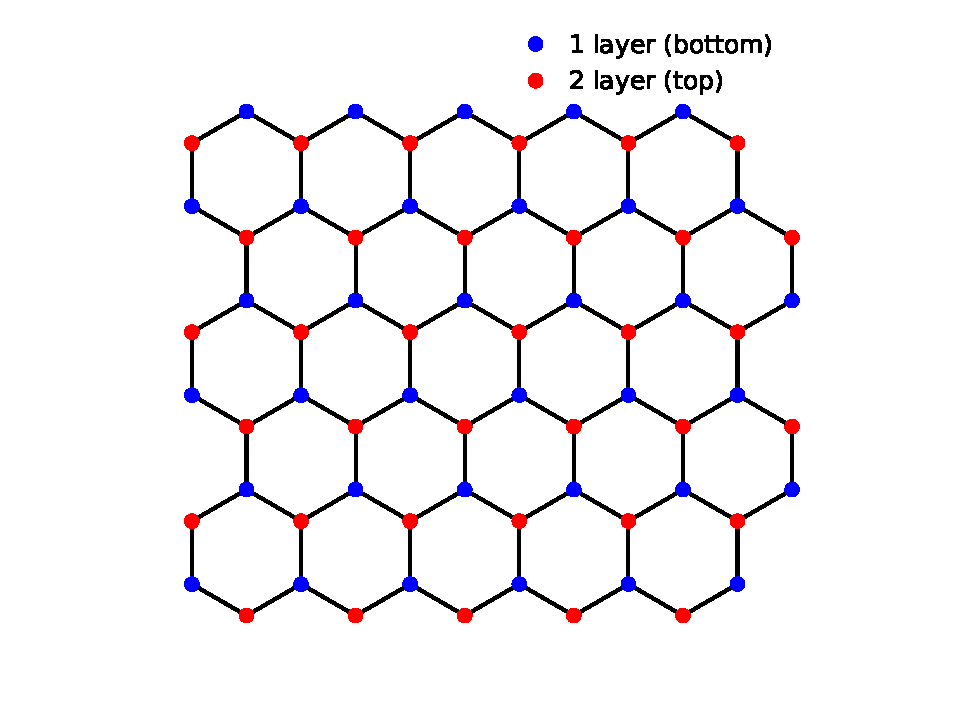
\includegraphics[width=0.48\textwidth]{pic/moire_lattice.pdf}
    }
    \subfigure[moiré BZ and BZ]{
        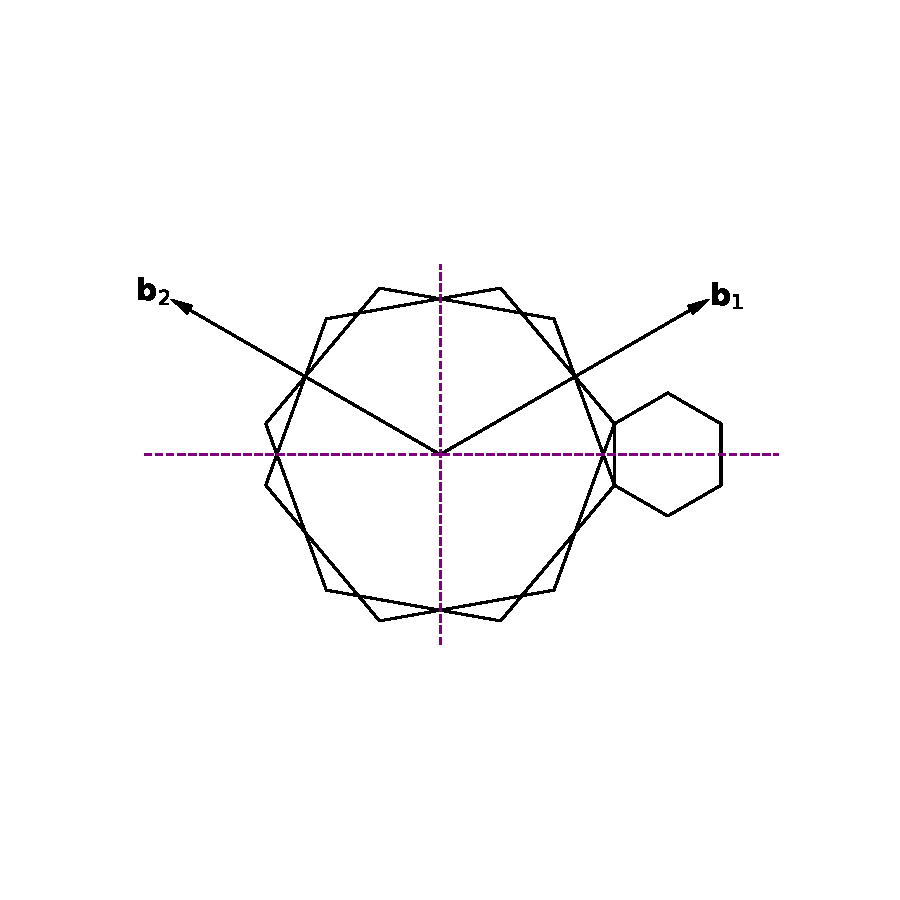
\includegraphics[width=0.48\textwidth]{pic/mBZ_BZ.pdf}
    }
    \caption{Geometry}
    % \label{fig1}
\end{figure}

\begin{itemize}
	\item Commensurate Structure
\end{itemize}

\section{Bistritzer-Macdonald Model}

\subsection{Diagonal Term: Intra-Layer Coupling}
We can write the diagonal term like the energyband folding 
\begin{align}
	H = \sum_{\bm{k}} \begin{pmatrix}
		\hat{c}^{\dagger}_{\bm{k},\bm{K}^{t}} & \hat{c}^{\dagger}_{\bm{k},\bm{K}^{b}} & \hat{c}^{\dagger}_{\bm{k} + \bm{b}^{m}_{2}, \bm{K}^{t}} & \hat{c}^{\dagger}_{\bm{k} + \bm{b}^{m}_{2},\bm{K}^{b}} & \cdots
	\end{pmatrix}
	H_{intra}\p{\bm{k}}
	\begin{pmatrix}
		\hat{c}_{\bm{k},\bm{K}^{t}} \\ \hat{c}_{\bm{k},\bm{K}^{b}} \\ \hat{c}_{\bm{k} + \bm{b}^{m}_{2}, \bm{K}^{t}} \\ \hat{c}_{\bm{k} + \bm{b}^{m}_{2},\bm{K}^{b}} \\ \cdots
	\end{pmatrix},
\end{align}
where \(\hat{c}_{\bm{k},\bm{K}^{t}}\) contains two sublattice \(\br{A, B}\), which is 
\begin{align}
	\hat{c}_{\bm{k},\bm{K}^{i}} = \begin{pmatrix}
		\hat{a}_{\bm{k},\bm{K}^{i}} & \hat{b}_{\bm{k},\bm{K}^{i}}
	\end{pmatrix}  \quad i \in {t, b}.
\end{align}
Thus the corresponding state is 
\begin{align}
	\ket{\bm{k} + n_1 \bm{b}^{m}_{1} + n_2 \bm{b}^{m}_{2},\, \bm{K}^{t/b}, \, A/B},
\end{align}
where the \(\bm{k} + n_1 \bm{b}^{m}_{1} + n_2 \bm{b}^{m}_{2}\) is the wave vector we choose in the k-space with \(\bm{K}^{t}\) as the origin. \(\bm{K}^{t/b}\) is equivalent to the layer index where valley index is hidden within \(\bm{K}^{t/b}\) and \(A/B\) is the sublattice index. In the following, we will omit the sublattice index. The Bloch matrix is 
\begin{align}
	H_{intra}\p{\bm{k}} = v_{F}	\begin{pmatrix}
		\p{\bm{k} - \bm{K}^{t}} \cdot\hat{\sigma}^{\te/2} & 0 & 0 & 0 & \cdots \\
		0 &  \p{\bm{k} - \bm{K}^{b}} \cdot \hat{\sigma}^{- \te/2}& 0 & 0 &  \cdots \\
		0 & 0 & \p{\bm{k} + \bm{b}^{m}_{2} - \bm{K}^{t}} \cdot \hat{\sigma}^{\te/2} & 0 &  \cdots \\
		0 & 0 & 0 & \p{\bm{k} + \bm{b}^{m}_{2} - \bm{K}^{b}} \cdot \hat{\sigma}^{- \te/2} & \cdots \\
		\vdots
	\end{pmatrix} .
\end{align}

Now we add the reciprocal lattice basis vectors to the \(\bm{K}^{t}\) and \(\bm{K}^{b}\), which is equivalent to \(\bm{k} \) minus the reciprocal lattice basis vectors. So the state is 
\begin{align}
	\ket{\bm{k} + n_{1} \bm{b}^{m}_{1} + n_{2} \bm{b}^{m}_{2}, \bm{K}^{t/b}} = \ket{\bm{k}, \bm{K}^{t/b} - n_{1} \bm{b}^{m}_{1} - n_{2} \bm{b}^{m}_{2}}.
\end{align}
Thus the Hamiltonian is
\begin{align}
	\hat{H} = \sum_{\bm{k}} \begin{pmatrix}
		\hat{c}^{\dagger}_{\bm{k},\bm{K}^{t}} & \hat{c}^{\dagger}_{\bm{k},\bm{K}^{b}} & \hat{c}^{\dagger}_{\bm{k} , \bm{K}^{t} - \bm{b}^{m}_{2}} & \hat{c}^{\dagger}_{\bm{k},\bm{K}^{b} - \bm{b}^{m}_{2}} & \cdots
	\end{pmatrix}
	H_{intra}\p{\bm{k}}
	\begin{pmatrix}
		\hat{c}_{\bm{k},\bm{K}^{t}} \\ \hat{c}_{\bm{k},\bm{K}^{b}} \\ \hat{c}_{\bm{k}, \bm{K}^{t} - \bm{b}^{m}_{2}} \\ \hat{c}_{\bm{k} ,\bm{K}^{b} - \bm{b}^{m}_{2}} \\ \cdots
	\end{pmatrix},
\end{align}
and the Bloch matrix is
\begin{align}
	H_{intra}\p{\bm{k}} = v_{F}	\begin{pmatrix}
		\p{\bm{k} - \bm{K}^{t}} \cdot\hat{\sigma}^{\te/2} & 0 & 0 & 0 & \cdots \\
		0 &  \p{\bm{k} - \bm{K}^{b}} \cdot \hat{\sigma}^{- \te/2}& 0 & 0 &  \cdots \\
		0 & 0 & \p{\bm{k}  -\p{ \bm{K}^{t} - \bm{b}^{m}_{2}}} \cdot \hat{\sigma}^{\te/2} & 0 &  \cdots \\
		0 & 0 & 0 & \p{\bm{k}  - \p{\bm{K}^{b} - \bm{b}^{m}_{2}}} \cdot \hat{\sigma}^{- \te/2} & \cdots \\
		\vdots
	\end{pmatrix} .
\end{align}
The matrix term is 
\begin{align}
	\begin{split}
		\braket{\bm{k}, \bm{K}^{b} + n_{1} \bm{b}^{m}_{1} + n_{2} \bm{b}^{m}_{2}| \hat{H} |\bm{k}, \bm{K}^{b} + n_{1} \bm{b}^{m}_{1} + n_{2} \bm{b}^{m}_{2} } &= \bb{\bm{k} - \p{\bm{K}^{b} + n_{1} \bm{b}^{m}_{1} + n_{2} \bm{b}^{m}_{2}}}\cdot \hat{\sigma}^{- \te/2}  \\
		\braket{\bm{k}, \bm{K}^{t} + m_{1} \bm{b}^{m}_{1} + m_{2} \bm{b}^{m}_{2}| \hat{H}|\bm{k}, \bm{K}^{t} + m_{1} \bm{b}^{m}_{1} + m_{2} \bm{b}^{m}_{2} } &= \bb{\bm{k} - \p{\bm{K}^{t} + m_{1} \bm{b}^{m}_{1} + m_{2} \bm{b}^{m}_{2}}}\cdot \hat{\sigma}^{\te/2}.
	\end{split}
\end{align}


\subsection{Off-Diagonal Term: Inter-Layer Tunneling}
Considering a state with momentum \(\bm{k}^{t}\) on the top layer \(\beta\) sublattice hopping to the state with momentum \(\bm{k}^b\) on the bottom layer \(\beta\) sublattice, which is  
\begin{align}
	T^{\alpha,\beta}_{\bm{k}^{b},\bm{k}^{t}} = \braket{\psi^{b}_{\bm{k}^{b},\alpha} | H_{inter} | \psi^{t}_{\bm{k}^{t},\beta}}.
\end{align}

The Bloch wave functions are 
\begin{align}
	\ket{\psi^{b}_{\bm{k}^{b},\alpha}}  &= \frac{1}{\sqrt{N_1 N_2}} \sum_{\bm{R}^{b}_{n_1 n_2}} e^{i \bm{k}^{b} \cdot \bm{R}^{b}_{n_1 n_2}} \ket{\bm{R}^{b}_{n_1 n_2} + \bm{\tau}^{b}_{\alpha}} \\
	\ket{\psi^{t}_{\bm{k}^{t} ,\beta}} &= \frac{1}{\sqrt{N_1 N_2}} \sum_{\bm{R}^{t}_{m_1 m_2}} e^{i \bm{k}^{t} \cdot \bm{R}^{t}_{m_1 m_2}} \ket{\bm{R}^{t}_{m_1 m_2} + \bm{\tau}^{t}_{\beta}}.
\end{align}
which leads to 
\begin{align}
	T^{\alpha,\beta}_{\bm{k}^{b},\bm{k}^{t}} = \frac{1}{N_1 N_2} \sum_{\bm{R}^{b}_{n_1 n_2}} \sum_{\bm{R}^{t}_{m_1 m_2}}  e^{- i \bm{k}^{b} \cdot \bm{R}^{b}_{n_1 n_2}} e^{i \bm{k}^{t} \cdot  \bm{R}^{t}_{m_1 m_2}} \braket{\bm{R}^{b}_{n_1 n_2} + \bm{\tau}^{b}_{\alpha}| H_{inter} | \bm{R}^{t}_{m_1 m_2} + \bm{\tau}^{t}_{\beta}},
\end{align} 
 
The interlayer coupling in real space satisfies the translation symmetry, so we rewrite it with Fourier transform
\begin{align}
	\begin{split}
		\braket{\bm{R}^{b}_{n_1 n_2} + \bm{\tau}^{b}_{\alpha}| H_{inter} | \bm{R}^{t}_{m_1 m_2} + \bm{\tau}^{t}_{\beta}} & = t_{\perp} \p{\bm{R}^{b}_{n_1 n_2} + \bm{\tau}^{b}_{\alpha} - \bm{R}^{t}_{m_1 m_2}  - \bm{\tau}^{t}_{\beta}} \\
		& = \int \frac{d^{2} \bm{k}}{\p{2 \pi}^2} t_{\perp}\p{\bm{k}} e^{  i \bm{k} \cdot \p{\bm{R}^{b}_{n_1 n_2} + \bm{\tau}^{b}_{\alpha} - \bm{R}^{t}_{m_1 m_2}  - \bm{\tau}^{t}_{\beta}} }\\
		& =\frac{1}{N_1 N_2} \sum_{\bm{k} \in \Delta q^2 \mathbb{Z}^2} \frac{t_{\perp} \p{\bm{k}}}{A_{u.c.}} e^{  i \bm{k} \cdot \p{\bm{R}^{b}_{n_1 n_2} + \bm{\tau}^{b}_{\alpha} - \bm{R}^{t}_{m_1 m_2}  - \bm{\tau}^{t}_{\beta}} },
	\end{split}
\end{align}
where the integral can be changed into a sum
\begin{align}
	\int d^{2} \bm{k} = \sum_{\bm{k} \in {\p{\frac{2 \pi n_{1}}{N_{1} \bm{a}_{1}}, \frac{2 \pi n_{2}}{N_{2} \bm{a}_{2}}}}} \Delta q_{1} \Delta q_{2} =\sum_{\bm{k} \in \Delta q^2 \mathbb{Z}^2}  \frac{2 \pi}{N_{1} \bm{a}_{1}} \frac{2 \pi}{N_{2} \bm{a}_{2}}=\frac{\p{2 \pi}^2}{N_1 N_2 A_{u.c.} } \sum_{\bm{k} \in \Delta q^2 \mathbb{Z}^2},  
\end{align}
and \(A_{u.c.} = \bm{a}_{1} \cdot \bm{a}_{2}\) is the area of the unit. 

The hopping term is 
\begin{align}
	\begin{split}
		\braket{\psi^{b}_{\bm{k}^{b},\alpha} | H_{inter} | \psi^{t}_{\bm{k}^{t},\beta}} &=
		\frac{1}{\p{N_1 N_2}^2} \sum_{\bm{R}^{b}_{n_1 n_2}} \sum_{\bm{R}^{t}_{m_1 m_2}} \sum_{\bm{k}} \frac{t_{\perp} \p{\bm{k}}}{A_{u.c.}} e^{- i \bm{k}^{b} \cdot \bm{R}^{b}_{n_1 n_2}} e^{i \bm{k}^{t} \cdot  \bm{R}^{t}_{m_1 m_2}} e^{  i \bm{k} \cdot \p{\bm{R}^{b}_{n_1 n_2} + \bm{\tau}^{b}_{\alpha} - \bm{R}^{t}_{m_1 m_2}  - \bm{\tau}^{t}_{\beta}} },
	\end{split}
\end{align}
where the form of the delta function should correspond to the field operators \(\psi\) and \(\psi^\dagger\). We expand \(\bm{k}^{b}\) and \(\bm{k}^{t}\) around \(\bm{K}^{b}\) and \(\bm{K}^{t}\)
\begin{align}
	\bm{k}^{b} = \bm{K}^{b} + \bm{p}^{b}, \quad \bm{k}^{t} = \bm{K}^{t} + \bm{p}^{t},
\end{align}
where \(\bm{p}^{b}\) and \(\bm{p}^{t}\) are the infinitesimal quantity, which lead to 
\begin{align}
	\begin{split}
		T^{\alpha, \beta}_{\bm{k}^{b}, \bm{k}^{t}} & = \frac{1}{\p{N_1 N_2}^2} \sum_{\bm{R}^{b}_{n_1 n_2}} \sum_{\bm{R}^{t}_{m_1 m_2}} \sum_{\bm{k}} \frac{t_{\perp} \p{\bm{k}}}{A_{u.c.}} e^{- i \p{\bm{K}^{b} + \bm{p}^{b}} \cdot \bm{R}^{b}_{n_1 n_2}} e^{i\p{\bm{K}^{t} + \bm{p}^{t}} \cdot  \bm{R}^{t}_{m_1 m_2}} e^{  i \bm{k} \cdot \p{\bm{R}^{b}_{n_1 n_2} + \bm{\tau}^{b}_{\alpha} - \bm{R}^{t}_{m_1 m_2}  - \bm{\tau}^{t}_{\beta}} } \\
		& = \frac{1}{\p{N_1 N_2}^2} \sum_{\bm{R}^{b}_{n_1 n_2}} \sum_{\bm{R}^{t}_{m_1 m_2}} \sum_{\bm{k}} \frac{t_{\perp} \p{\bm{k}}}{A_{u.c.}} e^{ i \bb{\bm{k} - \p{\bm{K}^{b} + \bm{p}^{b}}} \cdot \bm{R}^{b}_{n_1 n_2}}  e^{  - i \bb{\bm{k} - \p{\bm{K}^{t} + \bm{p}^{t}}} \cdot \bm{R}^{t}_{m_1 m_2}} e^{i \bm{k} \cdot \bm{\tau}^{b}_{\alpha} } e^{ - i \bm{k} \cdot \bm{\tau}^{t}_{\beta} }.
	\end{split}
\end{align}

We use the orthogonality relations
\begin{align}
	\sum_{\bm{R}^{b}_{n_1 n_2}}e^{ i \bb{\bm{k} - \p{\bm{K}^{b} + \bm{p}^{b}}} \cdot \bm{R}^{b}_{n_1 n_2}} &= 
	\begin{cases} 
	N_1 N_2 & \text{if } \bm{k} - \p{\bm{K}^{b} + \bm{p}^{b}} = \bm{G}^{b}_{\mu \nu} ,\, \mu, \nu \in \mathbb{Z}\\
	0 & \text{otherwise} 
	\end{cases} \\
	\sum_{\bm{R}^{t}_{m_1 m_2}} e^{  - i \bb{\bm{k} - \p{\bm{K}^{t} + \bm{p}^{t}}} \cdot \bm{R}^{t}_{m_1 m_2}} &=
	 \begin{cases}
		N_1 N_2  & \text{if } \bm{k} - \p{\bm{K}^{t} + \bm{p}^{t}} = \bm{G}^{t}_{\rho \sigma}, \, \rho,\sigma \in \mathbb{Z}\\
		0 & \text{otherwise} 
	\end{cases},
\end{align}
which is 
\begin{align}
	\bm{R}^{b}_{n_1 n_2} \cdot \bm{G}^{b}_{\mu \nu} =  \bm{R}^{t}_{m_1 m_2} \cdot  \bm{G}^{t}_{\rho \sigma} = 2 \pi,
\end{align}
Also the $\bm{k}$ must satisfies 
\begin{align}
	\bm{k} = \bm{K}^b + \bm{p}^b + \bm{G}^{b}_{\mu \nu} = \bm{K}^{t} + \bm{p}^{t}+ \bm{G}^{t}_{\rho \sigma}.
\end{align}

With AA-stacking we get 
\begin{align}
	\begin{split}
		T^{\alpha, \beta}_{\bm{k}^{b}, \bm{k}^{t}} &= \sum_{\bm{k}} \frac{t_{\perp} \p{\bm{k}}}{A_{u.c.}} e^{i \bm{k} \cdot \bm{\tau}^{b}_{\alpha}}  e^{-i \bm{k} \cdot \bm{\tau}^{t}_{\beta}} \delta_{\bm{K}^b + \bm{p}^b + \bm{G}^{b}_{\mu \nu},  \bm{K}^{t} + \bm{p}^{t}+ \bm{G}^{t}_{\rho \sigma}}\\
		& = \sum_{\bm{k}} \frac{t_{\perp} \p{\bm{k}}}{A_{u.c.}} e^{i \p{\bm{K}^b + \bm{p}^b + \bm{G}^{b}_{\mu \nu}} \cdot \bm{\tau}^{b}_{\alpha}}  e^{-i \p{\bm{K}^{t} + \bm{p}^{t}+ \bm{G}^{t}_{\rho \sigma}} \cdot \bm{\tau}^{t}_{\beta}} \delta_{\bm{K}^b + \bm{p}^b + \bm{G}^{b}_{\mu \nu},  \bm{K}^{t} + \bm{p}^{t}+ \bm{G}^{t}_{\rho \sigma}} \\
		& = \sum_{\bm{k}} \frac{t_{\perp} \p{\bm{k}}}{A_{u.c.}} e^{i \p{\bm{K}^b + \bm{p}^b} \cdot \bm{\tau}^{b}_{\alpha}} e^{-i \p{\bm{K}^{t} + \bm{p}^{t}} \cdot \bm{\tau}^{t}_{\beta}} e^{i \bm{G}^{b}_{\mu \nu} \cdot \bm{\tau}^{b}_{\alpha}} e^{-i \bm{G}^{t}_{\rho \sigma} \cdot \bm{\tau}^{t}_{\beta}} \delta_{\bm{K}^b + \bm{p}^b + \bm{G}^{b}_{\mu \nu},  \bm{K}^{t} + \bm{p}^{t}+ \bm{G}^{t}_{\rho \sigma}}. \\
	\end{split}
\end{align}
Since \(|\bm{p}^{b}| \ll |\bm{K}^{b}|\) and \(|\bm{p}^{t}| \ll |\bm{K}^{t}|\), we rewrite it as 
\begin{align}
	\begin{split}
		T^{\alpha, \beta}_{\bm{k}^{b}, \bm{k}^{t}} &= \sum_{\bm{k}} \frac{t_{\perp} \p{\bm{k}}}{A_{u.c.}} e^{i \bm{K}^b \cdot \bm{\tau}^{b}_{\alpha}} e^{-i \bm{K}^{t} \cdot \bm{\tau}^{t}_{\beta}} e^{i \bm{G}^{b}_{\mu \nu} \cdot \bm{\tau}^{b}_{\alpha}} e^{-i \bm{G}^{t}_{\rho \sigma} \cdot \bm{\tau}^{t}_{\beta}} \delta_{\bm{K}^b + \bm{p}^b + \bm{G}^{b}_{\mu \nu},  \bm{K}^{t} + \bm{p}^{t}+ \bm{G}^{t}_{\rho \sigma}} \\
		& = \sum_{\bm{k}} \frac{t_{\perp} \p{\bm{k}}}{A_{u.c.}} e^{i \bm{K} \cdot \bm{\tau}_{\alpha}} e^{-i \bm{K} \cdot \bm{\tau}_{\beta}} e^{i \bm{G}_{\mu \nu} \cdot \bm{\tau}_{\alpha}} e^{-i \bm{G}_{\rho \sigma} \cdot \bm{\tau}_{\beta}} \delta_{\bm{K}^b + \bm{p}^b + \bm{G}^{b}_{\mu \nu},  \bm{K}^{t} + \bm{p}^{t}+ \bm{G}^{t}_{\rho \sigma}} \\
		& = \sum_{\bm{k}} \frac{t_{\perp} \p{\bm{k}}}{A_{u.c.}} e^{i \bm{K} \cdot \p{\bm{\tau}_{\alpha} - \bm{\tau}_{\beta}}}  e^{i \p{\bm{G}_{\mu \nu} \cdot \bm{\tau}_{\alpha} - \bm{G}_{\rho \sigma} \cdot \bm{\tau}_{\beta}}} \delta_{\bm{K}^b + \bm{p}^b + \bm{G}^{b}_{\mu \nu},  \bm{K}^{t} + \bm{p}^{t}+ \bm{G}^{t}_{\rho \sigma}},
	\end{split}
\end{align}
and we change the summation index
\begin{align}
	\begin{split}
		T^{\alpha, \beta}_{\bm{K}^{b} + \bm{p}^{b} + \bm{G}^{b}_{\mu \nu}, \bm{K}^{t} + \bm{p}^{t}+ \bm{G}^{t}_{\rho \sigma}}  & = \sum_{\bm{G}^{b}_{\mu \nu}} \sum_{\bm{G}^{t}_{\rho \sigma}} \frac{t_{\perp} \p{\bm{K}^b  + \bm{G}^{b}_{\mu \nu}}}{A_{u.c.}}  e^{i \bm{K} \cdot \p{\bm{\tau}_{\alpha} - \bm{\tau}_{\beta}}} e^{i \p{\bm{G}^{b}_{\mu \nu} \cdot \bm{\tau}^{b}_{\alpha} - \bm{G}^{t}_{\rho \sigma} \cdot \bm{\tau}^{t}_{\beta}}} \delta_{\bm{K}^b + \bm{p}^b + \bm{G}^{b}_{\mu \nu},  \bm{K}^{t} + \bm{p}^{t}+ \bm{G}^{t}_{\rho \sigma}} \\
		&= \sum_{\bm{G}^{b}_{\mu \nu}} \sum_{\bm{G}^{t}_{\rho \sigma}} \frac{t_{\perp} \p{\bm{K}^b  + \bm{G}^{b}_{\mu \nu}}}{A_{u.c.}} e^{i \p{\bm{G}^{b}_{\mu \nu} \cdot \bm{\tau}^{b}_{\alpha} - \bm{G}^{t}_{\rho \sigma} \cdot \bm{\tau}^{t}_{\beta}}} \delta_{\bm{K}^b + \bm{p}^b + \bm{G}^{b}_{\mu \nu},  \bm{K}^{t} + \bm{p}^{t}+ \bm{G}^{t}_{\rho \sigma}},
	\end{split}
\end{align}
where \(\bm{K} \cdot \p{\bm{\tau}_{\alpha} - \bm{\tau}_{\beta}} = 0\).

\begin{figure}[h!]  % h:与源文本位于同一位置 !:覆盖
	\begin{center}
		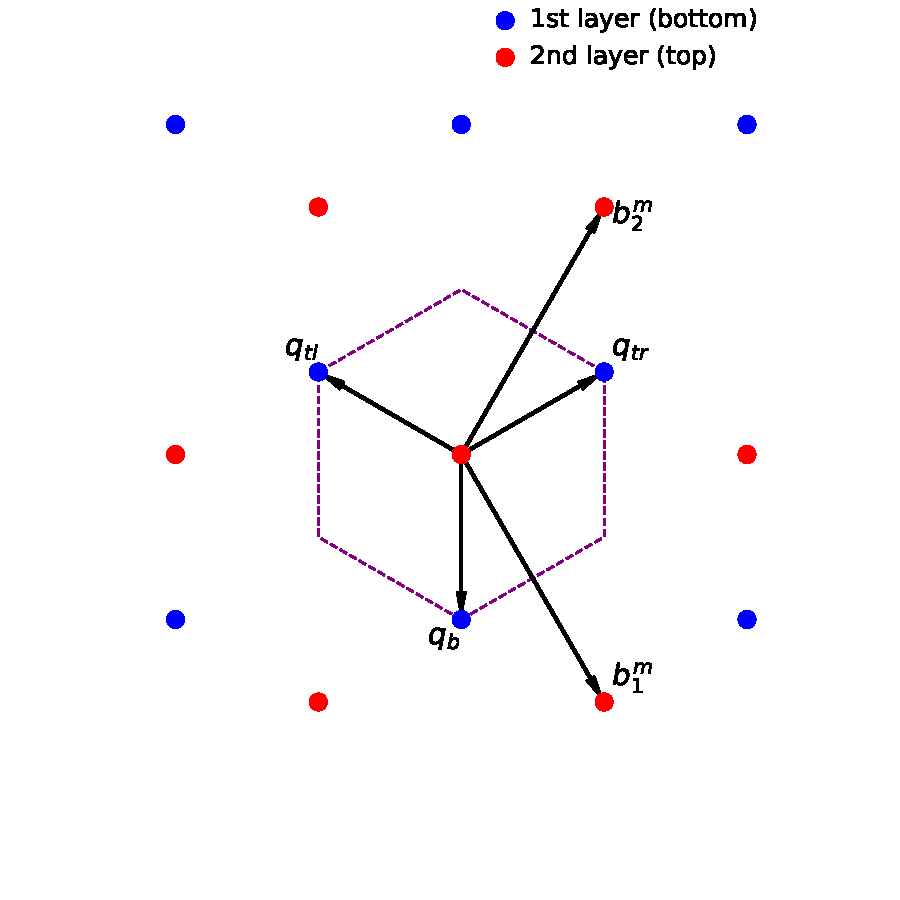
\includegraphics[width=0.5\textwidth]{pic/K_lattice.pdf}
	\end{center}
	\caption{Hopping Processes}
\end{figure}

\begin{itemize}
	\item \(\mb{K}_M\)-centered Tripod Model
\end{itemize}

Since \(t_{\perp} \p{\bm{k}}\) decays rapidly as a function of \(|\bm{k}|\), the main contribution to the sum comes from the nearest same valley \(\bm{G} \in \br{0, \bm{b}_{2}, -\bm{b}_1} \) which is 
\begin{align}
	|\bm{K}^b  + \bm{G}^{b}_{\mu \nu}| = |\bm{K}^{b}|  \Leftrightarrow \bm{G}^{b}_{\mu \nu} \in \br{0, \bm{b}^{b}_{2}, -\bm{b}^{b}_1},
\end{align}


The tunneling between two nearest different valley is hard to occur because of the change of momentum is huge. So the interlayer hopping between same valley is 
\begin{align}
    \begin{split}
        T^{\alpha, \beta}_{\bm{K}^{b} + \bm{p}^{b} + \bm{G}^{b}_{\mu \nu}, \bm{K}^{t} + \bm{p}^{t} + \bm{G}^{t}_{\rho \sigma}} \approx \frac{t_{\perp} \p{|\bm{K}|}}{A_{u.c.}} \sum_{\bm{G}^{t}_{\rho \sigma}\p{\bm{G}_{\rho \sigma}}} & \left\{  e^{-i  \bm{G}_{\rho \sigma} \cdot \bm{\tau}_{\beta} }  \delta_{\bm{K}^b + \bm{p}^b,  \bm{K}^{t} + \bm{p}^{t} + \bm{G}^{t}_{\rho \sigma}} + e^{i \p{\bm{b}_{2} \cdot \bm{\tau}_{\alpha} - \bm{G}_{\rho \sigma} \cdot  \bm{\tau}_{\beta}} } \delta_{\bm{K}^b + \bm{p}^b + \bm{b}^{b}_{2},  \bm{K}^{t} + \bm{p}^{t}+ \bm{G}^{t}_{\rho \sigma}} \right. \\
        & \quad \left. + e^{-i \p{\bm{b}_{1} \cdot \bm{\tau}_{\alpha} + \bm{G}_{\rho \sigma} \cdot \bm{\tau}_{\beta}}} \delta_{\bm{K}^b + \bm{p}^b - \bm{b}^{b}_{1},  \bm{K}^{t} + \bm{p}^{t}+ \bm{G}^{t}_{\rho \sigma}} \right\}.
    \end{split}
\end{align}
 To satisfy the condition of Kronecker delta function when \(\te \rightarrow 0\), \( \bm{G}_{\rho \sigma}^{t} \) must also only be \( \br{0, -\bm{b}_{1}^{t}, \bm{b}_{2}^{t} }\) or  \(\bm{G}_{\rho \sigma} \in \br{ 0, -\bm{b}_{1}, \bm{b}_{2}}\). The hopping term changes into 
\begin{align}
	\begin{split}
		T^{\alpha, \beta}_{\bm{K}^{b} + \bm{p}^{b} + \bm{G}^{b}_{\mu \nu}, \bm{K}^{t} + \bm{p}^{t} + \bm{G}^{t}_{\rho \sigma}} =  \frac{t_{\perp} \p{|\bm{K}|}}{A_{u.c.}}  \left\{  \delta_{\bm{K}^b + \bm{p}^b,  \bm{K}^{t} + \bm{p}^{t}} + e^{i \bm{b}_{2} \cdot \p{\bm{\tau}_{\alpha} - \bm{\tau}_{\beta}}} \delta_{\bm{K}^{b} + \bm{p}^{b}_{1} + \bm{b}^{b}_{2},  \bm{K}^{t} + \bm{p}^{t}_{2}+ \bm{b}^{t}_{2}}  
		+ e^{-i \bm{b}_{1} \cdot \p{\bm{\tau}_{\alpha} - \bm{\tau}_{\beta}} } \delta_{\bm{K}^{b} + \bm{p}^{b}_1 - \bm{b}^{b}_{1},  \bm{K}^{t} + \bm{p}^{t}_{2}- \bm{b}^{t}_{1}}\right\}.
	\end{split}
\end{align}

We rewrite the hopping term in matrix form and omit the sublattice index 
\begin{align}
	T_{\bm{K}^{b} + \bm{p}^{b}+ \bm{G}^{b}_{\mu \nu}, \bm{K}^{t} + \bm{p}^{t} + \bm{G}^{t}_{\rho \sigma}} = \begin{bmatrix}
		T^{A A} & T^{A B} \\
		T^{B A} & T^{B B}
	\end{bmatrix}
\end{align}
which is
\begin{align}
	\begin{split}
		T_{\bm{K}^{b} + \bm{p}^{b}+ \bm{G}^{b}_{\mu \nu}, \bm{K}^{t} + \bm{p}^{t} + \bm{G}^{t}_{\rho \sigma}} = & \frac{t_{\perp} \p{|\bm{K}|}}{A_{u.c.}} \bb{T_{\bm{q}_{b}} \delta_{\bm{p}^{t} - \bm{p}^{b}, \bm{K}^{b} - \bm{K}^{t}} + T_{\bm{q}_{tr}} \delta_{\bm{p}^{t} - \bm{p}^{b}, \p{\bm{K}^{b} + \bm{b}^{b}_{2}} - \p{\bm{K}^{t} + \bm{b}^{t}_{2}}} + T_{\bm{q}_{tl}} \delta_{\bm{p}^{t} - \bm{p}^{b}, \p{\bm{K}^{b} - \bm{b}^{b}_{1}} - \p{\bm{K}^{t} - \bm{b}^{t}_{1}}}}  \\
		& = T_{\bm{q}_{b}} \delta_{\bm{p}^{t} - \bm{p}^{b}, \bm{q}_{b}} + T_{\bm{q}_{tr}} \delta_{\bm{p}^{t}- \bm{p}^{b}, \bm{q}_{tr}} + T_{\bm{q}_{tl}} \delta_{\bm{p}^{t} - \bm{p}^{b}, \bm{q}_{tl}}.
	\end{split}
\end{align}
where the tunneling vectors are
\begin{align}
	\bm{q}_{b}=\bm{K}^{b}-\bm{K}^{t},\quad 
	\bm{q}_{tr}=\p{\bm{K}^{b} + \bm{b}^{b}_{2}} - \p{\bm{K}^{t} + \bm{b}^{t}_{2}} = \bm{q}_{b} + \bm{b}^{m}_{2} , \quad 
	\bm{q}_{tl} = \p{\bm{K}^{b} - \bm{b}^{b}_{1}} - \p{\bm{K}^{t} - \bm{b}^{t}_{1}} = \bm{q}_{b} - \bm{b}^{m}_{1},
\end{align}
\begin{align}
	\bm{q}_{1}=\frac{8\pi\sin(\theta/2)}{3a}(0,-1),\quad 
	\bm{q}_{2}=\frac{8\pi\sin(\theta/2)}{3a}(\sqrt{3}/2,1/2),\quad
	\bm{q}_{3}=\frac{8\pi\sin(\theta/2)}{3 a}(-\sqrt{3}/2,1/2),
\end{align}
and the matrices \(T_{\bm{q}_{b}}, \,  T_{\bm{q}_{tr}} , \, T_{\bm{q}_{tl}}\) are
\begin{align}
	T_{\bm{q}_{b}} = \begin{bmatrix}1&1\\1&1\end{bmatrix}, \quad
	T_{\bm{q}_{tr}} = \begin{bmatrix} 1 & e^{-i \frac{2 \pi}{3}} \\ 
		e^{i \frac{2 \pi}{3}} & 1 
	\end{bmatrix}, \quad 
	T_{\bm{q}_{tl}} = \begin{bmatrix} 1 & e^{i \frac{2 \pi}{3}} \\
		e^{-i \frac{2 \pi}{3}} & 1\end{bmatrix}.
\end{align}
More generally
\begin{align} \label{eq91}
	\braket{\bm{k}, \bm{K}^{b} + n_{1} \bm{b}^{m}_{1} + n_{2} \bm{b}^{m}_{2}| \hat{H}|\bm{k}, \bm{K}^{t} + m_{1} \bm{b}^{m}_{1} + m_{2} \bm{b}^{m}_{2} } = \begin{cases}
		&T_{\bm{q}_{b}} ,\quad n_1 = m_1,\, n_2 = m_2 \\
		&T_{\bm{q}_{tr}}, \quad n_1 = m_1,\, n_2 = m_2 +1 \\
		&T_{\bm{q}_{tl}}, \quad n_1 = m_1-1,\, n_2 = m_2
	\end{cases}
\end{align}

\subsection{Constructing Hamiltonian}
We discuss the delta function in detail. For \(\bm{G}_{\mu \nu}^{b} = \bm{G}_{\rho \sigma}^{t} = 0\) and  \(\bm{p}^{t} - \bm{p}^{b} = \bm{q}_{b}\) 
\begin{align}
	\braket{\bm{K}^{b} + \bm{p}^{b}|H_{inter} \p{\bm{k}}|\bm{K}^{t} + \bm{p}^{t}} = \braket{\bm{K}^{b} + \bm{p}^{t} -\bm{q}_{b} |H_{inter} \p{\bm{k}}|\bm{K}^{t} + \bm{p}^{t}} = \frac{t_{\perp} \p{|\bm{K}|}}{A_{u.c.}} T_{\bm{q}_{b}}.
\end{align}
We rewrite the ket
\begin{align}
	\ket{\bm{K}^{b} + \bm{p}^{t} -\bm{q}_{b}} \Rightarrow \ket{\bm{k},\bm{K}^{b}} ,\quad \ket{\bm{K}^{t} + \bm{p}^{t}} \Rightarrow \ket{\bm{k}, \bm{K}^{t}}.
\end{align}
where \(\bm{p}^{t} = \bm{k}\) if we set the \(\bm{K}^{t}\) as the new origin. So the off-diagonal term is 
\begin{align}
	\braket{\bm{k},\bm{K}^{b} |H_{inter} \p{\bm{k}} |\bm{k}, \bm{K}^{t} } =  \frac{t_{\perp} \p{|\bm{K}|}}{A_{u.c.}} T_{\bm{q}_{b}},
\end{align}
and the corresponding diagonal term is 
\begin{align}
	\braket{\bm{k},\bm{K}^{b} |H_{intra} \p{\bm{k}} |\bm{k}, \bm{K}^{b} } = \bm{p}^{b} \cdot \hat{\sigma}^{-\te/2} = \p{\bm{k} - \bm{K}^{b}}\cdot \hat{\sigma}^{-\te/2}
\end{align}

\begin{figure}[h!]
    \centering
    \subfigure[Process I]{
        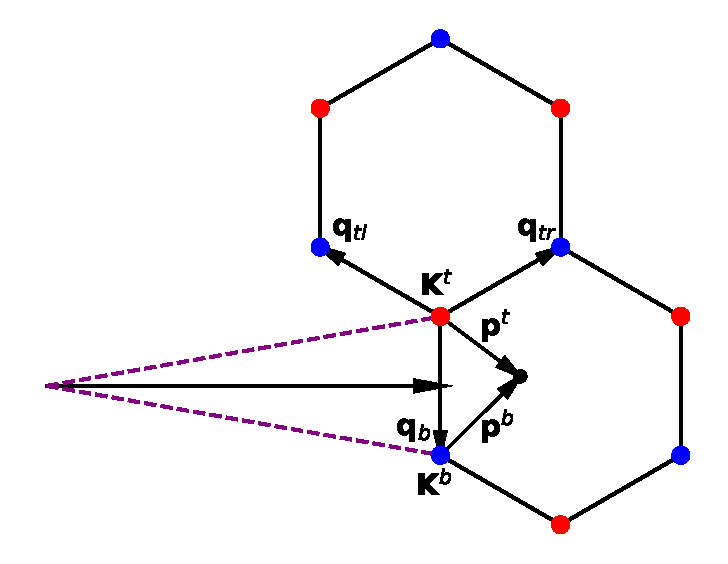
\includegraphics[width=0.45\textwidth]{pic/qb.pdf}
    }
    \subfigure[Process II]{
        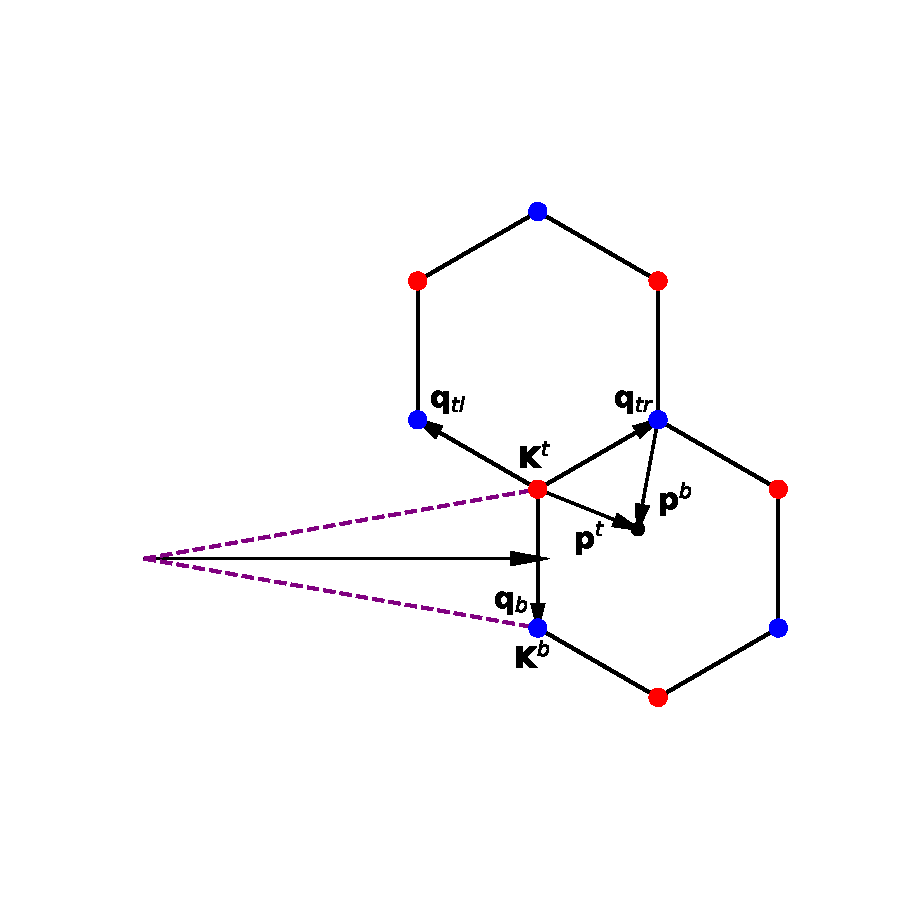
\includegraphics[width=0.45\textwidth]{pic/qtr.pdf}
    }
    \caption{Intra-Tunneling Process}
    \label{fig:two_side_by_side}
\end{figure}
For  \(\bm{G}_{\mu \nu}^{b} = \bm{b}^{b}_{2},\, \bm{G}_{\rho \sigma}^{t} = \bm{b}^{t}_{2}\) and \(\bm{p}^{t} - \bm{p}^{b} = \bm{q}_{tr}\)
\begin{align}
	\begin{split}
		&\braket{\bm{K}^{b} + \bm{p}^{b} + \bm{b}^{b}_{2} |H_{inter} \p{\bm{k}}|\bm{K}^{t} + \bm{p}^{t} + \bm{b}^{t}_{2} } = \braket{\bm{K}^{b} + \bm{p}^{t} -\bm{q}_{tr} + \bm{b}^{b}_{2} |H_{inter} \p{\bm{k}}|\bm{K}^{t} + \bm{p}^{t} + \bm{b}^{t}_{2} } \\
		 = &\braket{\bm{K}^{b} + \bm{p}^{t} -\bm{q}_{tr} + \bm{b}^{b}_{2} - \bm{b}^{t}_{2} |H_{inter} \p{\bm{k}}|\bm{K}^{t} + \bm{p}^{t}  } = \braket{\bm{K}^{b} + \bm{p}^{t} -\bm{q}_{tr} + \bm{b}^{m}_{2} |H_{inter} \p{\bm{k}}|\bm{K}^{t} + \bm{p}^{t}  }.
	\end{split}
\end{align}
We defined
\begin{align}
	\ket{\bm{K}^{b} + \bm{p}^{t} -\bm{q}_{tr} + \bm{b}^{m}_{2}} =  \ket{\bm{k}, \bm{K}^{b} +\bm{b}^{m}_{2}}.
\end{align}
Thus
\begin{align}
	\braket{\bm{k}, \bm{K}^{b} +\bm{b}^{m}_{2} | H_{inter} \p{\bm{k}} |\bm{k}, \bm{K}^{t} } = \frac{t_{\perp} \p{|\bm{K}|}}{A_{u.c.}} T_{\bm{q}_{tr}},
\end{align}
and the corresponding diagonal term is 
\begin{align}
	\braket{\bm{k}, \bm{K}^{b} +\bm{b}^{m}_{2} | H_{int} \p{\bm{k}} |\bm{k}, \bm{K}^{b} +\bm{b}^{m}_{2}  } = \bm{p}^{b}  \cdot \hat{\sigma}^{-\te/2}  = \bb{\bm{k} - \p{\bm{K}^{b} +\bm{b}^{m}_{2}}} \cdot \hat{\sigma}^{-\te/2}.
\end{align}
So for \(\bm{G}_{\mu \nu}^{b} = -\bm{b}^{b}_{1},\, \bm{G}_{\rho \sigma}^{t} = -\bm{b}^{t}_{1}\) and \(\bm{p}^{t} - \bm{p}^{b} = \bm{q}_{tl}\), 
the off-diagonal term is 
\begin{align}
	\braket{\bm{k}, \bm{K}^{b}  - \bm{b}^{m}_{1} | H_{inter} \p{\bm{k}} |\bm{k}, \bm{K}^{t} } = \frac{t_{\perp} \p{|\bm{K}|}}{A_{u.c.}} T_{\bm{q}_{tl}},
\end{align}
and the diagonal term is
\begin{align}
	\braket{\bm{k}, \bm{K}^{b} - \bm{b}^{m}_{1} | H_{int} \p{\bm{k}} |\bm{k}, \bm{K}^{b} - \bm{b}^{m}_{1}  } = \bm{p}^{b}  \cdot \hat{\sigma}^{-\te/2}  = \bb{\bm{k} - \p{\bm{K}^{b} - \bm{b}^{m}_{2}}} \cdot \hat{\sigma}^{-\te/2}.
\end{align}


Experiments tell us that the coefficient is
\begin{align}
	t_\perp\p{\bm{K}}/A_{u.c.}\approx110\text{meV}.
\end{align}
Finally, the Bloch Hamiltonian of system is 
\begin{align}
	H\p{\bm{k}} = H_{intra}\p{\bm{k}} + H_{inter}\p{\bm{k}},
\end{align}
and the k-path is 
\begin{align}
	\bm{K}^{b}\rightarrow \bm{\Gamma}^{m} \rightarrow \bm{M}^{m} \rightarrow \bm{K}^{t}.
\end{align}
So the \(4 \times 4\) Hamiltonian matrix with basis is 
\begin{align}
	\begin{array}{c |cccc}
		& \ket{\bm{k}, \bm{K}^{t}} & \ket{\bm{k}, \bm{K}^{b}} & \ket{\bm{k}, \bm{K}^{b} + \bm{b}^{m}_{2}} & \ket{\bm{k} , \bm{K}^{b}- \bm{b}^{m}_{1}} \\
		 \hline \bra{\bm{k}, \bm{K}^{t}} & v_{F} \p{\bm{k} - \bm{K}^{t}} \cdot \hat{\sigma}^{\te/2} & T^{\dagger}_{\bm{q}_{b}} & T^{\dagger}_{\bm{q}_{tr}} & T^{^{\dagger}}_{\bm{q}_{tl}} \\
		 \bra{\bm{k}, \bm{K}^{b}} & T_{\bm{q}_{b}} & v_{F} \p{\bm{k} - \bm{K}^{b}} \cdot \hat{\sigma}^{-\te/2} & 0 & 0 \\
		 \bra{\bm{k} , \bm{K}^{b}+ \bm{b}^{m}_{2}} & T_{\bm{q}_{tr}} & 0 & v_{F} \p{\bm{k}  - \bb{\bm{K}^{b}+ \bm{b}^{m}_{2}}} \cdot \hat{\sigma}^{-\te/2} & 0 \\
		 \bra{\bm{k}, \bm{K}^{b} - \bm{b}^{m}_{1}} & T_{\bm{q}_{tl}} & 0 & 0 & v_{F} \bb{\bm{k}  - \p{\bm{K}^{b}- \bm{b}^{m}_{1}}} \cdot \hat{\sigma}^{-\te/2}
	\end{array}.
\end{align}
We assume \(i \in \br{1,2,3}\) corresponding to \(\br{b, tr, tl}\)  and 
\begin{align}
	T_{i} = w_{0} \sigma_{0} + w_{1} \bb{\sigma_{x} \cos \frac{2\pi}{3} \p{i - 1} + \sigma_{y} \sin \frac{2\pi}{3} \p{i - 1}}.
\end{align}
The tripod model changes into 
\begin{align}
	H\p{\bm{k}} = \begin{pmatrix}
	\bm{k} \cdot \hat{\sigma} & T_{1} & T_{2} & T_{3} \\
	T_{1} & \p{\bm{k}-\bm{q}_{1}} \cdot \hat{\sigma} & 0 & 0 \\
	T_{2} & 0 & \p{\bm{k} - \bm{q}_{2}} \cdot \hat{\sigma} & 0 \\
	T_{3} & 0 & 0 & \p{\bm{k} - \bm{q}_{3}} \cdot \hat{\sigma}
	\end{pmatrix}.
\end{align}


% \subsection{Dispersion Relation}
% The energyband is
\begin{figure}[h!]
    \centering
    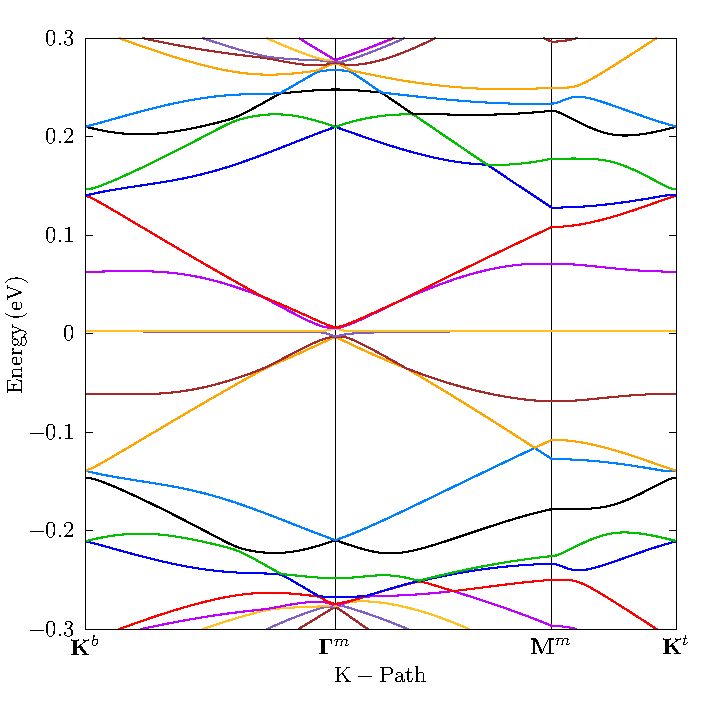
\includegraphics[width=0.5\linewidth]{pic/eb.pdf} 
    \caption{Energyband of TBG at \(\te = 1.05^\circ\)}
\end{figure}

\subsection{Hamiltonian in Real Space}
Now we give the derivation of Hamiltonian in real space. We start from \(p_{i} \rightarrow -i \partial_{i}\) where we suppress the constant \(\hbar\) and it gives the Hamiltonian in the top layer 
\begin{align}
	H_{top} = -i v_{F} \partial_{x} \p{\cos \frac\te2 \sigma_{x} - \sin \frac\te2 \sigma_{y}} - i v_{F} \partial_{y} \p{\sin \frac{\te}{2} \sigma_{x} + \cos \frac{\te}{2} \sigma_y},
\end{align}
where \(U\p{\te/2} = \exp(i \frac{\te}{4} \sigma_{z})\) and \(U\p{\te/2} \sigma_x U^{-1}\p{\te/2} =  \cos \frac{\te}{2} \sigma_{x} + \sin \frac{\te}{2} \sigma_{y}\). In the small-angle limit, we have \(\cos \frac{\te}{2} = 1,\, \sin \frac{\te}{2} = \frac{\te}{2}\). So the Hamiltonian in the top layer is
\begin{align}
	\begin{split}
		H_{top} & = -i v_{F} \partial_{x} \p{\sigma_x - \frac{\te}{2} \sigma_{y}} - i v_{F} \partial_{y} \p{\frac{\te}{2} \sigma_{x} + \sigma_{y}} \\
		& = -i v_F \p{\partial_{x} \sigma_{x} + \partial_{y} \sigma_{y}} - i v_{F} \frac{\te}{2} \p{-\partial_{x} \sigma_{y} - \partial_{y} \sigma_{x}} \\
		& \approx -i v_{F} \p{\partial_{\bm{r}} \cdot \hat{\sigma} - \frac{\te}{2} \partial_{\bm{r}} \times \hat{\sigma}}.
	\end{split}
\end{align}
We change the angle from \(\te/2\) to \(-\te/2\) for the bottom layer Hamiltonian:
\begin{align}
	H_{bottom}  = -i v_{F} \p{\partial_{\bm{r}} \cdot \hat{\sigma} + \frac{\te}{2} \partial_{\bm{r}} \times \hat{\sigma}}.
\end{align}

So we can rewrite the Hamiltonian in real space as
\begin{align}
	H  = \begin{pmatrix}
		H_{t} \p{\bm{r}} & T\p{\bm{r}} \\
		T^{\dagger} \p{\bm{r}} & H_{b} \p{\bm{r}},
	\end{pmatrix}
\end{align}
where 
\begin{align}
	H_{t/b} \p{\bm{r}} = -i v_{F} \p{\tau_0 \partial_{\bm{r}} \cdot \hat{\sigma} \mp \frac{\te}{2} \tau_z \partial_{\bm{r}} \times \hat{\sigma}},
\end{align}
and the interlayer coupling term is the moiré potential:
\begin{align}
	T\p{\bm{r}} = \sum_{i = 1}^{3} e^{-i \bm{q}_{i} \cdot \bm{r}} T_{i},
\end{align}
where \(\bm{q}_1 = 0,\, \bm{q}_2\)

\begin{itemize}
	\item momentum shift
\end{itemize}
Since \(\partial_{\bm{r}} \times \bm{\sigma} = \p{\partial_{\bm{r}} \times \bm{\sigma}} \cdot \hat{z}\) and \(\bm{A} \cdot \p{\bm{B} \times \bm{C}} = \p{\bm{A} \times \bm{B}} \cdot \bm{C} = \p{\bm{C} \times \bm{A}} \cdot \bm{B}\), we can rewrite this term as  
\begin{align}
	\p{\bm{k} \times \bm{\sigma}} \cdot \hat{z} = - \bm{\sigma} \cdot \p{\bm{k} \times \hat{z}},
\end{align}
and the Hamiltonian changed into 
\begin{align}
	H_{top} & \approx  v_{F} \hat{\sigma} \cdot \bm{k} - v_{F} \frac{\te}{2} \bm{k} \times \hat{\sigma} \\
	& = v_{F} \hat{\sigma} \cdot \bm{k} + v_{F} \frac{\te}{2} \bb{\hat{\sigma} \cdot \p{\bm{k} \times \hat{z}} } \\
	& = v_{F} \hat{\sigma} \cdot \bb{\bm{k} + \frac{\te}{2} \p{\bm{k} \times \hat{z}} }.
\end{align}
It is equivalent to a shift or more accurately, a rotation of the momentum \(\bm{k}\)

\begin{itemize}
	\item pseudomagnetic field
\end{itemize}
So the momentum shift in the top layer is \(\Delta \bm{k} = \frac{\te}{2} \p{\bm{k} \times \hat{z}}\) where \(\bm{k} \times \hat{z} = \p{k_{y}, - k_{x}}\). We need to write \(\bm{k} + \Delta \bm{k}\) as \(\bm{p} - \mr{e} \bm{A}\) or \(\bm{k} - \bm{A}_{eff}\), thus
\begin{align}
	\bm{A}_{eff}^{t} = - \Delta \bm{k} = - \frac{\te}{2} \p{\bm{k} \times \hat{z}} = - \frac{\te}{2} \begin{pmatrix}
		k_{y} \\
		- k_{x}
	\end{pmatrix}.		
\end{align}
For the bottom layer, the momentum shift is \(- \Delta \bm{k}\) and the effective vector potential is \(\bm{A}_{eff}^{b} = \frac{\te}{2} \p{\bm{k} \times \hat{z}}\) where 
\begin{align}
	\bm{A}_{eff}^{b} = - \bm{A}_{eff}^{t}.
\end{align}

We regarded the pseudomagnetic field as 
\begin{align}
	\bm{A}_{eff} = \bm{A}_{shift} + \bm{A}_{rot}.
\end{align}
and it protects the time-reversal symmetry.



\section{Symmetry}
\subsection{Formalism of symmetry}
We first specify the notations about symmetry and its representations. If the Hmailtonian is symmetric under a group operation, \(g\), we have 
\begin{align}
	H\p{g \bm{k}} = D_{\bm{k}} \p{g} H\p{\bm{k}} D_{\bm{k}} \p{g^{-1}},
\end{align}
where \(D_{\bm{k}}\) is the representation matrix of symmetry operator, in general depends on \(\bm{k}\).


Here we list several questions to answer what is the formalism of symmetry.

a. What is quantum transformation?

b. What is symmetry?

c. How do we  get the rotation center in the reciprocal lattice? and why \(\bm{\Gamma}\) is the only rotation center in the moire BZ(TBG) or FBZ(graphene)?

d. From the aspect of group representation theory, the representation matrix is the representation of rotation group under the basis of Bloch states. How to obtain the representation matrix?

e. Why can we still choose \(\bm{K}_{t}\) as the rotation center?


\subsection{\(C_{3z} \) Symmetry}

\begin{align}
	H \p{C_{3} \bm{k}} = U H \p{\bm{k}} U^{\dagger},
\end{align}
find out the matrix \(U\) or 
\begin{align} 
	\braket{C_{3z} \p{\bm{k}, A/B} | C_{3z}  \p{\bm{k}, A/B}}
\end{align}

For a state \(\ket{\bm{k}, \,\bm{K}^{t/b} + n_{1} \bm{b}^{m}_{1} + n_{2} \bm{b}^{m}_{2}}\), it is equivalent to \(\ket{\bm{k} - n_{1} \bm{b}^{m}_{1} - n_{2} \bm{b}^{m}_{2}, \, \bm{K}^{t/b},\, A/B}\). Consider the rotation occurs throughout the entire k-space, we set the origin at \(\bm{\Gamma}\) thus \(\p{\bm{k} - n_{1} \bm{b}^{m}_{1} - n_{2} \bm{b}^{m}_{2}} \rightarrow \p{\bm{K}^{t} + \bm{k} - n_{1} \bm{b}^{m}_{1} - n_{2}\bm{b}^{m}_{2}} \). The difference between \(\bm{K}^{t/b}\) and \(\bm{k} - n_{1} \bm{b}^{m}_{1} - n_{2}\bm{b}^{m}_{2}\) in the Bloch Hamiltonian changes into 
\begin{align}
	\p{\Delta \bm{k} }^{t/b} = \bm{K}^{t} + \bm{k} - n_{1} \bm{b}^{m}_{1} - n_{2}\bm{b}^{m}_{2} - \bm{K}^{t/b},
\end{align}
Under the \(C_{3z} \) rotation, the reciprocal lattice basis vectors change into 
\begin{align}
	C_{3z} \bm{b}^{m}_{1} = \bm{b}^{m}_{2}, \quad C_{3z} \bm{b}^{m}_{2} = - \p{ \bm{b}^{m}_{1} +  \bm{b}^{m}_{2}},
\end{align}
Thus 
\begin{align}
	\begin{split}
		C_{3z} \p{\Delta \bm{k} }^{t} = C_{3z} \bm{k} - n_{1} \bm{b}^{m}_{2} + n_{2} \p{ \bm{b}^{m}_{1} +  \bm{b}^{m}_{2}} = C_{3z} \bm{k} + n_{2} \bm{b}^{m}_{1} + \p{n_{2} - n_{1}}  \bm{b}^{m}_{2},
	\end{split}
\end{align}
and 
\begin{align}
	\begin{split}
		C_{3z} \p{\Delta \bm{k} }^{b} & = C_{3z} \p{\bm{K}^{t} + \bm{k} - n_{1} \bm{b}^{m}_{1} - n_{2}\bm{b}^{m}_{2} - \bm{K}^{t} - \bm{q}_{b}}  = C_{3z} \bm{k} - n_{1} \bm{b}^{m}_{2} + n_{2} \p{ \bm{b}^{m}_{1} +  \bm{b}^{m}_{2}} - \bm{q}_{tr} \\
		& = C_{3z} \bm{k} - n_{1} \bm{b}^{m}_{2} + n_{2} \p{ \bm{b}^{m}_{1} +  \bm{b}^{m}_{2}} - \p{\bm{q}_{b} + \bm{b}^{m}_{2}} \\
		& = C_{3z} \bm{k} + n_{2} \bm{b}^{m}_{1} + \p{n_{2} - n_{1} - 1}  \bm{b}^{m}_{2} - \bm{q}_{b}.
	\end{split}
\end{align}
For the position of atom \(\bm{r}_{A/B} = \bm{R} + \bm{\tau}_{A/B}\) after rotation
\begin{align}
	\begin{split}
		C_{3z} \bm{r}_{A} &= C_{3z} \p{\bm{R} + \bm{\tau}_{A}} = C_{3z} \bm{R} + \bm{\tau}_{A} \\
		C_{3z} \bm{r}_{B} &= C_{3z} \p{\bm{R} + \bm{\tau}_{B}} = C_{3z} \bm{R} + \frac{1}{3} \p{\bm{a}_{2} - 2 \bm{a}_{1}} \\
		& = C_{3z} \bm{R} + \bm{\tau}_{B} - \bm{a}_{1},
	\end{split}
\end{align}
and the new lattice vectors are
\begin{align}
		\bm{R}^{\prime}_{A} = C_{3z} \bm{R}_{A} ,\quad \bm{R}^{\prime}_{B} = C_{3z} \bm{R}_{B} - \bm{a}_{1}.
\end{align}

When we consider the top/bottom layer, the vectors \(\bm{a}_{1/2}\) and \(\bm{b}_{1/2}\) are actually \(\bm{a}^{t/b}_{1/2}\) and \(\bm{b}^{t/b}_{1/2}\) in the following derivation since we discussing the changes of the Bloch states within each layer after rotation. For the corresponding state in r-space \(\ket{\bm{R},\, t,\, A/B}\) where we choose the AA-aligned stacking and the Fourier transformation of the sublattice \(B\) is 
\begin{align}
	\begin{split}
		C_{3z} \ket{\bm{k} - n_{1} \bm{b}^{m}_{1} - n_{2} \bm{b}^{m}_{2}, \, \bm{K}^{t},\, B} & = \frac{1}{\sqrt{N_{1} N_{2}}} \sum_{\bm{R}} e^{i \p{\bm{K}^{t} + \bm{k} -n_{1} \bm{b}^{m}_{1} - n_{2} \bm{b}^{m}_{2}} \cdot \bm{R}} C_{3z} \ket{\bm{R}, t, B} \\
		& = \frac{1}{\sqrt{N_{1} N_{2}}} \sum_{\bm{R}} e^{i \p{\bm{K}^{t} + \bm{k} -n_{1} \bm{b}^{m}_{1} - n_{2} \bm{b}^{m}_{2}} \cdot \bm{R}} \ket{ C_{3z} \bm{R} - \bm{a}_{1}, t, B} \\
		& = \frac{1}{\sqrt{N_{1} N_{2}}} \sum_{\bm{k}} e^{i \p{\bm{K}^{t} + \bm{k} -n_{1} \bm{b}^{m}_{1} - n_{2} \bm{b}^{m}_{2}} \cdot C^{-1}_{3z} \p{\bm{R}^{\prime} + \bm{a}_{1}}} \ket{ \bm{R}^{\prime}, t, B} \\
		& = \frac{1}{\sqrt{N_{1} N_{2}}} \sum_{\bm{R}^\prime} e^{i C_{3z} \p{\bm{K}^{t} + \bm{k} -n_{1} \bm{b}^{m}_{1} - n_{2} \bm{b}^{m}_{2}} \cdot \p{\bm{R}^{\prime} + \bm{a}_{1}}} \ket{ \bm{R}^{\prime}, t, B} \\
		& = \frac{1}{\sqrt{N_{1} N_{2}}} \sum_{\bm{R}^\prime} e^{i \bb{C_{3z} \bm{K}^{t} + C_{3z} \bm{k} + n_{2} \bm{b}^{m}_{1} + \p{n_{2} - n_{1}} \bm{b}^{m}_{2}} \cdot \p{\bm{R}^{\prime} + \bm{a}_{1}}} \ket{ \bm{R}^{\prime}, t, B} \\
		& \approx  \frac{1}{\sqrt{N_{1} N_{2}}} \sum_{\bm{R}^\prime} e^{i \bb{\bm{K}^{t} + \bm{b}_{2} + C_{3z} \bm{k} + n_{2} \bm{b}^{m}_{1} + \p{n_{2} - n_{1}} \bm{b}^{m}_{2}} \cdot \p{\bm{R}^{\prime} + \bm{a}_{1}}} \ket{ \bm{R}^{\prime}, t, B} \\
		& = \frac{1}{\sqrt{N_{1} N_{2}}} \sum_{\bm{R}^\prime} e^{i \bm{b}_{2} \cdot \p{\bm{R}^{\prime} + \bm{a}_{1}}} e^{i \bb{\bm{K}^{t} + C_{3z} \bm{k} + n_{2} \bm{b}^{m}_{1} + \p{n_{2} - n_{1}} \bm{b}^{m}_{2}} \cdot \p{\bm{R}^{\prime} + \bm{a}_{1}}} \ket{ \bm{R}^{\prime}, t, B} \\
		& = \frac{1}{\sqrt{N_{1} N_{2}}} \sum_{\bm{R}^\prime} e^{i \bb{\bm{K}^{t} + C_{3z} \bm{k} + n_{2} \bm{b}^{m}_{1} + \p{n_{2} - n_{1}} \bm{b}^{m}_{2}} \cdot \p{\bm{R}^{\prime} + \bm{a}_{1}}} \ket{ \bm{R}^{\prime}, t/b, B} \\
		& = \frac{1}{\sqrt{N_{1} N_{2}}} \sum_{\bm{R}^\prime} e^{i \bb{\bm{K}^{t} + C_{3z} \bm{k} + n_{2} \bm{b}^{m}_{1} + \p{n_{2} - n_{1}} \bm{b}^{m}_{2}} \cdot \bm{R}^{\prime} }  e^{i \bb{\bm{K}^{t} + C_{3z} \bm{k} + n_{2} \bm{b}^{m}_{1} + \p{n_{2} - n_{1}} \bm{b}^{m}_{2}} \cdot \bm{a}_{1}} \ket{ \bm{R}^{\prime}, t, B} \\
		& = \frac{1}{\sqrt{N_{1} N_{2}}} \sum_{\bm{R}^\prime} e^{i \bm{K}^{t} \cdot \bm{a}_{1}} e^{i \bb{\bm{K}^{t} + C_{3z} \bm{k} + n_{2} \bm{b}^{m}_{1} + \p{n_{2} - n_{1}} \bm{b}^{m}_{2}} \cdot \bm{R}^{\prime} } \ket{ \bm{R}^{\prime}, t, B} \\
		& = e^{i \bm{K}^{t} \cdot \bm{a}_{1}} \ket{C_{3z} \bm{k} +n_{2} \bm{b}^{m}_{1} + \p{n_{2} - n_{1}} \bm{b}^{m}_{2}, \bm{K}^{t}, B} 
	\end{split}
\end{align}
where we neglect small term since \(\bm{K}^{t} \gg \bm{k}, \bm{b}^{m}_{1},  \bm{b}^{m}_{2}\)(but actually it is rigorous since we can consider it as a translation applied to the Bloch state) and with the following realtions.
\begin{align}
	\begin{split}
		C_{3z}  \bm{K}^{t}  & =  \bm{K}^{t} + \bm{b}_{2} \\
		\bm{b}_{2} \cdot \p{\bm{R}^{\prime} + \bm{a}_{2}} &= 2N \pi, \quad N \in \mathbb{Z}.
	\end{split}
\end{align}
For sublattice \(A\)
\begin{align}
	C_{3z} \ket{\bm{k} - n_{1} \bm{b}^{m}_{1} - n_{2} \bm{b}^{m}_{2}, \, \bm{K}^{t},\, A}  = \ket{C_{3z} \bm{k} +n_{2} \bm{b}^{m}_{1} + \p{n_{2} - n_{1}} \bm{b}^{m}_{2}, \bm{K}^{t}, A}.
\end{align}
which is 
\begin{align}
	C_{3z} \ket{\bm{k} - n_{1} \bm{b}^{m}_{1} - n_{2} \bm{b}^{m}_{2}, \, \bm{K}^{t}} = \begin{bmatrix}
		1 & \\ 
		 & e^{\frac{2}{3} \pi i}
	\end{bmatrix} \ket{C_{3z} \bm{k} +n_{2} \bm{b}^{m}_{1} + \p{n_{2} - n_{1}} \bm{b}^{m}_{2}, \bm{K}^{t}}.
\end{align}
If the layer index changes into \(\bm{K}^{b}\), the new state is 
\begin{align}
		C_{3z} \ket{\bm{k} - n_{1} \bm{b}^{m}_{1} - n_{2} \bm{b}^{m}_{2}, \, \bm{K}^{b}}  & = \begin{bmatrix}
			1 & \\ 
			 & e^{\frac{2}{3} \pi i}
		\end{bmatrix} \ket{C_{3z} \bm{k} +n_{2} \bm{b}^{m}_{1} + \p{n_{2} - n_{1} -1} \bm{b}^{m}_{2}, \bm{K}^{b}}.
\end{align}

Now we need to check the Hamiltonian matrix elements is invariant under the \(C_{3z}\) rortation, which is 
\begin{align}
	\braket{\psi|\hat{H}|\phi} = \braket{C_{3z} \psi | \hat{H} | C_{3z}  \phi} = \braket{\psi| C^{\dagger}_{3z} \hat{H} C_{3z} | \phi}.
\end{align}
The diagonal term of top layer after rotation is
\begin{align}
	\begin{split}
		& \braket{\bm{k} -n_{1} \bm{b}^{m}_{1} - n_{2} \bm{b}^{m}_{2}, \bm{K}^{t}|C^{\dagger}_{3z} \hat{H} C_{3z}|\bm{k} -n_{1} \bm{b}^{m}_{1} - n_{2} \bm{b}^{m}_{2}, \bm{K}^{t}} \\
		& =  \begin{bmatrix}
			1 & \\ 
			 & e^{ - \frac{2}{3} \pi i}
		\end{bmatrix} \braket{C_{3z}\bm{k} + n_{2} \bm{b}^{m}_{1} + \p{n_{2} - n_{1}} \bm{b}^{m}_{2}, \bm{K}^{t}| \hat{H} |C_{3z} \bm{k} + n_{2} \bm{b}^{m}_{1} + \p{n_{2} - n_{1} }\bm{b}^{m}_{2}, \bm{K}^{t}}  \begin{bmatrix}
			1 & \\ 
			 & e^{\frac{2}{3} \pi i}
		\end{bmatrix} \\
		& = \begin{bmatrix}
			1 & \\ 
			 & e^{ - \frac{2}{3} \pi i}
		\end{bmatrix} v_{F} \hbar \bb{C_{3z} \bm{k} + n_{2} \bm{b}^{m}_{1} + \p{n_{2} - n_{1} }\bm{b}^{m}_{2}} \cdot \sigma^{\te^\prime/2} \begin{bmatrix}
			1 & \\ 
			 & e^{i \frac{2}{3} \pi}
		\end{bmatrix} \\
		& = v_{F} \hbar |C_{3z} \p{\bm{k} - n_{1} \bm{b}^{m}_{1} - n_{2} \bm{b}^{m}_{2}} | \cdot \begin{bmatrix}
			1 & \\ 
			 & e^{ - i \frac{2}{3} \pi }
		\end{bmatrix} \begin{bmatrix}
			0 & e^{-i \p{\te_{\bm{k}} + \frac{2}{3}\pi - \frac{\te}{2}}} \\
			e^{i \p{\te_{\bm{k}} + \frac{2}{3}\pi - \frac{\te}{2}}} & 0
		\end{bmatrix} \begin{bmatrix}
			1 & \\ 
			 & e^{i \frac{2}{3} \pi}
		\end{bmatrix} \\
		& = v_{F} \hbar \, |C_{3z} \p{\bm{k} - n_{1} \bm{b}^{m}_{1} - n_{2} \bm{b}^{m}_{2}} | \cdot \begin{bmatrix}
			0 & e^{-i \p{\te_{\bm{k}} - \frac{\te}{2}}} \\
			e^{i \p{\te_{\bm{k}} - \frac{\te}{2}}} & 0
		\end{bmatrix} \\
		& = v_{F} \hbar |C_{3z} \p{\bm{k} - n_{1} \bm{b}^{m}_{1} - n_{2} \bm{b}^{m}_{2}} | \cdot \sigma_{\te/2} \\
		&=\braket{\bm{k} -n_{1} \bm{b}^{m}_{1} - n_{2} \bm{b}^{m}_{2}, \bm{K}^{t}|\hat{H}|\bm{k} -n_{1} \bm{b}^{m}_{1} - n_{2} \bm{b}^{m}_{2}, \bm{K}^{t}}
	\end{split}
\end{align}
where \(|C_{3z} \p{\bm{k} - n_{1} \bm{b}^{m}_{1} - n_{2} \bm{b}^{m}_{2}} | = |\bm{k} - n_{1} \bm{b}^{m}_{1} - n_{2} \bm{b}^{m}_{2}|\) and the diagonal term of bottom layer can be verified in the same way. 
For the off-diagonal terms, \(\braket{\bm{k}, \bm{K}^{b} + n_{1} \bm{b}^{m}_{1} + n_{2} \bm{b}^{m}_{2}| \hat{H}|\bm{k}, \bm{K}^{t} + m_{1} \bm{b}^{m}_{1} + m_{2} \bm{b}^{m}_{2} }\) changes into
\begin{align}
	\braket{C_{3 z} \bm{k} - \p{-n_{2}} \bm{b}^{m}_{1} - \p{n_{1} - n_{2} + 1} \bm{b}^{m}_{2}, \bm{K}^{b}|\hat{H} |C_{3 z} \bm{k} - \p{-m_{2}} \bm{b}^{m}_{1} - \p{m_{1} - m_{2}} \bm{b}^{m}_{2}, \bm{K}^{t} },
\end{align}
thus if \(n_{1} = m_{1}, n_{2} = m_{2}\)
\begin{align}
	- n_{2} = - m_{2},\quad n_{1} - n_{2} + 1 = m_{1} - m_{2} + 1,
\end{align}
which leads to 
\begin{align}
	\braket{C_{3 z} \bm{k} - \p{-n_{2}} \bm{b}^{m}_{1} - \p{n_{1} - n_{2} + 1} \bm{b}^{m}_{2}, \bm{K}^{b}|\hat{H} |C_{3 z} \bm{k} - \p{-m_{2}} \bm{b}^{m}_{1} - \p{m_{1} - m_{2}} \bm{b}^{m}_{2}, \bm{K}^{t} } = T_{\bm{q}_{tr}}.
\end{align}
If \(n_{1} = m_{1}, n_{2} = m_{2} + 1\) 
\begin{align}
	- n_{2} = -m_{2}  - 1 ,\quad n_{1} - n_{2} + 1 = m_{1} - m_{2},
\end{align}
which leads to
\begin{align}
	\braket{C_{3 z} \bm{k} - \p{-n_{2}} \bm{b}^{m}_{1} - \p{n_{1} - n_{2} + 1} \bm{b}^{m}_{2}, \bm{K}^{b}|\hat{H} |C_{3 z} \bm{k} - \p{-m_{2}} \bm{b}^{m}_{1} - \p{m_{1} - m_{2}} \bm{b}^{m}_{2}, \bm{K}^{t} } = T_{\bm{q}_{tl}}.
\end{align}
More generally
\begin{align}
	\braket{C_{3 z} \bm{k} + n_{2} \bm{b}^{m}_{1} + \p{n_{2} - n_{1} -1} \bm{b}^{m}_{2}, \bm{K}^{b}|\hat{H} |C_{3 z} \bm{k}+  m_{2} \bm{b}^{m}_{1} + \p{m_{2} - m_{1}} \bm{b}^{m}_{2}, \bm{K}^{t} } =  \begin{cases}
		&T_{\bm{q}_{tr}} ,\quad n_1 = m_1,\, n_2 = m_2 \\
		&T_{\bm{q}_{tl}}, \quad n_1 = m_1,\, n_2 = m_2 +1 \\
		&T_{\bm{q}_{b}}, \quad n_1 = m_1-1,\, n_2 = m_2
	\end{cases},
\end{align}
where a corresponding rotation change also occurs for the matrix
\begin{align}
	T_{\bm{q}_{b}} \rightarrow T_{\bm{q}_{tr}}, \quad T_{\bm{q}_{tr}} \rightarrow T_{\bm{q}_{tl}}, \quad T_{\bm{q}_{tl}} \rightarrow T_{\bm{q}_{b}}.
\end{align}

For the tripod model, the \(8 \times 8\) matrix should be
\begin{align}
	U = 
	\begin{pmatrix}
		A & 0 & 0 & 0 \\
		0 & 0 & 0 & A \\
		0 & A & 0 & 0 \\
		0 & 0 & A & 0
	\end{pmatrix}, \quad A = \begin{pmatrix}
		1 & 0 \\
		0 & e^{i\frac{2 \pi}{3}}
	\end{pmatrix}.
\end{align}
since the state changes under the \(C_{3z}\) rotation is
\begin{align}
	\begin{pmatrix}
		\ket{\psi_{1}} \\ \ket{\psi_{2}} \\ \ket{\psi_{3}} \\ \ket{\psi_{4}} 
	\end{pmatrix} \rightarrow \begin{pmatrix}
		\ket{\psi_{1}} \\ \ket{\psi_{4}} \\ \ket{\psi_{3}} \\ \ket{\psi_{2}} 
	\end{pmatrix} 
\end{align}
where the matrix \(U\) satisfies \(U^{\dagger} H U = H,\quad U^\dagger U = I\). The matrix \(A\) can be rewritten as 
\begin{align}
	A  = \begin{pmatrix}
		e^{-i \pi/3} & 0 \\
		0 & e^{i \pi/3}
	\end{pmatrix},
\end{align}
since the phase \(e^{i \pi/3}\)  is meaningless.


\subsection{$C_{2z} \mathcal{T} $ Symmetry}
Before we discuss the \(C_{2z} \mathcal{T}\) symmetry in TBG, we need to clarify the time reversal symmetry \(\mathcal{T}\) and the \(C_{2z}\) symmetry in graphene. The time reversal symmetry asks
\begin{align}
	\bb{\mathcal{T}, H} = 0 \quad \mr{or} \quad \mathcal{T} H \mathcal{T}^{-1} = H,
\end{align}
Here it should be in the form of operators but we neglect it since what we really care is the relation between \(\mathcal{T}\) and Bloch Hamiltonian \(h\p{\bm{k}}\). Following the derivation in Bernevig's book, we have 
\begin{align}
	\mathcal{T} \hat{c}_{\bm{r}} \mathcal{T}^{-1} = \hat{c}_{\bm{r}},
\end{align}
and correspondingly 
\begin{align}
	\mathcal{T} \hat{c}_{\bm{r}} \mathcal{T}^{-1} = \mathcal{T} \frac{1}{\sqrt{N}} \sum_{\bm{k}} e^{i \bm{k} \cdot \bm{r}} \hat{c}_{\bm{k}} \mathcal{T}^{-1} = \frac{1}{\sqrt{N}} \sum_{\bm{k}} e^{ - i \bm{k} \cdot \bm{r}} \mathcal{T} \hat{c}_{\bm{k}} \mathcal{T}^{-1} = \frac{1}{\sqrt{N}} \sum_{\bm{k}} e^{ - i \bm{k} \cdot \bm{r}} \hat{c}_{- \bm{k}}.
\end{align}
where the action of \(\mathcal{T}\) on the momentum operator is to flip the sign of the momentum, i.e., \(\mathcal{T} \hat{c}_{\bm{k}} \mathcal{T}^{-1} = \hat{c}_{- \bm{k}}\). Thus we have
\begin{align}
	\mathcal{T} \hat{H} \mathcal{T}^{-1} = \sum_{\bm{k}} \hat{c}^\dagger_{-\bm{k}} \mathcal{T} h\p{\bm{k}} \mathcal{T}^{-1} \hat{c}_{-\bm{k}} = \hat{H} = \sum_{\bm{k}} \hat{c}^\dagger_{\bm{k}} h\p{\bm{k}} \hat{c}_{\bm{k}} = \sum_{\bm{k}} \hat{c}_{- \bm{k}} h \p{- \bm{k}} \hat{c}^\dagger_{- \bm{k}},
\end{align}
which is 
\begin{align}
	\boxed{\mathcal{T} h\p{\bm{k}} \mathcal{T}^{-1} = h\p{- \bm{k}}}.
\end{align}
In graphene, electrons are usually regarded as spinless fermions since we completely neglect the spin-orbit coupling(\(\mu \mr{eV}\) scale). Thus the time reversal symmetry is simply \(\mathcal{T} = \mathcal{K}\), where \(\mathcal{K}\) is the complex conjugation operator. So 
\begin{align}
	\boxed{h^* \p{\bm{k}} = h\p{- \bm{k}}}.
\end{align}
For the \(C_{2z}\) symmetry or inversion symmetry, we assume the rotation respect to the middle of the primetive cell where \(C_{2z} \bm{r} = - \bm{r}\) and 
\begin{align}
	C_{2z} \hat{c}_{\bm{R};A} C_{2z}^{-1} = \hat{c}_{-\bm{R};B},\quad C_{2z} \hat{c}_{\bm{R};B} C_{2z}^{-1} = \hat{c}_{-\bm{R};A},
\end{align}


For the state \(\ket{\bm{k} -n_{1} \bm{b}^{m}_{1} - n_{2} \bm{b}^{m}_{2}, \bm{K}^{t}, B}\), time revesal symmetry \(\mathcal{T}\) gives 
\begin{align}
	\begin{split}
		\mathcal{T}\ket{\bm{k} -n_{1} \bm{b}^{m}_{1} - n_{2} \bm{b}^{m}_{2}, \bm{K}^{t}, B} & = \mathcal{T} \frac{1}{\sqrt{N_1 N_{2}}} \sum_{\bm{R}} e^{i \p{\bm{K}^{t} + \bm{k} - n_{1} \bm{b}^{m}_{1} - n_{2} \bm{b}^{m}_{2}} \cdot \bm{R}} \ket{\bm{R}, t, B} \\
		& = \frac{1}{\sqrt{N_1 N_{2}}} \sum_{\bm{R}} e^{- i \p{\bm{K}^{t} + \bm{k} - n_{1} \bm{b}^{m}_{1} - n_{2} \bm{b}^{m}_{2}} \cdot \bm{R}} \mathcal{T} \ket{\bm{R}, t, B} \\
		& = \frac{1}{\sqrt{N_1 N_{2}}} \sum_{\bm{R}} e^{ i \p{ - \bm{K}^{t} - \bm{k} + n_{1} \bm{b}^{m}_{1} + n_{2} \bm{b}^{m}_{2}} \cdot \bm{R}} \ket{\bm{R}, t, B} \\
		& = \ket{ - \bm{k} + n_{1} \bm{b}^{m}_{1} + n_{2} \bm{b}^{m}_{2}, - \bm{K}^{t}, B}.
	\end{split}
\end{align}
For \(C_{2z}\) symmetry, we assume the rotation center in real space is \(\p{0,\frac{a}{2\sqrt{3}}}\), thus 
\begin{align}
	\begin{split}
		C_{2z} \bm{r}_{A} &= C_{2z} \p{\bm{R} + \bm{\tau}_{A}} = C_{2z} \bm{R} + \bm{\tau}_{B} \\
	C_{2z} \bm{r}_{B}& = C_{2z} \p{\bm{R} + \bm{\tau}_{B}} = C_{2z} \bm{R} + \bm{\tau}_{A}.
	\end{split}
\end{align}
The corresponding momenta are 
\begin{align}
	C_{2z} \p{\bm{k} + \bm{K}^{t/b} - n_{1} \bm{b}^{m}_{1} - n_{2} \bm{b}^{m}_{2}} = - \bm{k} - \bm{K}^{t/b} + n_{1} \bm{b}^{m}_{1} + n_{2} \bm{b}^{m}_{2},
\end{align}
which leads to 
\begin{align}
	\begin{split}
		C_{2z} \mathcal{T}\ket{\bm{k} -n_{1} \bm{b}^{m}_{1} - n_{2} \bm{b}^{m}_{2}, \bm{K}^{t}, B} & = C_{2z}  \ket{ - \bm{k} + n_{1} \bm{b}^{m}_{1} + n_{2} \bm{b}^{m}_{2}, - \bm{K}^{t}, B} \\
		& = \frac{1}{\sqrt{N_{1} N_{2}}} \sum_{\bm{R}} e^{ i \p{ - \bm{K}^{t} - \bm{k} + n_{1} \bm{b}^{m}_{1} + n_{2} \bm{b}^{m}_{2}} \cdot \bm{R}} C_{2z} \ket{\bm{R}, t, B} \\
		& = \frac{1}{\sqrt{N_{1} N_{2}}} \sum_{\bm{R}} e^{ i \p{ - \bm{K}^{t} - \bm{k} + n_{1} \bm{b}^{m}_{1} + n_{2} \bm{b}^{m}_{2}} \cdot C^{-1}_{2z} \bm{R}^\prime}  \ket{\bm{R}^\prime, t, A} \\
		& =  \frac{1}{\sqrt{N_{1} N_{2}}} \sum_{\bm{R}} e^{ i C_{2z} \p{ - \bm{K}^{t} - \bm{k} + n_{1} \bm{b}^{m}_{1} + n_{2} \bm{b}^{m}_{2}} \cdot \bm{R}^\prime}  \ket{\bm{R}^\prime, t, A} \\
		& =  \frac{1}{\sqrt{N_{1} N_{2}}} \sum_{\bm{R}} e^{ i \p{\bm{K}^{t} + \bm{k} - n_{1} \bm{b}^{m}_{1} - n_{2} \bm{b}^{m}_{2}} \cdot \bm{R}^\prime}  \ket{\bm{R}^\prime, t, A} \\
		& = \ket{\bm{k} -n_{1} \bm{b}^{m}_{1} - n_{2} \bm{b}^{m}_{2}, \bm{K}^{t}, A}.
	\end{split}
\end{align}
More generally, 
\begin{align}
	C_{2z} \mathcal{T}\ket{\bm{k} -n_{1} \bm{b}^{m}_{1} - n_{2} \bm{b}^{m}_{2}, \bm{K}^{t}, A/B} = \begin{bmatrix}
		0 & 1 \\
		1 & 0 
	\end{bmatrix} \ket{\bm{k} -n_{1} \bm{b}^{m}_{1} - n_{2} \bm{b}^{m}_{2}, \bm{K}^{t}, A/B},
\end{align}
Thus  
\begin{align}
	\begin{split}
		&\braket{C_{2z} \mathcal{T} \p{\bm{k} -n_{1} \bm{b}^{m}_{1} - n_{2} \bm{b}^{m}_{2}, \bm{K}^{t}} | \hat{H} | C_{2z} \mathcal{T} \p{\bm{k} -n_{1} \bm{b}^{m}_{1} - n_{2} \bm{b}^{m}_{2}, \bm{K}^{t}}} \\
		&= \braket{\bm{k} -n_{1} \bm{b}^{m}_{1} - n_{2} \bm{b}^{m}_{2}, \bm{K}^{t} | \hat{H} | \bm{k} -n_{1} \bm{b}^{m}_{1} - n_{2} \bm{b}^{m}_{2}, \bm{K}^{t}}^{*}.
	\end{split}
\end{align}

\(C_{2z} \mathcal{T} \) exchanges the sublattice, but does not change the momentum. In general, we can write \(C_{2z} \mathcal{T} \) as
\begin{align}
	H_{2 \times 2} \p{\bm{k}}= \sigma_{x} H^{*}_{2 \times 2}  \p{\bm{k}} \sigma_{x}. 
\end{align}
and the time reversal operator is
\begin{align}
	\Theta = D K, \quad D =\begin{pmatrix}
		\sigma_{x} & &   \\
		& \sigma_{x} &  \\
		& & \ddots
	\end{pmatrix}.
\end{align}
where \(\mathcal{K}\) is the complex conjugate operator and the \(C_{2z} \mathcal{T} \) can be experessed as 
\begin{align}
	H \p{\bm{k}} = D^\dagger H^{*} \p{\bm{k}} D.
\end{align}

\subsection{$C_{2 x}$ Symmetry}
For \(C_{2x}\) rotation, we have 
\begin{align}
	\begin{split}
		C_{2x} \bm{r}_{A} &= C_{2x} \p{\bm{R} + \bm{\tau}_{A}} = C_{2x} \bm{R} + \bm{\tau}_{B} \\
		C_{2x} \bm{r}_{B} &= C_{2x} \p{\bm{R} + \bm{\tau}_{B}} = C_{2x} \bm{R} + \bm{\tau}_{A}.
	\end{split}
\end{align} 
and 
\begin{align}
	C_{2x} \bm{a}_{1} = a \p{\frac{1}{2}, -\frac{\sqrt{3}}{2}},\quad C_{2x} \bm{a}_{2} = a \p{-\frac{1}{2}, -\frac{\sqrt{3}}{2}}.
\end{align}
In k-space
\begin{align}
	C_{2z} \bm{b}^{m}_{1} = \bm{b}^{m}_{2}, \quad C_{2z} \bm{b}^{m}_{2} = \bm{b}^{m}_{1},
\end{align}
and 
\begin{align}
	C_{2x} \bm{K}^{t} = \bm{K}^{b} ,\quad C_{2x} \bm{K}^{b} = \bm{K}^{t}.
\end{align}
Thus 
\begin{align}
	\begin{split}
		C_{2x} \ket{\bm{k} -n_{1} \bm{b}^{m}_{1} - n_{2} \bm{b}^{m}_{2}, \bm{K}^{t}, t, B} & = \frac{1}{\sqrt{N_1 N_{2}}} \sum_{\bm{R}} e^{i \p{\bm{K}^{t} + \bm{k} - n_{1} \bm{b}^{m}_{1} - n_{2} \bm{b}^{m}_{2}} \cdot \bm{R} } C_{2x} \ket{\bm{R}, t, B} \\
		& = \frac{1}{\sqrt{N_1 N_{2}}} \sum_{\bm{R}} e^{i \p{\bm{K}^{t} + \bm{k} - n_{1} \bm{b}^{m}_{1} - n_{2} \bm{b}^{m}_{2}} \cdot \bm{R} }  \ket{C_{2x} \bm{R}, t, A} \\ 
		& = \frac{1}{\sqrt{N_1 N_{2}}} \sum_{\bm{R}^\prime} e^{i \p{\bm{K}^{t} + \bm{k} - n_{1} \bm{b}^{m}_{1} - n_{2} \bm{b}^{m}_{2}} \cdot C^{-1}_{2x}\bm{R}^\prime }  \ket{ \bm{R}^\prime, t, A} \\
		& = \frac{1}{\sqrt{N_1 N_{2}}} \sum_{\bm{R}^\prime} e^{i  \bb{C_{2x} \p{\bm{K}^{t} + \bm{k} - n_{1} \bm{b}^{m}_{1} - n_{2} \bm{b}^{m}_{2}}} \cdot \bm{R}^\prime }  \ket{ \bm{R}^\prime, t, A} \\
		& = \frac{1}{\sqrt{N_1 N_{2}}} \sum_{\bm{R}^\prime} e^{i \p{C_{2x} \bm{k} + \bm{K}^{b} - n_{1} \bm{b}^{m}_{2} - n_{2} \bm{b}^{m}_{1}} \cdot \bm{R}^\prime }  \ket{ \bm{R}^\prime, t, A} \\
		& = \ket{C_{2x} \bm{k}- n_{2} \bm{b}^{m}_{1} - n_{1} \bm{b}^{m}_{2} , \bm{K}^{b}, t, A}.
	\end{split}
\end{align}
More generally,
\begin{align}
	C_{2x} \ket{\bm{k} -n_{1} \bm{b}^{m}_{1} - n_{2} \bm{b}^{m}_{2}, \bm{K}^{t}, t, A/B} = \begin{bmatrix}
		0 & 1 \\
		1 & 0
	\end{bmatrix} \ket{C_{2x} \bm{k}- n_{2} \bm{b}^{m}_{1} - n_{1} \bm{b}^{m}_{2} , \bm{K}^{b}, t, A/B }.
\end{align}


\subsection{Particle-Hole Symmetry}
The particle-hole symmetry at \(\bm{K}^{t}\) satisfies
\begin{align}
	\hat{V}^{\dagger} \hat{H} \hat{V} = - \hat{H},
\end{align}
In tripod model, the unitary and Hermitian matrix is 
\begin{align}
	V = \begin{pmatrix}
		-\sigma_{x} & 0 & 0 & 0 \\
		0 & \sigma_{x} & 0 & 0 \\
		0 & 0 & 0 & \sigma_{x} \\
		0 & 0 & \sigma_{x} & 0
	\end{pmatrix}.
\end{align}
Actually, the particle-hole symmetry is 
\begin{align}
	V^\dagger H(\bm{k}) V = - H(-\bm{k}).
\end{align}
\\
Symmetry on flat band at $\mathbf{K}^{t}$: \textcolor{red}{\(C_{3z} \rightarrow \bm{k} = 0\),  \( C_{2z} \mathcal{T} \rightarrow\) degeneracy, PH symmetry \(\rightarrow E = 0\) }



\section{Eigenstates}
Assuming the two degenerate states of the zero band at \(\bm{K}^{t}\) are \(\ket{\psi_{1}}\) and \(\ket{\psi_{2}}\). It is obvious that the linear combination of \(\ket{\psi_{1}}\) and \(\ket{\psi_{2}}\) is also the eigenstate of zero band which is 
\begin{align}
	\hat{H} \p{\alpha \ket{\psi_{1}} + \beta \ket{\psi_{2}} } = 0 \p{\alpha \ket{\psi_{1}} + \beta \ket{\psi_{2}} }.
\end{align}
So it is meaningless to determine \(\ket{\psi_{1}}\) and \(\ket{\psi_{2}}\). But if there is a unitary matrix \(U\) it has two different non-degenerate eigenvalues under the basis \(\ket{\psi_{1}}\) and \(\ket{\psi_{2}}\), the correspondingly eigenstates \(\ket{\phi_{1}}\) and \(\ket{\phi_{2}}\) are certain since the diemension of eigenspace is 1 for each eigenvalue(only phase difference).  

The problem changes into to figure out \(\ket{\phi_{1}}\) and \(\ket{\phi_{2}}\).(The following text we have mixed the use of \(\ket{\ph}\) and \(\ph\)) 

\subsection{Tripod Model}
We diagonlize unitary matrix of \(C_{3z}\) in the Hilbert space with the basis \(\ket{\psi_{1}}\) and \(\ket{\psi_{2}}\) and get the eigenstates composed of \(\ket{\psi_{1}}\) and \(\ket{\psi_{2}}\) linear combination when \(w_0 = w_1\)

\begin{align}
	\begin{split}
		\ket{\phi_{1}} & = \frac{\sqrt{2}}{2} \ket{\psi_{1}} + \frac{\sqrt{2}i}{2} \ket{\psi_{2}} \\
		\ket{\phi_{2}} & = \frac{\sqrt{2}i}{2} \ket{\psi_{1}} + \frac{\sqrt{2}}{2} \ket{\psi_{2}},
	\end{split}
\end{align}
and the coefficient matrix will change if \(w_0 \neq w_1\). The corresponding eigenvalues are \(e^{i \frac{\pi}{3}} \) and \(e^{- i \frac{\pi}{3} }\) which can be obtianed numerically. So the eigenequation for \(e^{i \frac{\pi}{3}}\) is
\begin{align}
	\begin{pmatrix}
		A \phi_{11} \\  A \phi_{14} \\ A \phi_{12} \\ A \phi_{13}
	\end{pmatrix} = e^{i \frac{\pi}{3}} \begin{pmatrix}
		\phi_{11} \\ \phi_{12} \\ \phi_{13} \\ \phi_{14}
	\end{pmatrix},
\end{align}
which leads to \(\phi_{11} = \alpha \begin{pmatrix}
	0 \\ 1
\end{pmatrix}\)
and 
\begin{align}
	\begin{split}
		&\phi_{12}^{B} = \phi_{13}^{B} = \phi_{14}^{B} \\
		&\phi_{13}^{A} = e^{-i\frac{2 \pi}{3}} \phi_{12}^{A}, \quad \phi_{14}^{A} = e^{i\frac{2 \pi}{3}} \phi_{12}^{A}.
	\end{split}
\end{align}
Similarily, the eigenequation for \(e^{-i \frac{\pi}{3}}\) is
\begin{align}
	\begin{pmatrix}
		A \phi_{21} \\  A \phi_{24} \\ A \phi_{22} \\ A \phi_{23}
	\end{pmatrix} = e^{-i \frac{\pi}{3}} \begin{pmatrix}
		\phi_{21} \\ \phi_{22} \\ \phi_{23} \\ \phi_{24}
	\end{pmatrix},
\end{align}
thus \(\phi_{21} = \beta \begin{pmatrix}
	1 \\ 0	
\end{pmatrix}\)
and
\begin{align}
	\begin{split}
		&\phi_{22}^{A} = \phi_{23}^{A} = \phi_{24}^{A} \\
		&\phi_{23}^{B} = e^{i\frac{2 \pi}{3}} \phi_{22}^{B}, \quad \phi_{24}^{B} = e^{- i\frac{2 \pi}{3}} \phi_{22}^{B}.
	\end{split}
\end{align}
We set \(\Phi = \begin{pmatrix}
	\phi_{1} & \phi_{2}
\end{pmatrix}\) and the representation matrix of particle-hole symmetry under \(\ph_1\) and \(\ph_2\) when \(w_0 = w_1\)is 
\begin{align}
	\braket{\Phi | V | \Phi} = 
	\begin{pmatrix}
		0 & -1 \\ -1 & 0
	\end{pmatrix}
\end{align}
The eigenstates of unitary matrix of particle-hole symmetry are
\begin{align}
	\begin{split}
		\ket{\phi^\prime_{1}} & =   \frac{\sqrt{2}}{2} \ket{\phi_{1}} + \frac{\sqrt{2}}{2} \ket{\phi_{2}} \\
		\ket{\phi^\prime_{2}} & =   - \frac{\sqrt{2}}{2} \ket{\phi_{1}} + \frac{\sqrt{2}}{2} \ket{\phi_{2}},
	\end{split}
\end{align}
and the eigenvalues are \(-1\) and \(1\). We need to ponit out that the representation matrix will change from if \(w_0 \neq w_1\)
\begin{align}
	\begin{pmatrix}
		0 & -1 \\ -1 & 0
	\end{pmatrix} \rightarrow \begin{pmatrix}
		0 & e^{i \te} \\ e^{-i \te} & 0 
	\end{pmatrix},
\end{align}
and actually \(e^{i \te}\) is the phase factor without any physical meaning but we might guess the determinant of the representation matrix is \(-1\) (we will prove it later). The eigenequation for \(-1\) is
\begin{align}
	\begin{pmatrix}
		-\sigma_{x} \p{ \phi_{11} +  \phi_{21}} \\  \sigma_{x} \p{\phi_{12} + \phi_{22}} \\ \sigma_{x} \p{\phi_{14} + \phi_{24}} \\ \sigma_{x} \p{\phi_{13} + \phi_{23}}
	\end{pmatrix} = - \begin{pmatrix}
		\phi_{11} + \phi_{21} \\ \phi_{12} + \phi_{22} \\ \phi_{13} + \phi_{23} \\ \phi_{14} + \phi_{23}
	\end{pmatrix},
\end{align}
where we omit the coefficient \(\sqrt{2}/2\) and the eigenequation for \(1\) is
\begin{align}
	\begin{pmatrix}
		-\sigma_{x} \p{ - \phi_{11} +  \phi_{21}} \\  \sigma_{x} \p{ - \phi_{12} + \phi_{22}} \\ \sigma_{x} \p{ - \phi_{14} + \phi_{24}} \\ \sigma_{x} \p{ - \phi_{13} + \phi_{23}}
	\end{pmatrix} = \begin{pmatrix}
		 - \phi_{11} + \phi_{21} \\  - \phi_{12} + \phi_{22} \\  - \phi_{13} + \phi_{23} \\ - \phi_{14} + \phi_{23}
	\end{pmatrix},
\end{align}
which leads to \(\alpha = \beta\) and 
\begin{align}
	\begin{split}
		\phi_{12}^{A} &= - \phi_{22}^{B}, \quad \phi_{13}^{A} = - \phi_{24}^{B}, \quad \phi_{14}^{A} = - \phi_{23}^{B} \\ 
		\phi_{22}^{A} &= - \phi_{12}^{B}, \quad \phi_{23}^{A} = - \phi_{14}^{B}, \quad \phi_{24}^{A} = - \phi_{13}^{B}.
	\end{split}
\end{align}
Thus \(\phi_{1}\) and \(\phi_{2}\) are 
\begin{align}
	\begin{split}
		\phi_{1} &= \begin{pmatrix}
			0 & \alpha & \phi_{12}^{A} & \phi_{12}^{B} & e^{-i \frac{2 \pi}{3}} \phi_{12}^{A} & \phi_{12}^{B} & e^{i \frac{2 \pi}{3}} \phi_{12}^{A} & \phi_{12}^{B} 
		\end{pmatrix}^{T} \\
		\phi_{2} &= \begin{pmatrix}
			\alpha & 0 & - \phi_{12}^{B} & - \phi_{12}^{A} & - \phi_{12}^{B} & - e^{i \frac{2 \pi}{3}} \phi_{12}^{A} & - \phi_{12}^{B} & - e^{-i \frac{2 \pi}{3}} \phi_{12}^{A}
		\end{pmatrix}.^{T}
	\end{split}
\end{align}
We plug the two states into Schr\"odinger equation 
\begin{align}
	\begin{pmatrix}
		0 & T_1 & T_2 & T_3 \\
		T_{1} & - v_F\bm{q}_1 \cdot \hat{\sigma} & 0 & 0 \\
		T_2 & 0 & - v_F \bm{q}_{2} \cdot \hat{\sigma} & 0 \\
		T_3 & 0 & 0 & - v_F \bm{q}_{3} \cdot \hat{\sigma} 
	\end{pmatrix} \begin{pmatrix}
		\phi_{11} \\ \phi_{12} \\ \phi_{13} \\ \phi_{14}
	\end{pmatrix} = 0
\end{align}
and for \(\phi_1\), it gives four equations
\begin{align}
	\begin{split}
		T_{1} \phi_{12} + T_{2} \phi_{13} + T_{3} \phi_{14} &= 0, \\
		T_{1} \phi_{11} - v_F \bm{q}_{1} \cdot \hat{\sigma} \phi_{12} &= 0 \\
		T_{1} \phi_{11} - v_F \bm{q}_{2} \cdot \hat{\sigma} \phi_{13} &= 0 \\
		T_{1} \phi_{11} - v_F \bm{q}_{3} \cdot \hat{\sigma} \phi_{14} &= 0.
	\end{split}
\end{align}
The first equation is 
\begin{align}
	\begin{pmatrix}
		\p{1 + e^{i \frac{2 \pi}{3}} + e^{-i \frac{2 \pi}{3}}} \cdot \p{w_0 \phi_{12}^{A} + w_1 \phi_{12}^{B}} \\
		w_1 \phi_{12}^{A} + w_0 \phi_{12}^{B}
	\end{pmatrix} = 0,
\end{align}
since \(1 + e^{i \frac{2 \pi}{3}} + e^{-i \frac{2 \pi}{3}} = 0\), it gives
\begin{align}
	w_1 \phi_{12}^{A} + w_0 \phi_{12}^{B} = 0.
\end{align}
We add the last three equations and get 
\begin{align}
		&\begin{pmatrix}
			3 w_0 & 0 \\
			0 & 3 w_0
		\end{pmatrix} \begin{pmatrix}
			\phi_{11}^{A} \\ \phi_{11}^{B}
		\end{pmatrix} + v_F |\bm{q}_1| \begin{pmatrix}
			0 \\ -3i \phi_{12}^{A} 
		\end{pmatrix} = 0,
\end{align}
which is 
\begin{align}
	w_0 \alpha + i v_F|\bm{q}_{1}| \phi_{12}^{A} = 0. 
\end{align}
Thus we set 
\begin{align}
	\phi_{12}^{A} = w_0, \quad \phi_{12}^{B} = - w_1, \quad \alpha = - i v_F |\bm{q}_{1}|,
\end{align}
and the eigenstates are(without considering normalization)
\begin{align}
	\begin{split}
		\phi_1 &= \begin{pmatrix}
			0 & - i v_F |\bm{q}_{1}| & w_0 & - w_1 & e^{-i \frac{2 \pi}{3}} w_0 & - w_1 & e^{i \frac{2 \pi}{3}} w_0 & - w_1
		\end{pmatrix}^{T} \\
		\phi_2 &= \begin{pmatrix}
			- i v_F |\bm{q}_{1}| & 0 &  w_1 & - w_0 & w_1 & - e^{i \frac{2 \pi}{3}} w_0 & w_1 & - e^{-i \frac{2 \pi}{3}} w_0
		\end{pmatrix}^{T}.
	\end{split}
\end{align}
By substituting the eigenstates into the Schr\"odinger equation, we check out that \(\phi_1\) and \(\phi_2\) are the eigenstates.


The \(C_{2z}\mathcal{T}\) representation matrix is \(\braket{\phi_{1} | \Theta | \phi_{2}}\). Thus the matrix term changes into \(\braket{\phi_{1} | U K | \phi_{2}}\) where the complex conjugate operator \(K\) makes the coefficients of each components complex conjugate. The \(C_{2z}\mathcal{T}\) representation matrix under \(\ph_1\) and \(\ph_2\) when \(w_0  = w_1\) is 
\begin{align}
	\braket{\Phi | \Theta | \Phi} = \begin{pmatrix}
		0 & e^{-i \frac{\pi}{6}} \\
		e^{-i \frac{\pi}{6}} & 0
	\end{pmatrix}.
\end{align}
If \(w_0 \neq w_1\), the representation matrix changes into 
\begin{align}
	\braket{\Phi | \Theta | \Phi} = \begin{pmatrix}
		0 & e^{i \te} \\
		e^{i \te} & 0
	\end{pmatrix}.
\end{align}
(Of course, \(\te\) is different from \(\te\) in particle-hole symmetry).


\begin{itemize}
	\item Further discussion on symmetry
\end{itemize}
Now we need to find out how the particle-hole symmetry \(V\) and \(C_{2z} \mathcal{T}\) symmetry \(\Theta\) changes \(\phi_{1/2}\) or whether \(V \phi_{1/2}\) and \(\Theta \phi_{1/2}\) are the eigenstates of \(U\) or not without the specific form of Hamiltonian matrix \(H\), eigenstates \(\phi_{1/2}\) and even the eigenvalues of \(U\).

The inverse of matrix A is 
\begin{align}
	A^{-1} = \begin{pmatrix}
		e^{i \frac{\pi}{3}} & 0 \\
		0 & e^{-i \frac{\pi}{3}} 
	\end{pmatrix},
\end{align}
and it is obvious that 
\begin{align} 
	A \sigma_{x} = \sigma_{x} A^{-1} \Leftrightarrow \sigma_{x} A^{-1} \sigma_{x} =  A.
\end{align}
Thus, we can get 
\begin{align}
	UV = V U^{-1},
\end{align}
where \(U^{-1}\) is 
\begin{align}
	U^{-1} = \begin{pmatrix}
		A^{-1} & 0 & 0 & 0\\
		0 & 0 & A^{-1} & 0 \\
		0 & 0 & 0 & A^{-1} \\
		0 & A^{-1} & 0 & 0
	\end{pmatrix}.
\end{align}
The general form of the eigenequation of \(U\) is \(U \phi = \lambda \phi, \, \lambda \neq 0\). Thus the eigenequation of \(U^{-1}\) is \(U^{-1} \phi = \lambda^{-1} \phi\) and we can get 
\begin{align}
	\boxed{U V \phi = V U^{-1} \phi = \lambda^{-1} V \phi.}
\end{align}
which means \(V \phi\) is also the eigenstate of \(U\) with the eigenvalue \(\lambda^{-1}\).(But if we set \(\ph_{1/2}\) as the eigenstates of \(V\), we cannot get the above result since \(VU \phi = U^{-1} V \ph = \lambda U^{-1} \phi\) and the eigenvalues of \(V\) are \(-1\) and \(1\).) We check it with \(w_0 = w_1\), which implies 
\begin{align}
	V \ket{\ph_1} = - \ket{\ph_2}, \quad V \ket{\ph_2} = - \ket{\ph_1}. 
\end{align}
Thus, 
\begin{align}
	U V \ph_1 = - U \ph_2  =  - e^{ - i \frac{\pi}{3}} \ph_2 =  e^{ - i \frac{\pi}{3}} \phi_{1},
\end{align}
Compared with \(U \phi_1 = e^{i \frac{\pi}{3}} \phi_1\), we verified the above result.


For the \(C_{2z} \mathcal{T}\) symmetry where \(\Theta = D K\), the complex conjugate operator \(K\) is anti-unitary and satisfies \(K^{-1} = K,\, K^2 = I\) since applying \(K\) twice will not change the state. Thus for the any eigenstates \(\ket{\psi}\) and operator \(U\), we have
\begin{align}
	K U K^{-1} \ket{\psi} = K U K  \ket{\psi} = K U \ket{\psi^*}  = \p{U \ket{\psi^*}}^* = U^* \ket{\psi},
\end{align}
where we set \(K \ket{\ph} = \ket{\ph^*}\)(actually is the coefficients of \(\ph\) in the basis made complex conjugate). So 
\begin{align}
	K U K^{-1} = U^{*}.
\end{align}
For the unitary matrix \(D\), it is unitary and Hermitian. \(\Theta\) satisfies the commutation relation with \(U\), which is 
\begin{align}
	\Theta U \Theta^{-1} = D K U K ^{-1} D^{-1} = D U^{*} D = U,
\end{align} 
and 
\begin{align}
	\Theta U = U \Theta.
\end{align}
For eigenstates \(\phi\) of \(U\), we have
\begin{align}
	U \Theta \phi = \Theta U \phi = \lambda \Theta U.
\end{align}
Thus \(\Theta \phi\) are also the eigenstats of \(U\) with the eigenvalues of \(\lambda\).

Now we need to prove the determinant of representation matrix for particle-hole symmetry is \(-1\). The anti-commutation relation of \(HV = -VH\) gives
\begin{align}
	H V \ket{\ph_{1/2}} =  - V H \ket{\ph_{1/2}} = 0.
\end{align}
which means \(V \ket{\ph_{1/2}}\) is also the eigenstate of zero band. Thus we can write \(V \ket{\ph_{1/2}}\) as the linear combination of \(\ket{\ph_{1}}\) and \(\ket{\ph_{2}}\) since \(\ph_1\) and \(\ph_2\) are orthonormal which is 
\begin{align}
	V \begin{pmatrix}
		\phi_{1} \\ \phi_{2}
	\end{pmatrix} = \begin{pmatrix}
		\alpha_1 & \alpha_2 \\
		\beta_1 & \beta_2	
	\end{pmatrix} \begin{pmatrix}
		\phi_{1} \\ \phi_{2}
	\end{pmatrix},
\end{align}
and the coefficients need to satisfy the orthonormality condition which is 
\begin{align}
	\begin{split}
		|\alpha_1|^2 + |\alpha_2|^2 &= 1, \quad |\beta_1|^2 + |\beta_2|^2 = 1, \\
		\alpha_1^* \beta_1 + \alpha_2^* \beta_2 &= 0, \quad \alpha_1 \beta_1^* + \alpha_2 \beta_2^* = 0.
	\end{split}
\end{align}
which implies the  matrix \(M = \begin{pmatrix}
	\alpha_1 & \alpha_2 \\
	\beta_1 & \beta_2	
\end{pmatrix}\) is unitary. Since the eigenvalue of \(\phi_1\) for \(U\) is \(e^{i \pi/3}\) and the eigenvalue of \(\phi_2\) is \(e^{-i \pi/3}\), we have the eigenvalue of \(V \phi_1\) is \(e^{- i \pi/3}\) and the eigenvalue of \(V \phi_2\) is \(e^{i \pi/3}\). Simplely, we can think that \(V\) makes the state \(\phi_1\) into \(c \phi_2\) and \(c \in \mathbb{C}\). Thus we can write matrix \(M\) as
\begin{align}
	M = \begin{pmatrix}
		0 & c \\
		d & 0
	\end{pmatrix},
\end{align}
with the condition of \(M\) is unitary, which gives
\begin{align}
	M = \begin{pmatrix}
		0 & e^{i \te} \\
		e^{-i \te} & 0
	\end{pmatrix} \Leftrightarrow \det M = -1.
\end{align}


\subsection{Next-Nearest Tripod Model} 
The \(20 \times 20\) Hamiltonian matrix at \(\bm{K}^{t}\) is 
\begin{align}
	H = 
	\begin{pmatrix}
		0 & T^\dagger_1 & T^\dagger_2 & T^\dagger_3 &&&&&&   \\
		T_1 & - \bm{q}_1 \cdot \hat{\sigma} &&& T_3 &&&&& T_2 \\
		T_2 && - \bm{q}_2 \cdot \hat{\sigma} &&& T_3 &  T_1 &&& \\ 
		T_3 &&& - \bm{q}_3 \cdot \hat{\sigma} &&&& T_1 & T_2 & \\
		& T^\dagger_3 &&& - \bm{b}^{m}_{1} \cdot \hat{\sigma} &&&&& \\ 
		&& T^\dagger_3 &&& - \p{\bm{b}^{m}_1 + \bm{b}^{m}_2} \cdot \hat{\sigma} &&&& \\
		&& T^\dagger_1 &&&& - \bm{b}^{m}_2 \cdot \hat{\sigma} &&&  \\
		&& & T^\dagger_1 &&&&  \bm{b}^{m}_{1} \cdot \hat{\sigma} && \\
		&&& T^\dagger_2 &&&&&  \p{\bm{b}^{m}_{1} +\bm{b}^{m}_{2}}\cdot \hat{\sigma} &  \\
		& T^\dagger_2 &&&&&&&&  \bm{b}^{m}_{2} \cdot \hat{\sigma}
	\end{pmatrix},
\end{align}
where we omit \(v_F \hbar\) in the Hamiltonian and the unitary matrix \(U\) of \(C_{3z}\) symmetry is 
\begin{align}
	U = 
	\begin{pmatrix}
		  A &&&&&&&&& \\
		  &&& A &&&&&&  \\
		  & A &&&&&&&& \\
		  && A &&&&&&& \\
		  &&&&&&&& A & \\
		  &&&&&&&&& A \\
		  &&&& A &&&&& \\
		  &&&&& A &&&& \\
		  &&&&&& A &&& \\
		  &&&&&&& A &&
	\end{pmatrix}.
\end{align}
The unitary matrix \(V\) of particle-hole symmetry is
\begin{align}
	V = \begin{pmatrix}
		-\sigma_{x} &&&&&&&&&\\	
		 & \sigma_x &&&&&&&& \\
		 &&& \sigma_x &&&&&& \\
		 && \sigma_x &&&&&&& \\
		 &&&&&&&&& -\sigma_x \\
		 &&&&&&&& -\sigma_x & \\
		 &&&&&&& -\sigma_x && \\
		 &&&&&& -\sigma_x &&& \\
		 &&&&& -\sigma_x &&&& \\
		 &&&& -\sigma_x &&&&& \\
	\end{pmatrix}.
\end{align}
Like the tripod model, the eigenstates of \(U\) are \(\phi_{1/2}\) and the eigenvalues are \(e^{i \frac{\pi}{3}}\) and \(e^{- i \frac{\pi}{3}}\). We have 
\begin{align}
		U \phi_1 = e^{i \frac{\pi}{3}} \phi_1, \quad
		U \phi_2 = e^{- i \frac{\pi}{3}} \phi_2,
\end{align}
and correspondingly for the particle-hole symmetry \(V\) we have
\begin{align}
		V \phi_1  = - \phi_2, \quad V \phi_2  = - \phi_1.
\end{align}
(only \(w_1  = w_2\), we used this condition to check wave function) and actually we used
\begin{align}
		U V \phi_{1}  =  e^{- i \frac{\pi}{3}} V\phi_1, \quad UV \phi_{2}  =  e^{ i \frac{\pi}{3}} V\phi_2.
\end{align}
The eigenequation of \(C_{2z} \mathcal{T}\) symmetry \(\Theta\) is 
\begin{align}
	U \Theta \phi_{1} = e^{i \frac{\pi}{3}} \Theta \phi_{1}, \quad U \Theta \phi_{2} = e^{- i \frac{\pi}{3}} \Theta \phi_{2}.
\end{align}


We set the wave function of \(\phi_1\) as 
\begin{align}
	\ph_1 = \begin{pmatrix}
		\ph_{11} & \ph_{12} & \ph_{13} & \ph_{14} & \ph_{15} & \ph_{16} & \ph_{17} & \ph_{18} & \ph_{19} & \ph_{1X}
	\end{pmatrix}^{T},
\end{align}
where \(\ph_{1X}\) represents the 10th component of \(\ph_1\) and we have \(U \ph_1 = e^{i \frac{\pi}{3}} \ph_1\) which is 
\begin{align}
	\begin{split}
		A \ph_{11}  &= e^{i \frac{\pi}{3}} \ph_{11}, \\
		A \ph_{14}  = e^{i \frac{\pi}{3}} \ph_{12}, \quad A \ph_{12} &= e^{i \frac{\pi}{3}} \ph_{13}, \quad A \ph_{13} = e^{i \frac{\pi}{3}} \ph_{14}.
	\end{split}
\end{align}
The reason why we separate \(\ph_{11}\) from \(\ph_{12}, \ph_{13}, \ph_{14}\) is that the \(C_{3z}\) symmetry will not change the first component of \(\ph_1\) and the other three components are coupled with each other. So 
\begin{align}
		\ph_{11}^{A} &= 0,  \quad \ph_{11}^{B} \,\, \text{is variable}, 
\end{align}
and 
\begin{align}
	\begin{split}
		\ph_{13}^{A} = e^{-i \frac{2\pi}{3}} \ph_{12}^{A},&\quad \ph_{14}^{A} = e^{i \frac{2\pi}{3}} \ph_{12}^{A} \\
		\ph_{12}^{B} & = \ph_{13}^{B} = \ph_{14}^{B}.
	\end{split}
\end{align}
Similarily, we get the relation of other six components 
\begin{align}
	\begin{split}
		\ph_{17}^{A} &= e^{-i \frac{2 \pi}{3}} \ph_{15}^{A},\quad \ph_{19}^{A} = e^{i \frac{2 \pi}{3}} \ph_{15}^{A}, \\
		\ph_{18}^{A} &= e^{-i \frac{2 \pi}{3}} \ph_{16}^{A}, \quad \ph_{1X}^{A} = e^{i \frac{2 \pi}{3}} \ph_{16}^{A}, \\
	\end{split}
\end{align}
and 
\begin{align}
	\begin{split}
		\ph_{15}^{B} &= \ph_{17}^{B} = \ph_{19}^{B}, \\
		\ph_{16}^{B} &= \ph_{18}^{B} = \ph_{1X}^{B}.
	\end{split}
\end{align}
Thus there are 7 independent variables which is \(\br{\ph_{11}^{B}, \phi_{12}^{A}, \phi_{12}^{B},\phi_{15}^{A},\phi_{15}^{B},\phi_{16}^{A},\phi_{16}^{B}}\) in \(\ph_1\) and we can set
\begin{align}
	\begin{split}
		\ph_{1\p{1\sim 5}} &= \begin{pmatrix}
			0 & \ph_{11}^B & \ph_{12}^{A} & \ph_{12}^B & e^{-i \frac{2\pi}{3}} \ph_{12}^{A} & \ph_{12}^{B} & e^{i \frac{2\pi}{3}} \ph_{12}^{A} & \ph_{12}^{B} & \ph_{15}^{A} & \ph_{15}^{B} \\
		\end{pmatrix}^{T}\\
		\ph_{1\p{6\sim 10}} &= \begin{pmatrix}
			\ph_{16}^{A} & \ph_{16}^{B} & e^{-i \frac{2\pi}{3}} \ph_{15}^{A} & \ph_{15}^{B} &  e^{-i \frac{2\pi}{3}} \ph_{16}^{A} & \ph_{16}^{B} & e^{i \frac{2\pi}{3}} \ph_{15}^{A} & \ph_{15}^{B} & e^{i \frac{2\pi}{3}} \ph_{16}^{A} & \ph_{16}^{B}
		\end{pmatrix}^{T}
	\end{split}
\end{align}
Plugin the wave function into the Schr\"odinger equation, we get the 
\begin{align}
	\begin{split}
		T_1 \ph_{12} + T_2 \ph_{13} + T_3 \ph_{14} &= 0 \\
		T_1 \ph_{11} - v_F \hbar \bm{q}_1 \cdot \hat{\sigma} \ph_{12} + T_3 \phi_{15} + T_2 \phi_{1X} &= 0 \\
		T_2 \ph_{11} - v_F \hbar \bm{q}_2 \cdot \hat{\sigma} \ph_{13} + T_1 \ph_{17} + T_3 \ph_{16} & = 0 \\
		T_{3} \ph_{11} - v_F \hbar \bm{q}_3 \cdot \hat{\sigma} \ph_{14} + T_2 \ph_{19} + T_1 \ph_{18} & = 0 \\
		T_3 \ph_{12} - v_F \hbar \bm{b}_{1}^{m} \cdot \hat{\sigma} \ph_{15} & = 0 \\
		T_1 \ph_{13} - v_F \hbar \bm{b}_{2}^{m} \cdot \hat{\sigma} \ph_{17} & = 0 \\
		T_2 \ph_{14} + v_F \hbar \p{\bm{b}_{1}^{m} + \bm{b}_{2}^{m}} \cdot \hat{\sigma} \ph_{19} & = 0 \\
		T_1 \ph_{14} + v_F \hbar \bm{b}_{1}^{m} \cdot \hat{\sigma} \ph_{18} & = 0 \\
		T_2 \ph_{12} + v_F \hbar \bm{b}_{2}^{m} \cdot \hat{\sigma} \ph_{1X} & = 0 \\
		T_3 \ph_{13} - v_F \hbar \p{\bm{b}_{1}^{m} + \bm{b}_{2}^{m}} \cdot \hat{\sigma} \ph_{16} & = 0.
	\end{split}
\end{align}
where we have 
\begin{align}
	\begin{split}
		\bm{q}_1 \cdot \hat{\sigma} = \bv{\bm{q}_1}\begin{pmatrix}
			0 & i \\ -i & 0
		\end{pmatrix},\quad \bm{q}_2 \cdot \hat{\sigma} &= \bv{\bm{q}_1} \begin{pmatrix}
			0 & e^{-i \frac{\pi}{6}} \\ e^{i \frac{\pi}{6}} & 0
		\end{pmatrix},\quad \bm{q}_3 \cdot \hat{\sigma} = \bv{\bm{q}_1} \begin{pmatrix}
			0 & e^{-i \frac{5\pi}{6}} \\ e^{i \frac{5\pi}{6}} & 0 
		\end{pmatrix} \\
		\bm{b}_{1}^{m} \cdot \hat{\sigma}  = \sqrt{3} \bv{\bm{q}_1} \begin{pmatrix}
			0 & e^{i \frac{\pi}{3}} \\ e^{- i \frac{\pi}{3}} & 0
		\end{pmatrix} ,\, \bm{b}_{2}^{m} \cdot \hat{\sigma} & = \sqrt{3} \bv{\bm{q}_1}  \begin{pmatrix}
			0 & e^{ - i \frac{\pi}{3}} \\ e^{i \frac{\pi}{3}} & 0
		\end{pmatrix}, \, \p{\bm{b}_{1}^{m} + \bm{b}_{2}^{m}} \cdot \hat{\sigma} =  \sqrt{3} \bv{\bm{q}_1} \begin{pmatrix}
			0 & 1 \\ 1 & 0
		\end{pmatrix}.
	\end{split}
\end{align}
Thus the above ten equations can be simplified into seven equations
\begin{align}
		w_1 \phi_{12}^{A} + w_0 \phi_{12}^{B} & = 0,
\end{align}
from the first equation and 
\begin{align}
	e^{ - i \frac{2 \pi}{3}} w_1 \phi_{12}^{A} + w_0 \phi_{12}^{B} + \sqrt{3} v_F \hbar \left|\bm{q}_1\right| e^{i \frac{ 2 \pi}{3}} \phi_{15}^{A} & = 0, \\
	e^{i \frac{2 \pi}{3}} w_0 \phi_{12}^{A} + e^{ - i \frac{2 \pi}{3}} w_1 \phi_{12}^{B} + \sqrt{3} v_F \hbar \left|\bm{q}_1\right| \phi_{15}^{B} & = 0, \\
\end{align}
from the fifth to seventh equations and
\begin{align}
	e^{i \frac{2 \pi}{3}} w_1 \phi_{12}^{A} + w_0 \phi_{12}^{B} - \sqrt{3} v_F \hbar \left|\bm{q}_1\right| \phi_{16}^{A} & = 0, \\
	e^{ -i \frac{2 \pi}{3}} w_0 \phi_{12}^{A} + e^{  i \frac{2 \pi}{3}} w_1 \phi_{12}^{B} - \sqrt{3} v_F \hbar \left|\bm{q}_1\right| \phi_{16}^{B} & = 0,\\
\end{align}
from the last three equations and 
\begin{align}
	w_1 \phi_{11}^{B} - i v_F \hbar \left|\bm{q}_1\right| \phi_{12}^{B} + w_0 \phi_{15}^{A} + e^{i \frac{2 \pi}{3}} w_1 \phi_{15}^{B} + e^{i \frac{2 \pi}{3}} w_0 \phi_{16}^{A} + e^{ -i \frac{2 \pi}{3}} w_1 \phi_{16}^{B} &= 0 \\
	w_0 \phi_{11}^{B} + i v_F \hbar \left|\bm{q}_1\right| \phi_{12}^{A} + e^{ -i \frac{2 \pi}{3}} w_1 \phi_{15}^{A} + w_0 \phi_{15}^{B} + e^{ -i \frac{2 \pi}{3}} w_1 \phi_{16}^{A} + w_0 \phi_{16}^{B} &= 0 .
\end{align}
The determinant of the coefficient matrix is 0 and the rank is 6. The last equation is linearly dependent on the previous six equations. So we set \(\phi_{12}^{A}\) as the variable and the other six components can be expressed as 
\begin{align}
	\begin{split}
		\phi_{12}^{B} &= - \frac{w_1}{w_0} \phi_{12}^{A}, \\
		\phi_{15}^{A} &= - i \frac{ w_1}{ v_F \hbar \bv{\bm{q}_1}} \phi_{12}^{A}, \\
		\phi_{15}^{B} & = \frac{1}{\sqrt{3} v_F \hbar \bv{\bm{q}_1}} \frac{ - e^{\frac{i 2 \pi}{3}} w_{0}^{2}+ e^{-\frac{i 2\pi}{3}} w_{1}^{2}}{w_0} \phi_{12}^{A}, \\
		\phi_{16}^{A} & =  i e^{i \frac{ \pi}{3}} \frac{w_{1}}{v_F \hbar \bv{\bm{q}_1}} \phi_{12}^{A}, \\
		\phi_{16}^{B} & = \frac{1}{\sqrt{3} v_F \hbar \bv{\bm{q}_1}} \frac{ e^{-\frac{i 2 \pi}{3}} w_{0}^{2} - e^{\frac{i 2\pi}{3}} w_{1}^{2}}{w_0} \phi_{12}^{A}, \\
		\phi_{11}^{B} & = i \p{\frac{w_0}{v_F \hbar \bv{\bm{q}_1}} - \frac{v_F \hbar \bv{\bm{q}_1}}{w_0}} \phi_{12}^{A}.
	\end{split}
\end{align} 
For the \(\phi_2\), we have \(U \phi_2 = e^{- i \frac{\pi}{3}} \phi_2\), which is 
\begin{align}
	\begin{split}
		A \phi_{21} &= e^{- i \frac{\pi}{3}} \phi_{21}, \\
		A \phi_{24} = e^{- i \frac{\pi}{3}} \phi_{22},&\quad A \phi_{22} = e^{- i \frac{\pi}{3}} \phi_{23}, \quad A \phi_{23} = e^{- i \frac{\pi}{3}} \phi_{24}.
	\end{split}
\end{align}
It euqals to 
\begin{align}
	\phi_{21}^{A} \,\, \text{is variable}, \quad \phi_{21}^{B} = 0,
\end{align}
and
\begin{align}
	\begin{split}
		\phi_{22}^{A} & = \phi_{23}^{A} = \phi_{24}^{A}, \\
		\phi_{23}^{B} = e^{i \frac{2 \pi}{3}} \phi_{22}^{B}, & \quad \phi_{24}^{B} = e^{- i \frac{2 \pi}{3}} \phi_{22}^{B}.
	\end{split}
\end{align}
For the other six components, we have
\begin{align}
	\begin{split}
		\phi_{25}^{A} & = \phi_{27}^{A} = \phi_{29}^{A}, \\
		\phi_{26}^{A} & = \phi_{28}^{A} = \phi_{2X}^{A}, \\
	\end{split}
\end{align}
and 
\begin{align}
	\begin{split}
		\phi_{27}^{B} & = e^{i \frac{2 \pi}{3}} \phi_{25}^{B}, \quad \phi_{29}^{B} = e^{- i \frac{2 \pi}{3}} \phi_{25}^{B}, \\
		\phi_{28}^{B} & = e^{i \frac{2 \pi}{3}} \phi_{26}^{B}, \quad \phi_{2X}^{B} = e^{- i \frac{2 \pi}{3}} \phi_{26}^{B}.
	\end{split}
\end{align}
The corresponding eigenstates is 
\begin{align}
	\begin{split}
		\phi_{2\p{1 \sim 5}} & =  \begin{pmatrix}
			\phi_{21}^{A} & 0 & \phi_{22}^{A} & \phi_{22}^{B} & \phi_{22}^{A} &  e^{i \frac{2 \pi}{3}} \phi_{22}^{B} & \phi_{22}^{A} & e^{- i \frac{2 \pi}{3}} \phi_{22}^{B} & \phi_{25}^{A} & \phi_{25}^{B}
		\end{pmatrix} \\
		\phi_{2\p{5 \sim 10}} & = \begin{pmatrix}
			\phi_{26}^{A} & \phi_{26}^{B} & \phi_{25}^{A} &  e^{i \frac{2 \pi}{3}} \phi_{25}^{B} & \phi_{26}^{A} & e^{i \frac{2 \pi}{3}} \phi_{26}^{B} & \phi_{25}^{A} & e^{- i \frac{2 \pi}{3}} \phi_{25}^{B} & \phi_{26}^{A} &  e^{- i \frac{2 \pi}{3}} \phi_{26}^{B}
		\end{pmatrix}.
	\end{split}
\end{align}
The seven equations are
\begin{align}
	w_0 \phi_{22}^{A} + w_1 \phi_{22}^{B} & = 0, 
\end{align}
and 
\begin{align}
	\begin{split}
		e^{i \frac{2 \pi}{3}} w_1 \phi_{22}^{A} + e^{-i \frac{2 \pi}{3}} w_0 \phi_{22}^B + \sqrt{3} v_F \hbar \bv{\bm{q}_1} \phi_{25}^{A} & = 0, \\
		w_0 \phi_{22}^{A} + e^{i \frac{2 \pi}{3}} w_1 \phi_{22}^{B} + \sqrt{3} e^{- i \frac{2 \pi}{3}} v_F \hbar \bv{\bm{q}_1} \phi_{25}^{B} & = 0, \\
	\end{split}
\end{align}
and 
\begin{align}
	\begin{split}
		e^{-i \frac{2 \pi}{3}} w_1 \phi_{22}^{A} + e^{i \frac{2 \pi}{3}} w_0 \phi_{22}^B - \sqrt{3} v_F \hbar \bv{\bm{q}_1} \phi_{26}^{A} & = 0, \\
		w_0 \phi_{22}^{A} + e^{-i \frac{2 \pi}{3}} w_1 \phi_{22}^{B} -  \sqrt{3} v_F \bv{\bm{q}_1} \phi_{26}^{B} & = 0,
	\end{split}
\end{align}
and 
\begin{align}
	\begin{split}
		w_0 \phi_{21}^{A}  - i v_F \hbar \bv{\bm{q}_1} \phi_{22}^{B} + w_0 \phi_{25}^{A} + e^{i \frac{2 \pi}{3}} w_1 \phi_{25}^{B} + w_0 \phi_{26}^{A} + e^{ i \frac{2 \pi}{3}} w_1 \phi_{26}^{B} & = 0, \\
		w_1 \phi_{21}^{A} + i v_F \hbar \bv{\bm{q}_1} \phi_{22}^{A} + e^{ -i \frac{2 \pi}{3}} w_1 \phi_{25}^{A} + w_0 \phi_{25}^{B} + e^{ i \frac{2 \pi}{3}} w_1 \phi_{26}^{A} +  e^{ -i \frac{2 \pi}{3}} w_0 \phi_{26}^{B} & = 0.
	\end{split}
\end{align}
We set \(\phi_{22}^{A}\) as the variable and the other six components can be expressed as
\begin{align}
	\begin{split}
		\phi_{22}^{B} & = - \frac{w_0}{w_1} \phi_{22}^{A}, \\
		\phi_{25}^{A} & = \frac{1}{\sqrt{3} v_F \hbar \bv{\bm{q}_1}} \frac{e^{ -i\frac{2 \pi}{3}} w_{0}^{2} - e^{ i \frac{2 \pi}{3}} w_{1}^{2}}{w_1} \phi_{22}^{A}, \\
		\phi_{25}^{B} & = - i \frac{w_0}{v_F \hbar \bv{\bm{q}_1}} \phi_{22}^{A}, \\
		\phi_{26}^{A} & = \frac{1}{\sqrt{3} v_F \hbar \bv{\bm{q}_1}} \frac{ - e^{i \frac{2 \pi}{3}} w_{0}^{2} + e^{- i \frac{2 \pi}{3}} w_{1}^{2}}{w_1} \phi_{22}^{A}, \\
		\phi_{26}^{B} & = i \frac{w_0}{ v_F \hbar \bv{\bm{q}_1}} e^{-i \frac{\pi}{3}} \phi_{22}^{A}, \\
		\phi_{21}^{A} & = i \p{\frac{w_{0}^{2}}{ v_F \hbar \bv{\bm{q}_1} w_1} - \frac{ v_F \hbar \bv{\bm{q}_1}}{w_1}} \phi_{22}^{A}.
	\end{split}
\end{align}
By setting \(\phi_{12}^{A} = w_0\) and \(\phi_{22}^{A} = w_1\) we have the two eigenstates
\begin{align}
	\begin{split}
		\phi_{1\p{1 \sim 4}} & = \begin{pmatrix}
			0 & i \p{\frac{w_{0}^{2}}{v_F \hbar \bv{\bm{q}_1}} - v_F \hbar \bv{\bm{q}_1}} & w_0 & - w_1 & e^{-i \frac{2\pi}{3}} w_0 & - w_1 &  e^{i \frac{2\pi}{3}} w_0 & - w_1 
		\end{pmatrix} \\
		\phi_{1 \p{5 \sim 6}} &  = \begin{pmatrix}
			-i \frac{w_0 w_1}{v_F \hbar \bv{\bm{q}_1}} & \frac{1}{\sqrt{3} v_F \hbar \bv{\bm{q}_1}} \p{- e^{i \frac{2\pi}{3}} w_{0}^{2} + e^{-i \frac{2\pi}{3}} w_{1}^{2}} & i e^{i \frac{\pi}{3}} \frac{w_0 w_1}{v_F \hbar \bv{\bm{q}_1}} & \frac{1}{\sqrt{3}  v_F \hbar \bv{\bm{q}_1}} \p{e^{-i \frac{2\pi}{3}} w_{0}^{2} - e^{i \frac{2\pi}{3}} w_{1}^{2}} 
		\end{pmatrix} \\
		\phi_{1 \p{7 \sim 8}} & = \begin{pmatrix}
			- i e^{-i \frac{2\pi}{3}} \frac{w_0 w_1}{v_F \hbar \bv{\bm{q}_1}} & \frac{1}{\sqrt{3} v_F \hbar \bv{\bm{q}_1}} \p{- e^{i \frac{2\pi}{3}} w_{0}^{2} + e^{-i \frac{2\pi}{3}} w_{1}^{2}} & i e^{-i \frac{\pi}{3}} \frac{w_0 w_1}{ v_F \hbar \bv{\bm{q}_1}} & \frac{1}{\sqrt{3} v_F \hbar \bv{\bm{q}_1}} \p{e^{-i \frac{2\pi}{3}} w_{0}^{2} - e^{i \frac{2\pi}{3}} w_{1}^{2}} 
		\end{pmatrix} \\
		\phi_{1 \p{9 \sim 10}} & = \begin{pmatrix}
			- i e^{i \frac{2\pi}{3}} \frac{w_0 w_1}{v_F \hbar \bv{\bm{q}_1}} & \frac{1}{\sqrt{3} v_F \hbar \bv{\bm{q}_1}} \p{- e^{i \frac{2\pi}{3}} w_{0}^{2} + e^{-i \frac{2\pi}{3}} w_{1}^{2}} &  - i \frac{w_0 w_1}{v_F \hbar \bv{\bm{q}_1}} & \frac{1}{\sqrt{3} v_F \hbar \bv{\bm{q}_1}} \p{e^{-i \frac{2\pi}{3}} w_{0}^{2} - e^{i \frac{2\pi}{3}} w_{1}^{2}} 
		\end{pmatrix},
	\end{split}
\end{align}
and 
\begin{align}
	\begin{split}
		\phi_{2 \p{1 \sim 4}} & = \begin{pmatrix}
			i \p{\frac{w_{0}^{2}}{v_F \hbar \bv{\bm{q}_1}} -v_F \hbar \bv{\bm{q}_1}} & 0 & w_1 & - w_0 & w_1 & - e^{i \frac{2\pi}{3}} w_0 & w_1 & - e^{- i \frac{2\pi}{3}} w_0
		\end{pmatrix} \\
		\phi_{2 \p{5 \sim 6}} & = \begin{pmatrix}
			\frac{1}{\sqrt{3} v_F \hbar \bv{\bm{q}_1}} \p{e^{-i \frac{2\pi}{3}} w_{0}^{2} - e^{i \frac{2\pi}{3}} w_{1}^{2}} & -i \frac{w_0 w_1}{v_F \hbar \bv{\bm{q}_1}} & \frac{1}{\sqrt{3} v_F \hbar \bv{\bm{q}_1}} \p{ - e^{i \frac{2\pi}{3}} w_{0}^{2} + e^{ - i \frac{2\pi}{3}} w_{1}^{2}} & i e^{-i \frac{\pi}{3}} \frac{w_0 w_1}{v_F \hbar \bv{\bm{q}_1}}
		\end{pmatrix}\\
		\phi_{2 \p{7 \sim 8 }} &  = \begin{pmatrix}
			\frac{1}{\sqrt{3} v_F \hbar \bv{\bm{q}_1}} \p{e^{-i \frac{2\pi}{3}} w_{0}^{2} - e^{i \frac{2\pi}{3}} w_{1}^{2}} & -i e^{i \frac{2\pi}{3}} \frac{w_0 w_1}{v_F \hbar \bv{\bm{q}_1}} & \frac{1}{\sqrt{3} v_F \hbar \bv{\bm{q}_1}} \p{ - e^{i \frac{2\pi}{3}} w_{0}^{2} + e^{ - i \frac{2\pi}{3}} w_{1}^{2}} & i e^{i \frac{\pi}{3}} \frac{w_0 w_1}{v_F \hbar \bv{\bm{q}_1}}
		\end{pmatrix} \\
		\phi_{2 \p{9 \sim 10}} &  = \begin{pmatrix}
			\frac{1}{\sqrt{3} v_F \hbar \bv{\bm{q}_1}} \p{e^{-i \frac{2\pi}{3}} w_{0}^{2} - e^{i \frac{2\pi}{3}} w_{1}^{2}} & -i e^{ - i \frac{2\pi}{3}} \frac{w_0 w_1}{v_F \hbar \bv{\bm{q}_1}} & \frac{1}{\sqrt{3} v_F \hbar \bv{\bm{q}_1}} \p{ - e^{i \frac{2\pi}{3}} w_{0}^{2} + e^{ - i \frac{2\pi}{3}} w_{1}^{2}} &  - i \frac{w_0 w_1}{v_F \hbar \bv{\bm{q}_1}}
		\end{pmatrix}.
	\end{split}
\end{align}
The normalization coefficient of \(\phi_{1/2}\) is \(c\) where 
\begin{align}
	1/c = \sqrt{w^2_{0} + 3 w_{1}^{2} + v_{F}^{2} \hbar ^2 \bv{\bm{q}_{1}}^2+ \frac{3 w_{0}^4 + 8 w_{0}^2 w_{1}^2 + 2 w_{1}^4}{v_{F}^{2} \hbar^2 \bv{\bm{q}}_{1}^{2}}}.
\end{align}
And to avoid the useless derivation here we have \(-i e^{-i \frac{2}{3} \pi}  = i e^{i \frac{\pi}{3}} = e^{i \frac{5}{6} \pi}\) and \(-i e^{i \frac{2}{3} \pi} = i e^{-i \frac{\pi}{3}} = e^{i \frac{\pi}{6}}\).


\section{Heterostrain}
\subsection{Geometry}
The geometry of each layer graphene with heterostrain can decribed as 
\begin{align}
	\bm{r}^\pr = \p{\mathbb{I} + \mathcal{E}} \bm{r},
\end{align}
where \(\mathcal{E}\) is two-dimensional deformation matrix contains the strain and rotation(because the twisted system) which is
\begin{align}
	\mathcal{E} = \begin{pmatrix}
		\mathcal{S}_{xx} & \mathcal{S}_{xy} - \te\\
		\mathcal{S}_{yx} + \te & \mathcal{S}_{yy}
 	\end{pmatrix} = \mathcal{S}\p{\epsilon, \phi} + \mathcal{T} \p{\te}.
\end{align}
where \(\mathcal{S}\) is the symmetric part of strain and \(\mathcal{T}\) is the antisymmetric part of rotation. Correspondingly, the wave vector is rescaled as
\begin{align}
	\bm{k}^\pr = \p{\mathbb{I} - \mathcal{E}^{T}} \bm{k}.
\end{align}
where \(\bm{k}^\pr \cdot \bm{r}^\pr = \bm{k} \cdot \bm{r}\). The rescaled primitive and reciprocal lattice vectors are 
\begin{align}
	\bm{a}^{\pr}_{1/2} = \p{\mathbb{I} + \mathcal{E}} \bm{a}_{1/2}, \quad \bm{b}^{\pr}_{1/2} \cong \p{\mathbb{I} - \mathcal{E}^{T}} \bm{b}_{1/2}.
\end{align}
There is a brief proof of the reciprocal lattice vectors. The primitive lattice vectors satisfy \(\bm{a}_{i} \cdot \bm{b}_{j} = 2 \pi \delta_{ij}\). We combined \(\bm{a}_{1}\) and \(\bm{a}_{2}\) to form a matrix \(A = \begin{bmatrix}
	\bm{a}_{1} & \bm{a}_{2}
\end{bmatrix}\) and similarily \(B = \begin{bmatrix}
	\bm{b}_{1} & \bm{b}_{2}
\end{bmatrix}\), which leads to 
\begin{align}
	A^{T} B = 2 \pi \mathbb{I}.
\end{align}
Thus \(B = 2 \pi \p{A^{T}}^{-1} = 2 \pi \p{A^{-1}}^{T}\). The orthogonal condition changes into \(\p{A^\pr}^{T} B^\pr = 2 \pi \mathbb{I}\) where \(\p{A^\pr}^{T} = A^{T} \p{\mathbb{I} + \mathcal{E}}^{T} = A^{T} \p{\mathbb{I} + \mathcal{E}^{T}}\), which leads to \(A^{T} \p{\mathbb{I} + \mathcal{E}^{T}}B^{\pr} = 2 \pi \mathbb{I}\). So the reciprocal lattice vectors with heterostrain is
\begin{align}
	B^\pr = 2 \pi \bb{A^{T} \p{\mathbb{I} + \mathcal{E}}^{T}}^{-1} = \p{\mathbb{I} + \mathcal{E}^{T}}^{-1} 2 \pi \p{A^{T}}^{-1} =  \p{\mathbb{I} + \mathcal{E}^{T}}^{-1} B \cong \p{\mathbb{I} - \mathcal{E}^{T}} B.
\end{align}

Now we will provide a reasonable explanation for the position of rescaled Dirac points. Since \(\bm{K} = \p{\bm{b}_{1} - \bm{b}_{2}}/3, \bm{K}^\pr = \p{\bm{b}_{2} - \bm{b}_{1}}/3\), this relation keeps unchanged under the heterostrain as we need to obtain a hexagon and then tessellate the entire space with this hexagon. It is natural to give 
\begin{align}
	\bm{K}^{\pr} \cong \p{\mathbb{I} - \mathcal{E}^{T}} \bm{K},
\end{align}
for eachlayer. 

It is obvious that almost all the point group symmetries are broken except for the \(C_{2z}\) and \(\mathcal{T}\). For the moiré superlattice, the reciprocal lattice vectors are
\begin{align}
	\bm{b}^{\pr}_{m;1} = \bm{b}^{\pr}_{t;1} - \bm{b}^{\pr}_{b;1} \cong \mathcal{E}^{T} \bm{b}_{1},\quad \bm{b}^{\pr}_{m;2} \cong \mathcal{E}^{T} \bm{b}_{2}  
\end{align}
where \(\mathcal{E} = \mathcal{E}_{t} - \mathcal{E}_{b}\) and \(\mathcal{E}_{b} = - \mathcal{E}_{t} = \mathcal{E}/2\). Correspondingly
\begin{align}
	\bm{a}^{\pr}_{m;1} \cong \mathcal{E}^{-1} \bm{a}_{1}, \quad \bm{a}^{\pr}_{m;2} \cong \mathcal{E}^{-1} \bm{a}_{2}.
\end{align}
There is another way to get the rescaled reciprocal lattice vectors. For twisted the reciprocal lattice vectors without heterostrain, we have 
\begin{align}
	\bm{b}_{m;1} = \bm{b}_{b;1} - \bm{b}_{t;1} = R \p{-\te/2} \bm{b}_{1} - R \p{\te/2} \bm{b}_{1} \cong \begin{pmatrix}
		0 & \te \\
		-\te & 0	
	\end{pmatrix} \bm{b}_{1} = \mathcal{T}^{T} \bm{b}_{1},
\end{align}
where \(\bm{b}_1\) is the reciprocal lattice vector of monolayer graphene. The \(\bm{b}_{m;2}\) is similarily \(\bm{b}_{m;2} = \mathcal{T}^{T} \bm{b}_{2}\). For the \(\bm{K}_{b}(\bm{q}_{1})\), the expression without heterostrain is
\begin{align}
	\bm{q}_{1} = R \p{-\te/2} \bm{K} - R \p{\te/2} \bm{K} \cong \begin{pmatrix}
		0 & \te \\
		- \te & 0	
	\end{pmatrix} \bm{K} =  \mathcal{T}^{T} \bm{K}.
\end{align}
Thus similarily we can assume that \(\bm{b}_{m;1} = \mathcal{E}^{T} \bm{b}_1, \, \bm{b}_{m;2} = \mathcal{E}^{T} \bm{b}_2,\,\bm{q}^{\pr}_{1} = \mathcal{E}^{T} \bm{K}\) keeps unchanged under the heterostrain where \(\mathcal{E}\) contains the strain and rotation.


\subsection{Energy of shifted Dirac points}
Before we talk about the energy of shifted Dirac points, we need to talk about the \(C_{2z} \mathcal{T}\) symmetry of monolayer graphene or the local stability of the Dirac points. The Hamiltonian of monolayer graphene Dirac points is \(H = v_{F} \hat{\sigma} \cdot \bm{p}\) and it satisfies the \(C_{2z} \mathcal{T}\) symmetry which is \(\sigma_{x} h \p{\bm{k}} \sigma_{x} = h^{*} \p{\bm{k}}\) where the \(C_{2z}\) symmetry gives \(\sigma_x h \p{\bm{k}} \sigma_x = h\p{- \bm{k}}\) and time revesal symmetry gives \( \mathcal{K} h \p{\bm{k}} \mathcal{K}^{-1} = h \p{- \bm{k}}\) or \(h^{*} \p{\bm{k}} = h \p{-\bm{k}}\). Thus the mass term \(m \sigma_z\) is not allowed in the Hamiltonian and usually is the consequence of the breaking of \(C_{2z}\) symmetry which means it is gapless. The local stability is that if the Dirac points are shifted in the momentum space like
\begin{align}
	H^\pr = k_x \sigma_x + k_y \sigma_y + a_1 \sigma_x + a_2 \sigma_y,
\end{align}
So the Dirac points are still gapless and stable which means 
\begin{align}
		k_x + a_1 = 0, \quad k_y + a_2 = 0.
\end{align}
There are two unkonwns \(k_x, \, k_y\) and two equations. So we can get the position of the shifted Dirac points.


The Hamiltonian under heterostrain is \(H^{\pr}_{t/b} = v_F \bm{p}^\pr \cdot \hat{\sigma} \pm \p{\alpha \vph \hat{I}_{\mr{2 \times 2}} + v_F \gamma \bm{A} \cdot \hat{\sigma}}\) and \(\bm{p}^\pr = \bm{k} - \p{n_1 \bm{b}^{\pr}_{m;1} + n_2 \bm{b}^{\pr}_{m;2}}\) and  \(\bm{p}^\pr = \bm{k} - \p{\bm{K}^\prime + n_1 \bm{b}^{\pr}_{m;1} + n_2 \bm{b}^{\pr}_{m;2}}\). Explicitly, it is
\begin{align}
	\begin{split}
		H^{\pr}_{b} & = v_{F} \hbar \bb{\bm{k} -  \p{\mathcal{S} + \mathcal{T}}^{T} \p{\bm{K} + n_1 \bm{b}_{1} + n_2 \bm{b}_{2}} } \cdot \hat{\sigma} - \alpha \vph \mathbb{I} - v_F \gamma \bm{A} \cdot \hat{\sigma}, \\
		H^{\pr}_{t} & = v_{F} \hbar \bb{\bm{k} +  \p{\mathcal{S} + \mathcal{T}}^{T} \p{n_1 \bm{b}_{1} + n_2 \bm{b}_{2}} } \cdot \hat{\sigma} + \alpha \vph \mathbb{I} + v_F \gamma \bm{A} \cdot \hat{\sigma},
	\end{split}
\end{align}
where \(\vph\) is the pseudoscalar field, \(\bm{A}\) is the pseudovector field and the sign comes from heterostructure.

The two-dimensional strain tensor is 
\begin{align}
	\mathcal{S} = R^{T}\p{\phi} \begin{pmatrix}
		\epsilon_1 & \\
		& \epsilon_2
	\end{pmatrix} R \p{\phi} = \begin{pmatrix}
		\epsilon_1 \cos^{2} \phi + \epsilon_2 \sin^2 \phi  & \p{-\epsilon_1 + \epsilon_2} \cos \phi \sin \phi\\
		\p{-\epsilon_1 + \epsilon_2} \cos \phi \sin \phi & \epsilon_1 \sin^2 \phi + \epsilon_2 \cos^2 \phi
	\end{pmatrix},
\end{align}
where \(\epsilon_1\) and \(\epsilon_2\) are the strain magnitudes and \(\phi\) is the strain direction, which are both dimensionless. Normally we set \(\epsilon_1 = \epsilon\) and \(\epsilon_2 = - \nu \epsilon\) where \(\nu = 0.16\) is the Poisson ratio of graphene. The heterostructure is that the top layer and bottom layer have opposite strain magnitudes but same strain direction where we usually set \(\epsilon_{t} = \epsilon/2\) and \(\epsilon_{b} = - \epsilon/2\).


The pseudoscalar field \(\vph\) is 
\begin{align}
	\vph = \mr{Tr}\p{\mathcal{S}} = \epsilon_1 + \epsilon_2.
\end{align}
The pseudovector field  \(\bm{A}\) is 
\begin{align}
	\bm{A} = \begin{pmatrix}
		\mathcal{S}_{xx} - \mathcal{S}_{yy},&  \mathcal{S}_{xy} + \mathcal{S}_{yx}
	\end{pmatrix}  = \begin{pmatrix}
		\p{\epsilon_1 - \epsilon_2} \cos{2 \phi},& -\p{\epsilon_1 - \epsilon_2} \sin{2 \phi}
	\end{pmatrix}.
\end{align}
The perturbation Hamiltonian is \(H_{1} = H^{\pr} - H_{0}\). For the bottom layer, it is
\begin{align}
	\begin{split}
		H_{1;b} = v_F \hbar \bb{ \bm{k} - \mathcal{S} \p{\bm{K} + n_1 \bm{b}_{1} + n_2 \bm{b}_{2}}} \cdot \hat{\sigma} - \alpha \vph \mathbb{I} - v_F \gamma \bm{A} \cdot \hat{\sigma}.
	\end{split}
\end{align}
where \(\mathcal{S}^{T} = \mathcal{S}\). For the top layer, it is
\begin{align}
	\begin{split}
		H_{1;t}  = v_F \hbar \bb{\bm{k} - \mathcal{S} \p{n_1 \bm{b}_{1} + n_2 \bm{b}_{2}}}  \cdot \hat{\sigma} + \alpha\vph \mathbb{I} + v_F\gamma\bm{A}\cdot\hat{\sigma}.		
	\end{split}
\end{align}
The first-order perturbation Hamiltonian matrix is 
\begin{align}
	H_{1}  = \begin{pmatrix}
		\braket{\phi_{1} | H_{1} | \phi_{1}} & \braket{\phi_{1} | H_{1} | \phi_{2}} \\
		\braket{\phi_{2} | H_{1} | \phi_{1}} & \braket{\phi_{2} | H_{1} | \phi_{2}}
	\end{pmatrix}.
\end{align}
Considering a Hermitian matrix \(H = \begin{pmatrix}
		\alpha & \mu + i \nu \\
		\mu - i \nu & \alpha
\end{pmatrix}\) where \(\alpha,\, \mu, \, \nu \in \mathbb{R}\), So the two eigenvalues are \(\lambda_{\pm} = \alpha \pm \sqrt{\mu^2 + \nu^2}\). The energy of shifted Dirac points is the diagonal term which is 
\begin{align}
	\boxed{
		\begin{aligned}
		E &= \alpha \vph \bb{\p{\frac{w_0^2}{v_{F} \hbar \bv{\bm{q}_1}} - v_{F} \hbar \bv{\bm{q}_1}}^2 - 3 \p{w_0^2 + w_1^2} + \frac{2}{ \p{v_{F} \hbar \bv{\bm{q}_1}}^2} \p{w_0^4 + w_1^4 + 4 w_0^2 w_1^2}}\\
		&+ \vph w_0 w_1 \frac{4 \pi}{a}  \bb{v_{F} \hbar + \frac{1}{v_{F} \hbar \bv{\bm{q}_{1}}^2} \p{-2 w_0^2 - w_1^2}}  
	\end{aligned}
	}
\end{align} 
where we omit the normalization coefficient \(c\) and \(\vph = \epsilon_1 + \epsilon_2\). Usually we set \(\epsilon_2 = -\nu \epsilon\) where \(\nu = 0.16\) and \(\vph = 0.84 \epsilon\).

The real part of off-diagonal element is 
\begin{align}
	\begin{split}
		\mu &= \bb{\frac{w_0^{4}}{\p{v_{F} \hbar \bv{\bm{q}_1}}^2} -2 w_0^2 + \p{v_F \hbar \bv{\bm{q}_{1}}}^2} v_F \bb{\hbar k_x + \gamma \p{\epsilon_1 - \epsilon_2} \cos{2 \phi}}  -3 w_1^2 v_F \bb{\hbar k_x - \gamma \p{\epsilon_1 - \epsilon_2} \cos{2 \phi}} \\
		& + v_F \frac{w_0^4 + 4 w_0^2 w_1^2 + w_1^4}{\p{v_{F} \hbar \bv{\bm{q}_1}}^2}
			\bb{\hbar k_x + \gamma \p{\epsilon_1 - \epsilon_2} \cos{2 \phi}}
	\end{split}
\end{align}
and the imaginary part is 
\begin{align}
	\begin{split}
		\nu &= \bb{\frac{w_0^{4}}{\p{v_{F} \hbar \bv{\bm{q}_1}}^2} -2 w_0^2 + \p{v_F \hbar \bv{\bm{q}_{1}}}^2} v_{F} \bb{\hbar k_y  - \gamma \p{\epsilon_1 - \epsilon_2} \sin{2 \phi}} - \br{w_0^2 v_{F} \hbar \frac{4 \pi}{a} B + 3 w_1^2 v_F \bb{\hbar k_y + \gamma \p{\epsilon_1 - \epsilon_2} \sin{2 \phi}}} \\
		& + \frac{1}{\p{v_{F} \hbar \bv{\bm{q}_1}}^2} \br{w_0^2 w_1^2 v_{F} \hbar \frac{12 \pi}{a} B +  v_{F} \bb{\hbar k_y - \gamma \p{\epsilon_1 - \epsilon_2} \sin{2 \phi} } \p{w_0^4 + 4 w_0^2 w_1^2 + w_1^4} }.
	\end{split}
\end{align}
Thus the position of the shifted Dirac points is 
\begin{align}
	\mu = 0, \quad \nu = 0.
\end{align}


\subsection{The elements of perturbation Hamiltonian }
For a two-component state \(\phi = \begin{pmatrix}
	\alpha \\ \beta
\end{pmatrix}\) and a two-dimensional tensor \(\bm{M}\), the inner product is 
\begin{align}
	\begin{split}
		\braket{\phi | \bm{M} \cdot \hat{\sigma} | \phi} & = \begin{pmatrix}
			\alpha^{*} & \beta^{*}
		\end{pmatrix} \begin{pmatrix}
			0 & M_{x} - i M_{y} \\
			M_{x} + i M_{y} & 0
		\end{pmatrix} \begin{pmatrix}
			\alpha \\ \beta
		\end{pmatrix} \\
		& =  \beta^{*} \p{M_{x} + i M_{y}} \alpha + \alpha^{*} \p{M_{x} - i M_{y}} \beta  \\
		& = \p{\alpha \beta^{*} + \alpha^{*} \beta } M_{x} + i \p{\alpha \beta^{*}  - \alpha^{*} \beta } M_{y} \\
	\end{split}
\end{align}

For two different two-component states \(\phi_{1} = \begin{pmatrix}
	\alpha \\ \beta
\end{pmatrix}\) and \(\phi_{2} = \begin{pmatrix}
	\gamma \\ \delta
\end{pmatrix}\), the inner product is
\begin{align}
	\begin{split}
		\braket{\phi_1 | \bm{M} \cdot \hat{\sigma} | \phi_{2}} & = \begin{pmatrix}
			\alpha^{*} & \beta^{*}	
		\end{pmatrix} \begin{pmatrix}
			0 & M_{x} - i M_{y} \\	
			M_{x} + i M_{y} & 0
		\end{pmatrix} \begin{pmatrix}
			\gamma \\ \delta
		\end{pmatrix} \\	
		& = \beta^{*} \p{M_{x} + i M_{y}} \gamma + \alpha^{*} \p{M_{x} - i M_{y}} \delta \\
		& = \p{\beta^{*} \gamma + \alpha^{*} \delta} M_{x} + i \p{\beta^{*} \gamma - \alpha^{*} \delta} M_{y}.
	\end{split}
\end{align}

We firstly calcaulate each the ten components and add the normalization coefficient finally. The first component is
\begin{align}
	\begin{split}
		\braket{\phi_{11} | H_{11} | \phi_{11}} = \alpha \vph \p{\frac{w_0^{2}}{v_{F} \hbar \bv{\bm{q}_1}} - v_F \hbar \bv{\bm{q}_{1}}}^2,
	\end{split}
\end{align}
and 
\begin{align}
	\begin{split}
		\braket{\phi_{12} | H_{12} | \phi_{12}} & = \braket{\phi_{12} | v_{F} \bb{\hbar \p{\bm{k} - \mathcal{S} \bm{K}} - \gamma \bm{A}} \cdot \hat{\sigma}  - \alpha \vph \mathbb{I}| \phi_{12}} \\
		& = - \alpha \vph \p{w_0^2 + w_1^2} -2 w_0 w_1 M_{2;x} \\
		& = - \alpha \vph \p{w_{0}^2 + w_{1}^{2}} - 2 w_0 w_1 v_F \bb{\hbar \p{k_{x} - \frac{4 \pi}{3 a} \p{\epsilon_{1} \cos^{2} \phi + \epsilon_{2} \sin^{2} \phi }} - \gamma \p{\epsilon_{1} - \epsilon_{2}} \cos{2 \phi}},
	\end{split}
\end{align}
where 
\begin{align}
	\begin{split}
		\bm{M}_{2} & = v_{F} \bb{\hbar \p{\bm{k} - \mathcal{S} \bm{K}} - \gamma \bm{A}} \\
		M_{2;x} & = v_{F} \br{\hbar \bb{k_{x} - \frac{4 \pi}{3 a} \p{\epsilon_{1} \cos^2 \phi + \epsilon_{2} \sin^2 \phi}} - \gamma \p{\epsilon_{1} - \epsilon_{2}}\cos{2 \phi}}, \\
		M_{2;y} & = v_{F} \br{\hbar \bb{k_{y} - \frac{4 \pi}{3 a} \p{-\epsilon_{1} + \epsilon_{2}}\cos{\phi} \sin{\phi} } + \gamma \p{\epsilon_{1} - \epsilon_{2}} \sin{2 \phi}}.
	\end{split}
\end{align}
and 
\begin{align}
	\begin{split}
		\braket{\phi_{13} | H_{13} | \phi_{13}} &= \braket{\phi_{13} |v_{F} \br{\hbar \bb{\bm{k} - \mathcal{S} \p{\bm{K} + \bm{b}_{2}}} - \gamma \bm{A}} \cdot \hat{\sigma} - \alpha \vph \mathbb{I} | \phi_{13} } \\
		& = - \alpha \vph \p{w_0^2 + w_1^2} + w_0 w_1 \p{M_{3;x} - \sqrt{3} M_{3;y}},
	\end{split}
\end{align}
where
\begin{align}
	\begin{split}
		\bm{M}_{3} & = v_{F} \br{\hbar \bb{\bm{k} - \mathcal{S} \p{\bm{K} + \bm{b}_{2}}} - \gamma \bm{A}} \\
		M_{3;x} & = v_{F} \br{\hbar \bb{k_{x}  + \frac{2 \pi}{3 a} \p{\epsilon_{1} \cos^{2} \phi + \epsilon_{2} \sin^{2} \phi} - \frac{2 \pi}{\sqrt{3} a}\p{-\epsilon_{1} + \epsilon_{2}} \cos{\phi} \sin{\phi}} - \gamma \p{\epsilon_{1} - \epsilon_{2}} \cos{2 \phi}},\\
		M_{3;y} & = v_{F} \br{\hbar \bb{k_{y} + \frac{2 \pi}{3 a} \p{-\epsilon_{1} + \epsilon_{2}} \cos{\phi} \sin{\phi} - \frac{2 \pi}{\sqrt{3} a}\p{\epsilon_{1} 	\sin^{2} \phi + \epsilon_{2} \cos^{2} \phi}} + \gamma \p{\epsilon_{1} - \epsilon_{2}} \sin{2 \phi}}.
	\end{split}
\end{align}
and
\begin{align}
	\begin{split}
		\braket{\phi_{14} | H_{14} | \phi_{14}} & = \braket{\phi_{14} | v_{F} \br{\hbar \bb{\bm{k} - \mathcal{S} \p{\bm{K} - \bm{b}_{1}}} - \gamma \bm{A}} \cdot \hat{\sigma} - \alpha \vph \mathbb{I} | \phi_{14} } \\
		& = - \alpha \vph \p{w_0^2 + w_1^2} + w_0 w_1 \p{M_{4;x} + \sqrt{3} M_{4;y}},
 	\end{split}
\end{align}
where 
\begin{align}
	\begin{split}
		\bm{M}_{4} & = v_{F} \br{\hbar \bb{\bm{k} - \mathcal{S} \p{\bm{K} - \bm{b}_1}} - \gamma \bm{A}} \\
		M_{4;x} & = v_{F} \br{\hbar \bb{k_{x} + \frac{2 \pi}{3 a} \p{\epsilon_{1} \cos^{2} \phi + \epsilon_{2} \sin^{2} \phi} + \frac{2 \pi}{\sqrt{3} a} \p{-\epsilon_{1} + \epsilon_{2}} \cos{\phi} \sin{\phi}} - \gamma \p{\epsilon_{1} - \epsilon_{2}} \cos{2 \phi}},\\
		M_{4;y} & = v_{F} \br{\hbar \bb{k_{y} + \frac{2 \pi}{3 a} \p{-\epsilon_{1} + \epsilon_2} \cos{\phi} \sin{\phi} + \frac{2 \pi}{\sqrt{3} a} \p{\epsilon_{1} \sin^2 \phi + \epsilon_2 \cos^2 \phi}} + \gamma \p{\epsilon_{1} - \epsilon_{2}} \sin{2 \phi}}.
	\end{split}
\end{align}
and 
\begin{align}
	\begin{split}
		\braket{\phi_{15} | H_{15} | \phi_{15}} & = \alpha \vph \braket{\phi_{15} | \phi_{15}} + \braket{\phi_{15} | v_{F} \bb{\hbar \p{\bm{k} - S\bm{b}_{1}}+ \gamma \bm{A}}\cdot \hat{\sigma}| \phi_{15}}   \\
		& = \alpha \vph \bb{\frac{1}{3 v_{F}^{2} \hbar^{2} \bv{\bm{q}_{1}}^{2} }\p{w_{0}^{4} + w_{1}^{4} + 4 w_{0}^{2} w_{1}^{2}}} \\
		&+ \frac{w_0 w_1}{\sqrt{3} \p{v_{F} \hbar \bv{\bm{q}_{1}}}^2} \sqrt{3} \p{w_{0}^{2} + w_{1}^{2}}M_{5;x} + \frac{w_0 w_1}{\sqrt{{3}}\p{v_{F} \hbar \bv{\bm{q}_1}}^2} \p{w_0^2 - w_1^2} M_{5;y}. \\
		& = \alpha \vph \bb{\frac{1}{3 v_{F}^{2} \hbar^{2} \bv{\bm{q}_{1}}^{2} }\p{w_{0}^{4} + w_{1}^{4} + 4 w_{0}^{2} w_{1}^{2}}} \\
		& + \frac{w_0 w_1}{\sqrt{{3}}\p{v_{F} \hbar \bv{\bm{q}_1}}^2}\bb{ w_0^2 \p{\sqrt{3} M_{5;x} + M_{5;y}} + w_1^2 \p{\sqrt{3} M_{5;x} - M_{5;y}}}.
	\end{split}
\end{align}
where 
\begin{align}
	\begin{split}
		\bm{M}_{5} & =  v_{F} \bb{\hbar \p{\bm{k} - S\bm{b}_{1}}+ \gamma \bm{A}}, \\
		M_{5;x} & = v_{F} \br{\hbar \bb{k_{x} - \frac{2 \pi}{a} \p{\epsilon_{1} \cos^{2}{\phi} + \epsilon_{2} \sin^{2}{\phi}} - \frac{2 \pi}{\sqrt{3} a}\p{ - \epsilon_{1} + \epsilon_{2} } \cos{\phi} \sin{\phi}} + \gamma \p{\epsilon_{1} - \epsilon_{2}} \cos{2 \phi}}, \\
		M_{5;y} & = v_{F} \br{\hbar \bb{k_{y} - \frac{2 \pi}{ a} \p{ - \epsilon_{1} + \epsilon_{2} } \cos{\phi	} \sin{\phi}  - \frac{2 \pi}{\sqrt{3} a}\p{\epsilon_{1} \sin^{2}{\phi} + \epsilon_{2} \cos^{2}{\phi}}} - \gamma \p{\epsilon_{1} - \epsilon_{2}} \sin{2 \phi}}.	
	\end{split}
\end{align}
and 
\begin{align}
	\begin{split}
		\braket{\phi_{16} | H_{16} | \phi_{16}} & = \alpha \vph \braket{\phi_{16} | \phi_{16}} + \braket{\phi_{16} | v_{F} \br{\hbar \bb {\bm{k} - S\p{\bm{b}_{1} + \bm{b}_{2}}}+ \gamma \bm{A}}\cdot \hat{\sigma}| \phi_{16}}  \\
		& = \alpha \vph \bb{\frac{1}{3 v_{F}^{2} \hbar^{2} \bv{\bm{q}_{1}}^{2}} \p{w_{0}^{4} + w_{1}^{4} + 4 w_{0}^{2} w_{1}^{2}}} - \frac{w_0 w_1}{\p{v_{F} \hbar \bv{\bm{q}_1}}^2}  w_1^2 M_{6;x} + \frac{w_0 w_1}{\sqrt{3} \p{v_{F} \hbar \bv{\bm{q}_1}}^2} \p{  2 w_0^2 + w_1^2} M_{6;y}, \\
		& = \alpha \vph \bb{\frac{1}{3 v_{F}^{2} \hbar^{2} \bv{\bm{q}_{1}}^{2}} \p{w_{0}^{4} + w_{1}^{4} + 4 w_{0}^{2} w_{1}^{2}}} + \frac{w_0 w_1}{\sqrt{3} \p{v_{F} \hbar \bv{\bm{q}_1}}^2} \bb{w_0^2 \p{ 2 M_{6;y}} + w_1^2 \p{- \sqrt{3} M_{6;x}  + M_{6;y}}},
	\end{split}
\end{align}
where
\begin{align}
	\begin{split}
		\bm{M}_{6} & = v_{F} \bb{\hbar \p{\bm{k} - S\p{\bm{b}_{1} + \bm{b}_{2}}} + \gamma \bm{A}}, \\
		M_{6;x} & = v_{F} \br{\hbar \bb{k_{x} - \frac{4 \pi}{\sqrt{3} a} \p{-\epsilon_{1} + \epsilon_{2}} \cos{\phi} \sin{\phi}} + \gamma \p{\epsilon_{1} - \epsilon_{2}} \cos{2 \phi}},\\
		M_{6;y} & = v_{F} \br{\hbar\bb{ k_{y} - \frac{4 \pi}{\sqrt{3} a}\p{\epsilon_{1} \sin^{2}{\phi} + \epsilon_{2} \cos^{2}{\phi}} } - \gamma\p{\epsilon_{1}-\epsilon_{2}}\sin{2\phi}}.
	\end{split}
\end{align}
and
\begin{align}
	\begin{split}
		\braket{\phi_{17} | H_{17} | \phi_{17}} & = \alpha \vph \braket{\phi_{17} | \phi_{17}} + 
		\braket{\phi_{17} | v_{F} \bb{\hbar \p{\bm{k} - S \bm{b}_{2}} + \gamma \bm{A}} \cdot \hat{\sigma} | \phi_{17}} \\
		& = \alpha \vph \bb{\frac{1}{3 v_{F}^{2} \hbar^{2} \bv{\bm{q}_{1}}^{2}} \p{w_{0}^{4} + w_{1}^{4} + 4 w_{0}^{2} w_{1}^{2}}} - \frac{w_0 w_1}{\p{v_{F} \hbar \bv{\bm{q}_1}}^2}  w_0^2 M_{7;x} + \frac{w_0 w_1}{\sqrt{3} \p{v_{F} \hbar \bv{\bm{q}_1}}^2} \p{ w^{2}_{0} + 2 w_{1}^{2}} M_{7;y} \\
		& = \alpha \vph \bb{\frac{1}{3 v_{F}^{2} \hbar^{2} \bv{\bm{q}_{1}}^{2}} \p{w_{0}^{4} + w_{1}^{4} + 4 w_{0}^{2} w_{1}^{2}}} + \frac{w_0 w_1}{\sqrt{3} \p{v_{F} \hbar \bv{\bm{q}_1}}^2} \bb{w_0^2 \p{- \sqrt{3} M_{7;x} + M_{7;y}} + w_1^2 \p{  2 M_{7;y}}}.
	\end{split}
\end{align}
where 
\begin{align}
	\begin{split}
		\bm{M}_{7} & = v_{F} \bb{\hbar \p{\bm{k} - S \bm{b}_{2}} + \gamma \bm{A}}, \\
		M_{7;x} &  = v_{F} \br{\hbar \bb{k_{x} + \frac{2 \pi}{a} \p{\epsilon_{1} \cos^{2}{\phi} + \epsilon_{2} \sin^{2}{\phi}} - \frac{2 \pi}{\sqrt{3} a}\p{ - \epsilon_{1} + \epsilon_{2} } \cos{\phi} \sin{\phi}} + \gamma \p{\epsilon_{1} - \epsilon_{2}} \cos{2 \phi}}, \\
		M_{7;y} & = v_{F} \br{\hbar \bb{k_{y} + \frac{2 \pi}{ a} \p{ - \epsilon_{1} + \epsilon_{2} } \cos{\phi	} \sin{\phi}  - \frac{2 \pi}{\sqrt{3} a}\p{\epsilon_{1} \sin^{2}{\phi} + \epsilon_{2} \cos^{2}{\phi}}} - \gamma \p{\epsilon_{1} - \epsilon_{2}} \sin{2 \phi}}.	
	\end{split}
\end{align}
and 
\begin{align}
	\begin{split}
		\braket{\phi_{18} | H_{18} | \phi_{18}} & = \alpha \vph \braket{\phi_{18} | \phi_{18}} + \braket{\phi_{18} | v_{F} \bb{\hbar \p{\bm{k} + S \bm{b}_{1}} + \gamma \bm{A}} \cdot \hat{\sigma} | \phi_{18}} \\
		& = \alpha \vph \bb{\frac{1}{3 v_{F}^{2} \hbar^{2} \bv{\bm{q}_{1}}^{2}} \p{w_{0}^{4} + w_{1}^{4} + 4 w_{0}^{2} w_{1}^{2}}} - \frac{w_0 w_1}{\p{v_{F} \hbar \bv{\bm{q}_1}}^2}  w_0^2 M_{8;x} + \frac{w_0 w_1}{\sqrt{3} \p{v_{F} \hbar \bv{\bm{q}_1}}^2} \p{ - w^{2}_{0} - 2 w_{1}^{2}} M_{8;y} \\
		& = \alpha \vph \bb{\frac{1}{3 v_{F}^{2} \hbar^{2} \bv{\bm{q}_{1}}^{2}} \p{w_{0}^{4} + w_{1}^{4} + 4 w_{0}^{2} w_{1}^{2}}} + \frac{w_0 w_1}{\sqrt{3} \p{v_{F} \hbar \bv{\bm{q}_{1}}}^2} \bb{w_0^2 \p{- \sqrt{3} M_{8;x} - M_{8;y}} +  w_1^2 \p{-2 M_{8;y}}},
	\end{split}
\end{align}
where
\begin{align}
	\begin{split}
		\bm{M}_{8} & = v_{F} \bb{\hbar \p{\bm{k} + S \bm{b}_{1}} + \gamma \bm{A}}, \\
		M_{8;x} & = v_{F} \br{\hbar \bb{k_{x} + \frac{2 \pi}{a} \p{\epsilon_{1} \cos^{2}{\phi} + \epsilon_{2} \sin^{2}{\phi}} + \frac{2 \pi}{\sqrt{3} a}\p{ - \epsilon_{1} + \epsilon_{2} } \cos{\phi} \sin{\phi}} + \gamma \p{\epsilon_{1} - \epsilon_{2}} \cos{2 \phi}}, \\
		M_{8;y} & = v_{F} \br{\hbar \bb{k_{y} + \frac{2 \pi}{ a} \p{ - \epsilon_{1} + \epsilon_{2} } \cos{\phi	} \sin{\phi}  + \frac{2 \pi}{\sqrt{3} a}\p{\epsilon_{1} \sin^{2}{\phi} + \epsilon_{2} \cos^{2}{\phi}}} - \gamma \p{\epsilon_{1} - \epsilon_{2}} \sin{2 \phi}}.	
	\end{split}
\end{align}
and 
\begin{align}
	\begin{split}
		\braket{\phi_{19} | H_{19} | \phi_{19}} & = \alpha \vph \braket{\phi_{19} | \phi_{19}} + \braket{\phi_{19} | v_{F} \br{\hbar \bb{\bm{k} + S\p{\bm{b}_{1} + \bm{b}_{2}}} + \gamma \bm{A}} \cdot \hat{\sigma} | \phi_{19}}  \\
		& = \alpha \vph \bb{\frac{1}{3 v_{F}^{2} \hbar^{2} \bv{\bm{q}_{1}}^{2}} \p{w_{0}^{4} + w_{1}^{4} + 4 w_{0}^{2} w_{1}^{2}}} - \frac{w_0 w_1}{\p{v_{F} \hbar \bv{\bm{q}_1}}^2}  w_1^2 M_{9;x} + \frac{w_0 w_1}{\sqrt{3} \p{v_{F} \hbar \bv{\bm{q}_1}}^2} \p{ - 2 w_0^2 - w_1^2 } M_{9;y} \\
		& = \alpha \vph \bb{\frac{1}{3 v_{F}^{2} \hbar^{2} \bv{\bm{q}_{1}}^{2}} \p{w_{0}^{4} + w_{1}^{4} + 4 w_{0}^{2} w_{1}^{2}}} + \frac{w_0 w_1}{\sqrt{3} \p{v_{F} \hbar \bv{\bm{q}_1}}^2} \bb{w_0^2 \p{-2 M_{9;y}} + w_1^2 \p{ - \sqrt{3} M_{9;x} - M_{9;y}}},
	\end{split}
\end{align}
where 
\begin{align}
	\begin{split}
		\bm{M}_{9} & = v_{F} \bb{\hbar \p{\bm{k} + S\p{\bm{b}_{1} + \bm{b}_{2}}} + \gamma \bm{A}}, \\
		M_{9;x} & = v_{F} \br{\hbar \bb{k_{x} + \frac{4 \pi}{\sqrt{3} a} \p{-\epsilon_{1} + \epsilon_{2}} \cos{\phi} \sin{\phi}} + \gamma \p{\epsilon_{1} - \epsilon_{2}} \cos{2 \phi}},\\
		M_{9;y} & = v_{F} \br{\hbar\bb{ k_{y} + \frac{4 \pi}{\sqrt{3} a}\p{\epsilon_{1} \sin^{2}{\phi} + \epsilon_{2} \cos^{2}{\phi}} } - \gamma\p{\epsilon_{1}-\epsilon_{2}}\sin{2\phi}}.
	\end{split}
\end{align}
The last component is 
\begin{align}
	\begin{split}
		\braket{\phi_{1X} | H_{1X} | \phi_{1X}} & = \alpha \vph \braket{\phi_{1X} | \phi_{1X}} + \braket{\phi_{1X} | v_{F} \bb{\hbar \p{\bm{k} - S\p{\bm{b}_{2} + \bm{b}_{1}}} + \gamma \bm{A}} \cdot \hat{\sigma} | \phi_{1X}}  \\
		& = \alpha \vph \bb{\frac{1}{3 v_{F}^{2} \hbar^{2} \bv{\bm{q}_{1}}^{2}} \p{w_{0}^{4} + w_{1}^{4} + 4 w_{0}^{2} w_{1}^{2}}}  + \frac{w_0 w_1}{\p{v_{F} \hbar \bv{\bm{q}_1}}^2}  \p{w_0^2 + w_1^2} M_{10;x} + \frac{w_0 w_1}{\sqrt{3} \p{v_{F} \hbar \bv{\bm{q}_1}}^2} \p{- w_0^2 + w_1^2 } M_{10;y} \\
		& = \alpha \vph \bb{\frac{1}{3 v_{F}^{2} \hbar^{2} \bv{\bm{q}_{1}}^{2}} \p{w_{0}^{4} + w_{1}^{4} + 4 w_{0}^{2} w_{1}^{2}}} \\
		& + \frac{w_0 w_1}{\sqrt{3} \p{v_{F} \hbar \bv{\bm{q}_1}}^2} \bb{w_0^2 \p{\sqrt{3} M_{10,x} - M_{10;y}} + w_1^2 \p{\sqrt{3} M_{10;x} + M_{10;y}}},
	\end{split}
\end{align}
where
\begin{align}
	\begin{split}
		\bm{M}_{10} & = v_{F} \bb{\hbar \p{\bm{k} + S\bm{b}_{2} } + \gamma \bm{A}}, \\
		M_{10;x} &  = v_{F} \br{\hbar \bb{k_{x} - \frac{2 \pi}{a} \p{\epsilon_{1} \cos^{2}{\phi} + \epsilon_{2} \sin^{2}{\phi}} + \frac{2 \pi}{\sqrt{3} a}\p{ - \epsilon_{1} + \epsilon_{2} } \cos{\phi} \sin{\phi}} + \gamma \p{\epsilon_{1} - \epsilon_{2}} \cos{2 \phi}}, \\
		M_{10;y} & = v_{F} \br{\hbar \bb{k_{y} - \frac{2 \pi}{ a} \p{ - \epsilon_{1} + \epsilon_{2} } \cos{\phi	} \sin{\phi}  + \frac{2 \pi}{\sqrt{3} a}\p{\epsilon_{1} \sin^{2}{\phi} + \epsilon_{2} \cos^{2}{\phi}}} - \gamma \p{\epsilon_{1} - \epsilon_{2}} \sin{2 \phi}}.
	\end{split}
\end{align}
By adding all the components, we can get 
\begin{align}
	\begin{split}
		\braket{\phi_{1} | H_{1} | \phi_{1}} &  = \alpha \vph \br{\p{\frac{w_0^2}{v_{F} \hbar \bv{\bm{q}_1}} - v_{F} \hbar \bv{\bm{q}_1}}^2 - 2 \p{w_0^2 + w_1^2} + \bb{\frac{2}{ \p{v_{F} \hbar \bv{\bm{q}_1}}^2} \p{w_0^4 + w_1^4 + 4 w_0^2 w_1^2}}}\\
		&+ w_0 w_1 v_{F} \hbar \frac{4 \pi}{a} \vph + \frac{w_0 w_1}{\sqrt{3} \p{v_{F} \hbar \bv{\bm{q}_{1}}}^2} v_{F} \hbar \frac{ 2 \sqrt{3} \pi}{a} \p{-2 w_0^2 - w_1^2} \vph \\
		& = \alpha \vph \bb{\p{\frac{w_0^2}{v_{F} \hbar \bv{\bm{q}_1}} - v_{F} \hbar \bv{\bm{q}_1}}^2 - 2 \p{w_0^2 + w_1^2} + \frac{2}{ \p{v_{F} \hbar \bv{\bm{q}_1}}^2} \p{w_0^4 + w_1^4 + 4 w_0^2 w_1^2}}\\
		&+ \vph w_0 w_1 \frac{4 \pi}{a}  \bb{v_{F} \hbar + \frac{1}{v_{F} \hbar \bv{\bm{q}_{1}}^2} \p{-2 w_0^2 - w_1^2}}. \\
	\end{split}
\end{align}



\subsection{Primary result}
(just for Kang's analysis check and my figure plan)

we set the Fermi velocity as \(v_{F} \hbar = 9.5233 \times 10^{-29} J \cdot m\) or \(v_{F} = 9.0305 \times 10^{5} m/s\). For the intralayer hopping and interlayer tunneling parameters, we set \(w_0 = 0.0544 \mr{eV} = 54.4 \mr{meV}\) and \(w_1 = 0.1249\mr{eV} = 124.9 \mr{meV}\). For the strain-induced gauge field coupling constant, we set the pseudovector field parameters \(\alpha = -1.0542 \mr{eV}\) and the pseudoscalar field parameter \(v_{F} \gamma = -3.3644 \mr{eV}\). The Possion ratio is set as \(\nu = 0.16\) and the heterostrain give the minus sign.

For the parameters in the BM model with heterostrain, 

\begin{table}[h!]
	\centering
	\begin{tabular}{c c c c c c c}
		\toprule
		Parameter & \(v_{F} \hbar/a\) & \(w_0\) & \(w_1\) & \(\alpha\) & \(v_{F} \gamma\) & \(\nu\) \\
		\midrule
		value & \(2.4167  \mr{eV}\) & \(54.4  \mr{meV}\) &  \(124.9 \mr{meV}\) &  \(-1.0542 \mr{eV}\) &  \( -3.3644 \mr{eV}\) & \(0.16\) \\
		\bottomrule
	\end{tabular}
	\caption*{Parameters in the BM model with heterostrain}
\end{table}


We first calculate the band gap of \(E(N)\) and \(E(N+1)\). The eigenvalues are arranged in ascending order, There are the result for different strain magnitude \(\epsilon\) and strain direction \(\phi\) when the twist angle is fixed at \(\theta = 1.40^{\circ}\).
\begin{figure*}[h!]
    \centering
    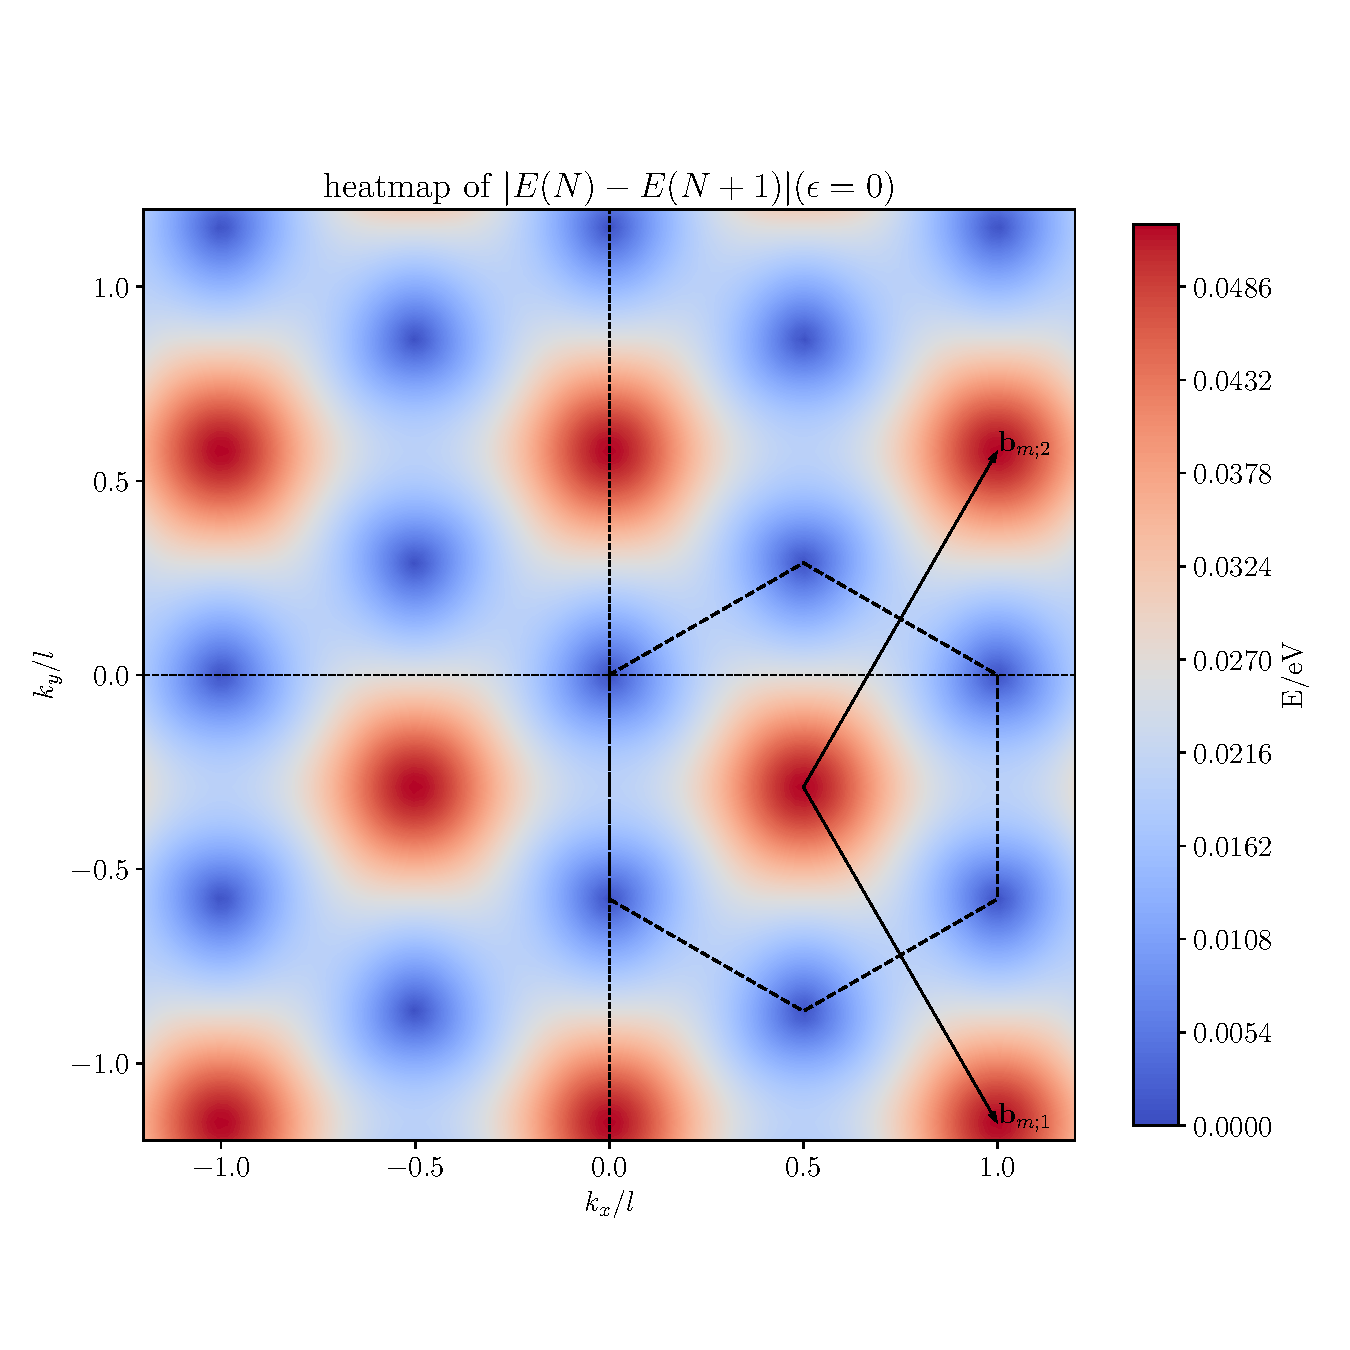
\includegraphics[width=0.4\linewidth]{pic/strain/nostrain_new.pdf} 
    \caption{Band gap \(E(N+1) - E(N)\) without strain.}
\end{figure*}

where the unit of \((kx,ky)\) axis is \(l = \frac{8 \pi \sin(\te/2)}{\sqrt{3} a}\) which is the magnitude of the Moiré reciprocal lattice vector.


\begin{figure}[h!]
    \centering
    \subfigure[gap]{
        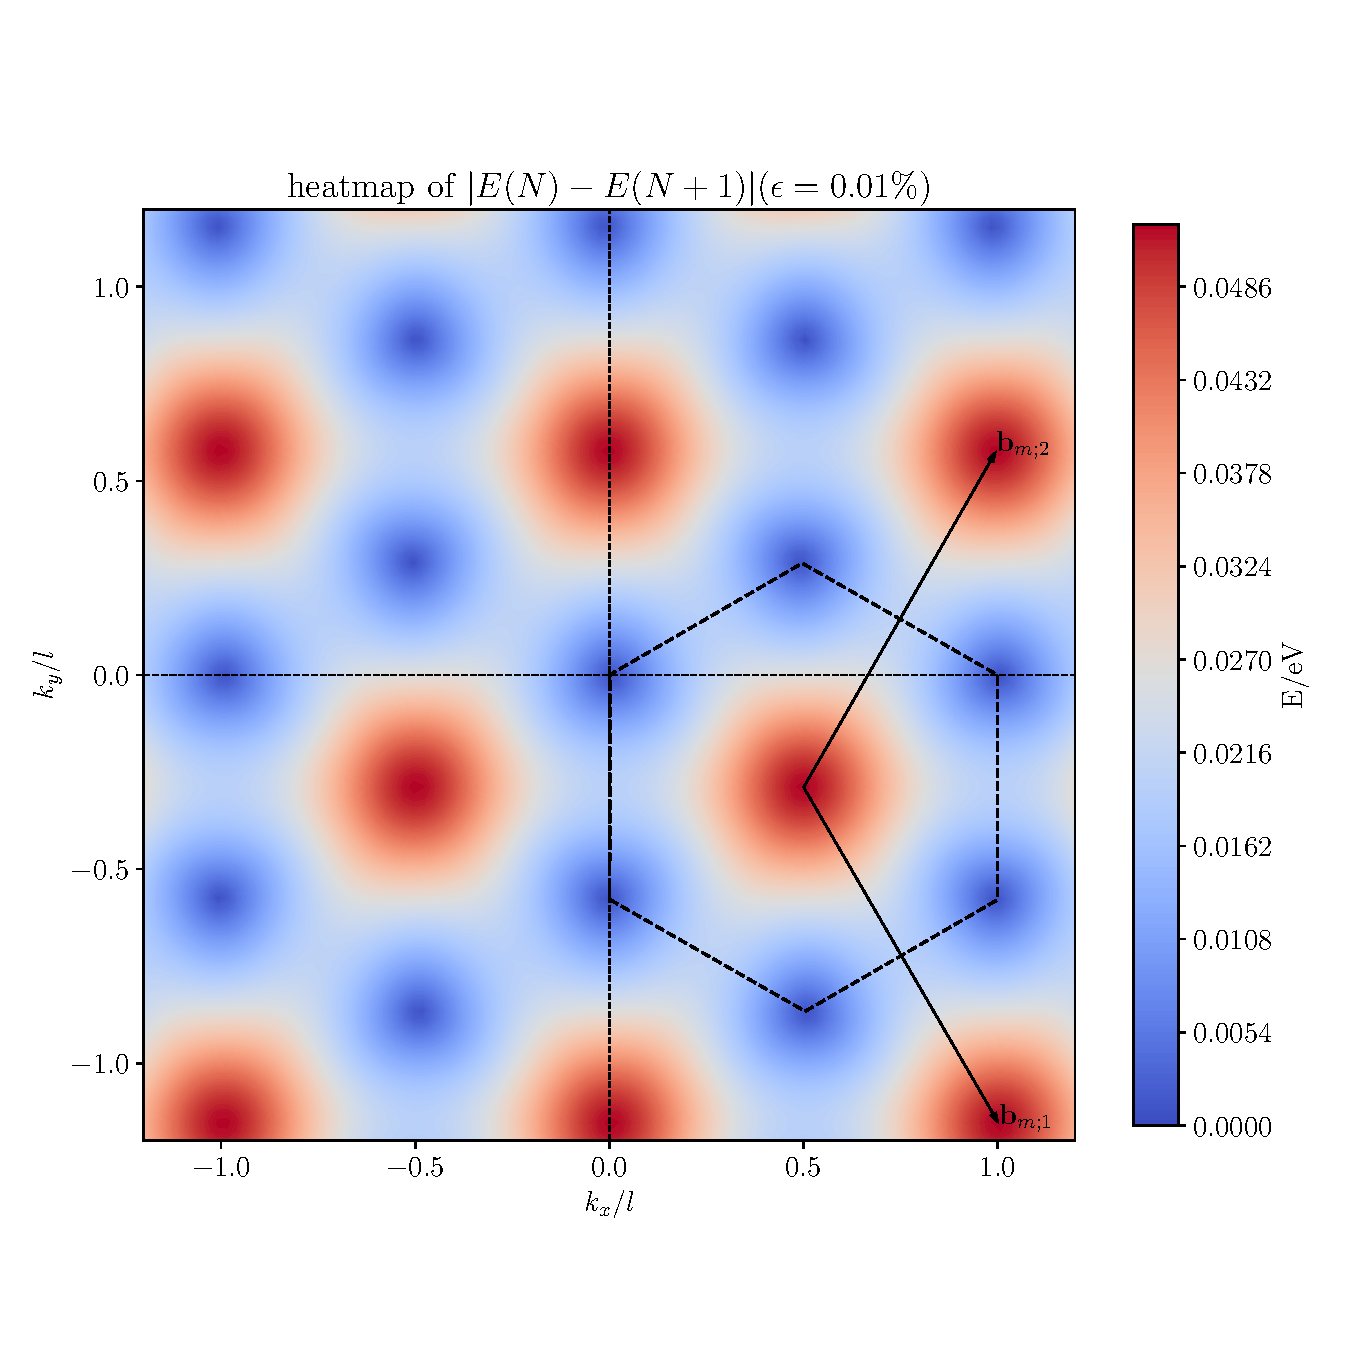
\includegraphics[width=0.3\textwidth]{pic/strain_te_10/gap_0_0001.pdf}
    }
    \subfigure[EN]{
        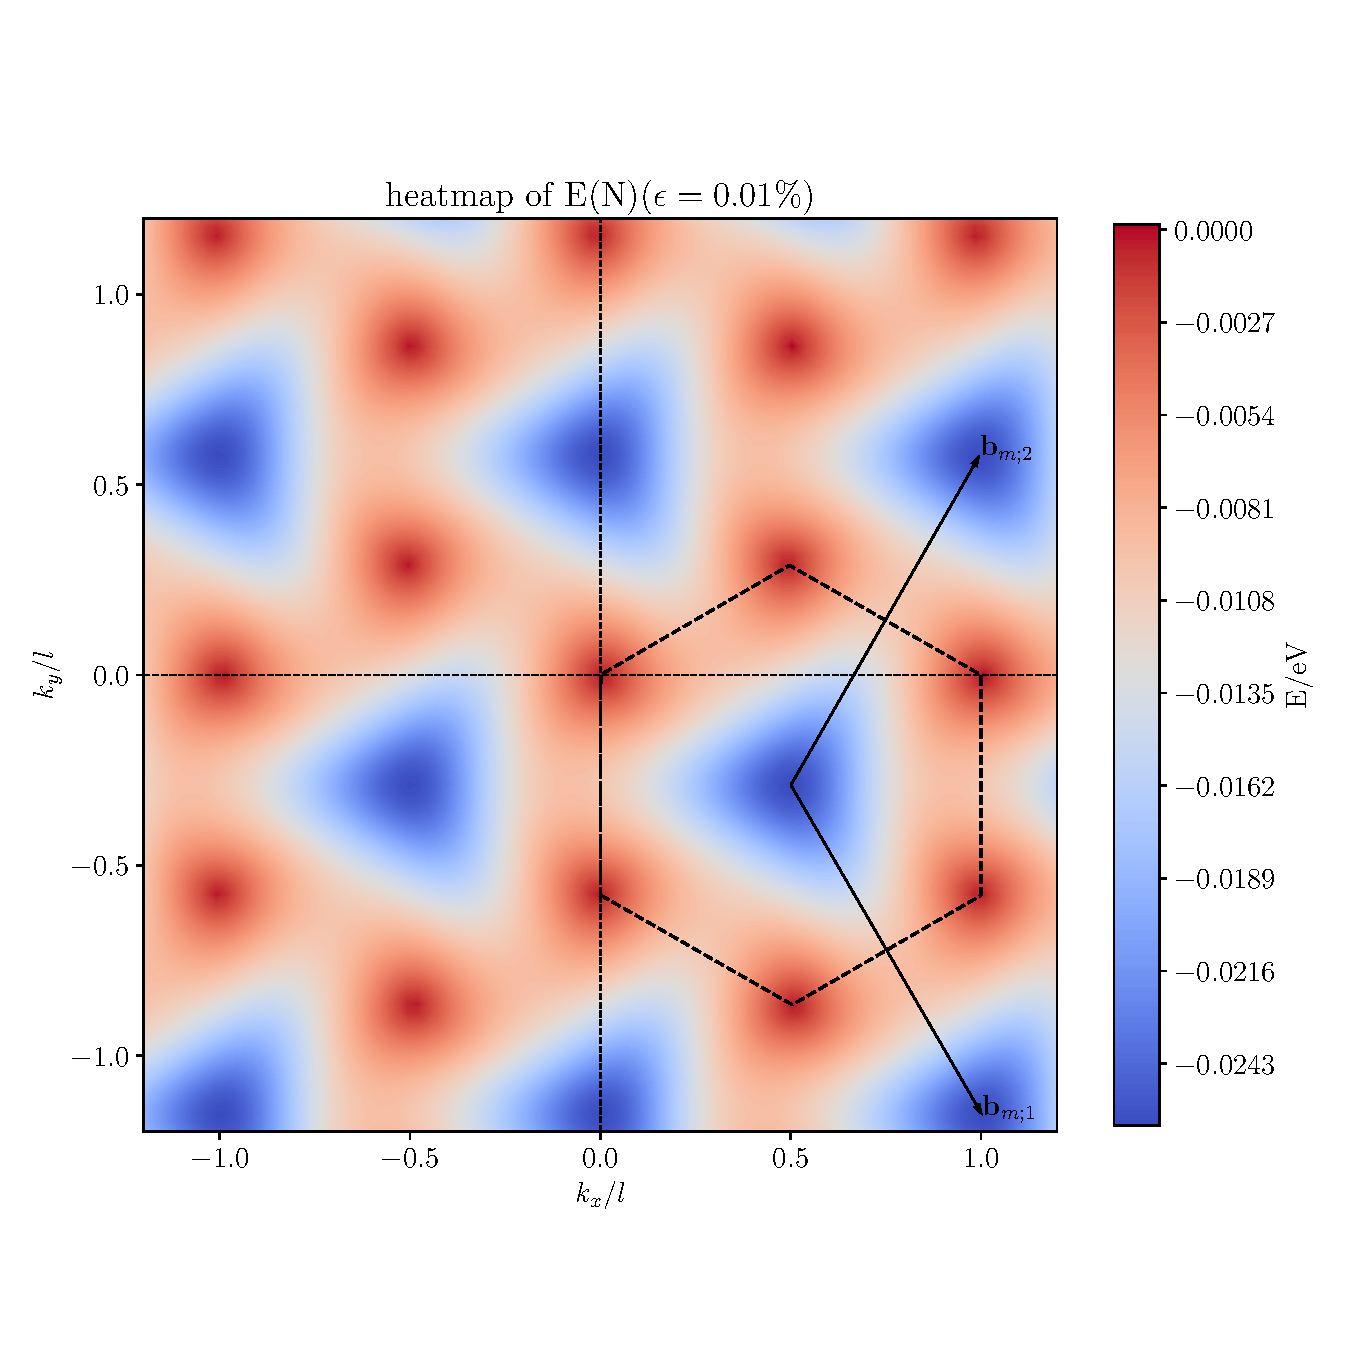
\includegraphics[width=0.3\textwidth]{pic/strain_te_10/EN_0_0001.pdf}
    }
	\subfigure[EN1]{
		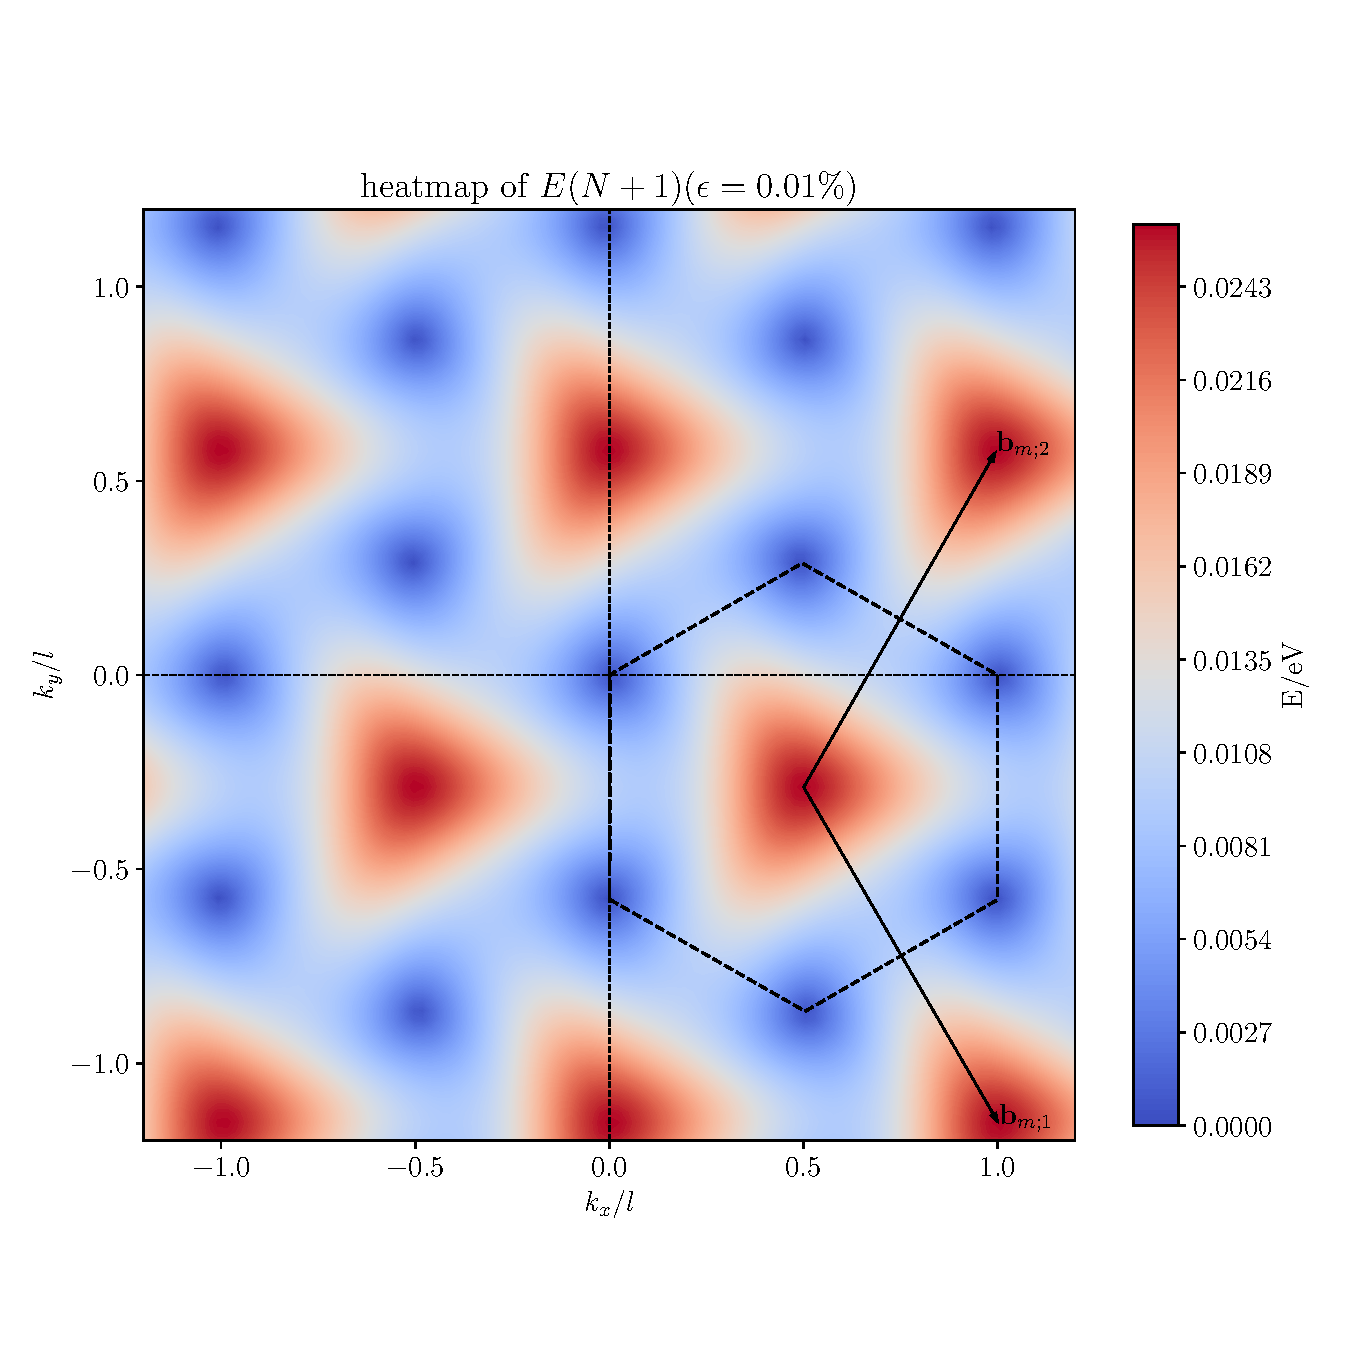
\includegraphics[width=0.3\textwidth]{pic/strain_te_10/EN1_0_0001.pdf}
	}
    \caption{\(\epsilon = 0.01\%, \phi = 10^{\circ}\)}
\end{figure}


\begin{figure}[h!]
    \centering
    \subfigure[$\epsilon = 0.05\%$]{
        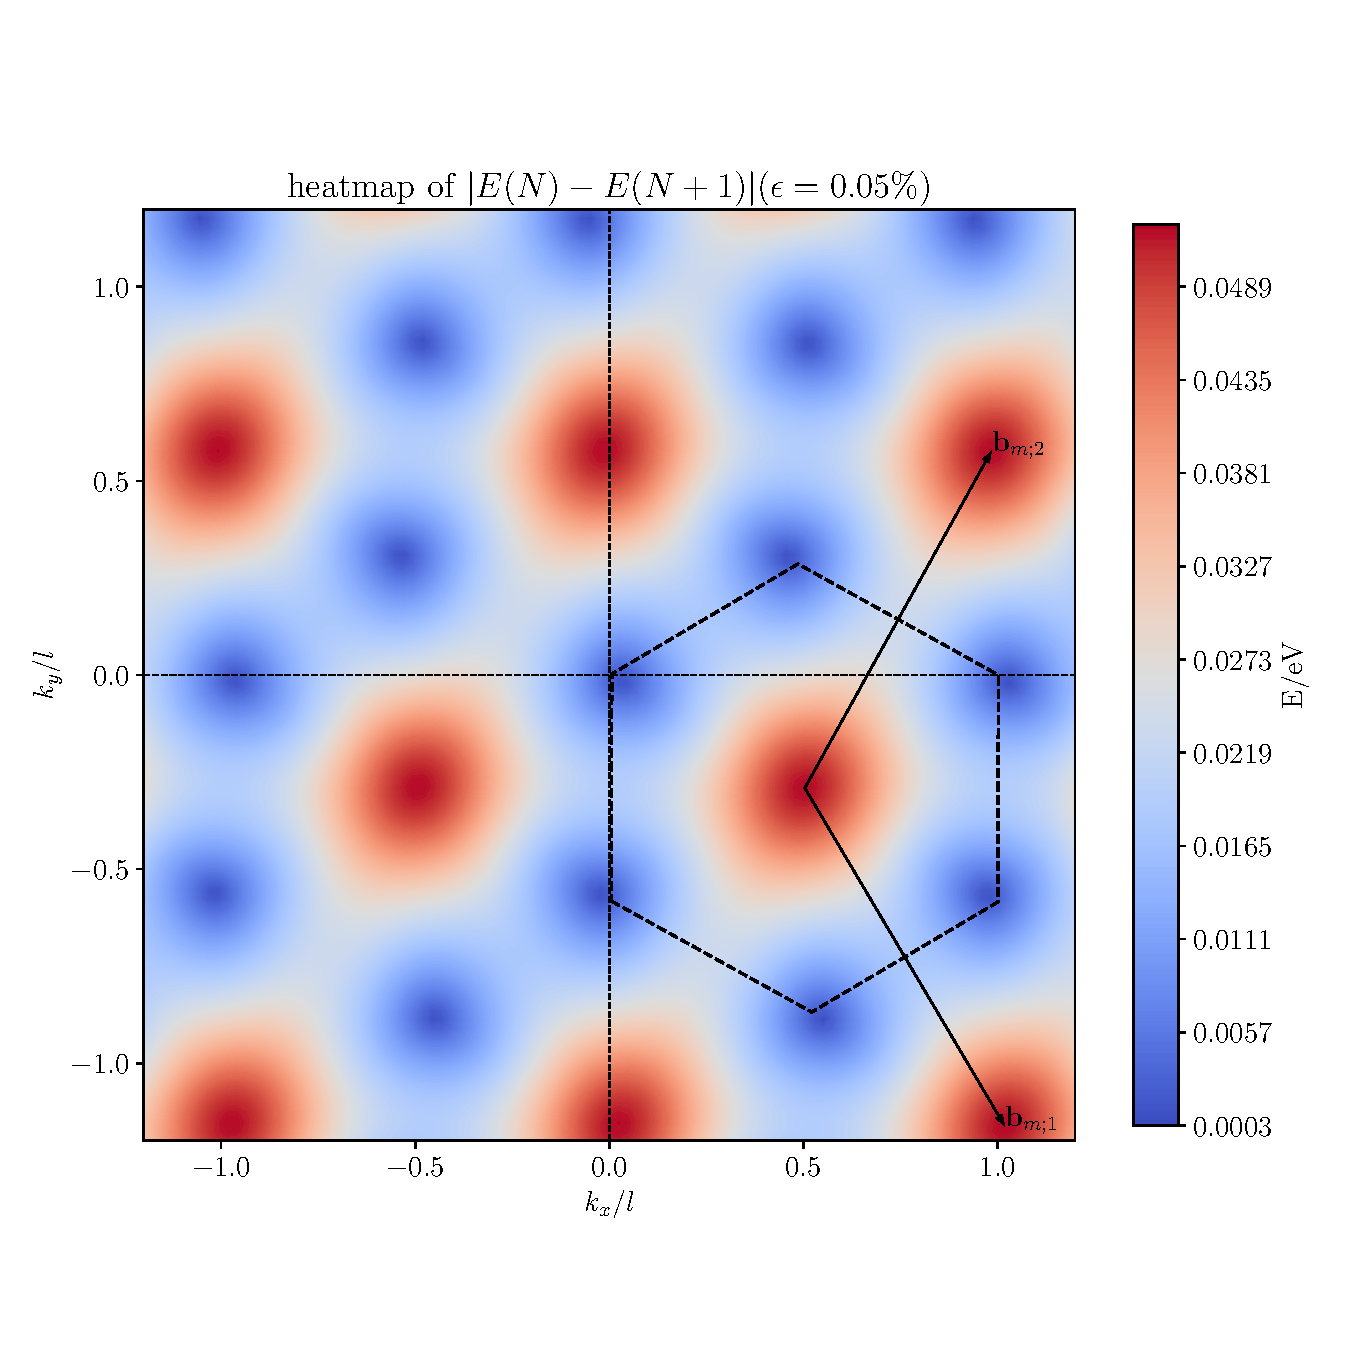
\includegraphics[width=0.3\textwidth]{pic/strain_te_10/gap_0_0005.pdf}
    }
    \subfigure[$\epsilon = 0.1\%$]{
        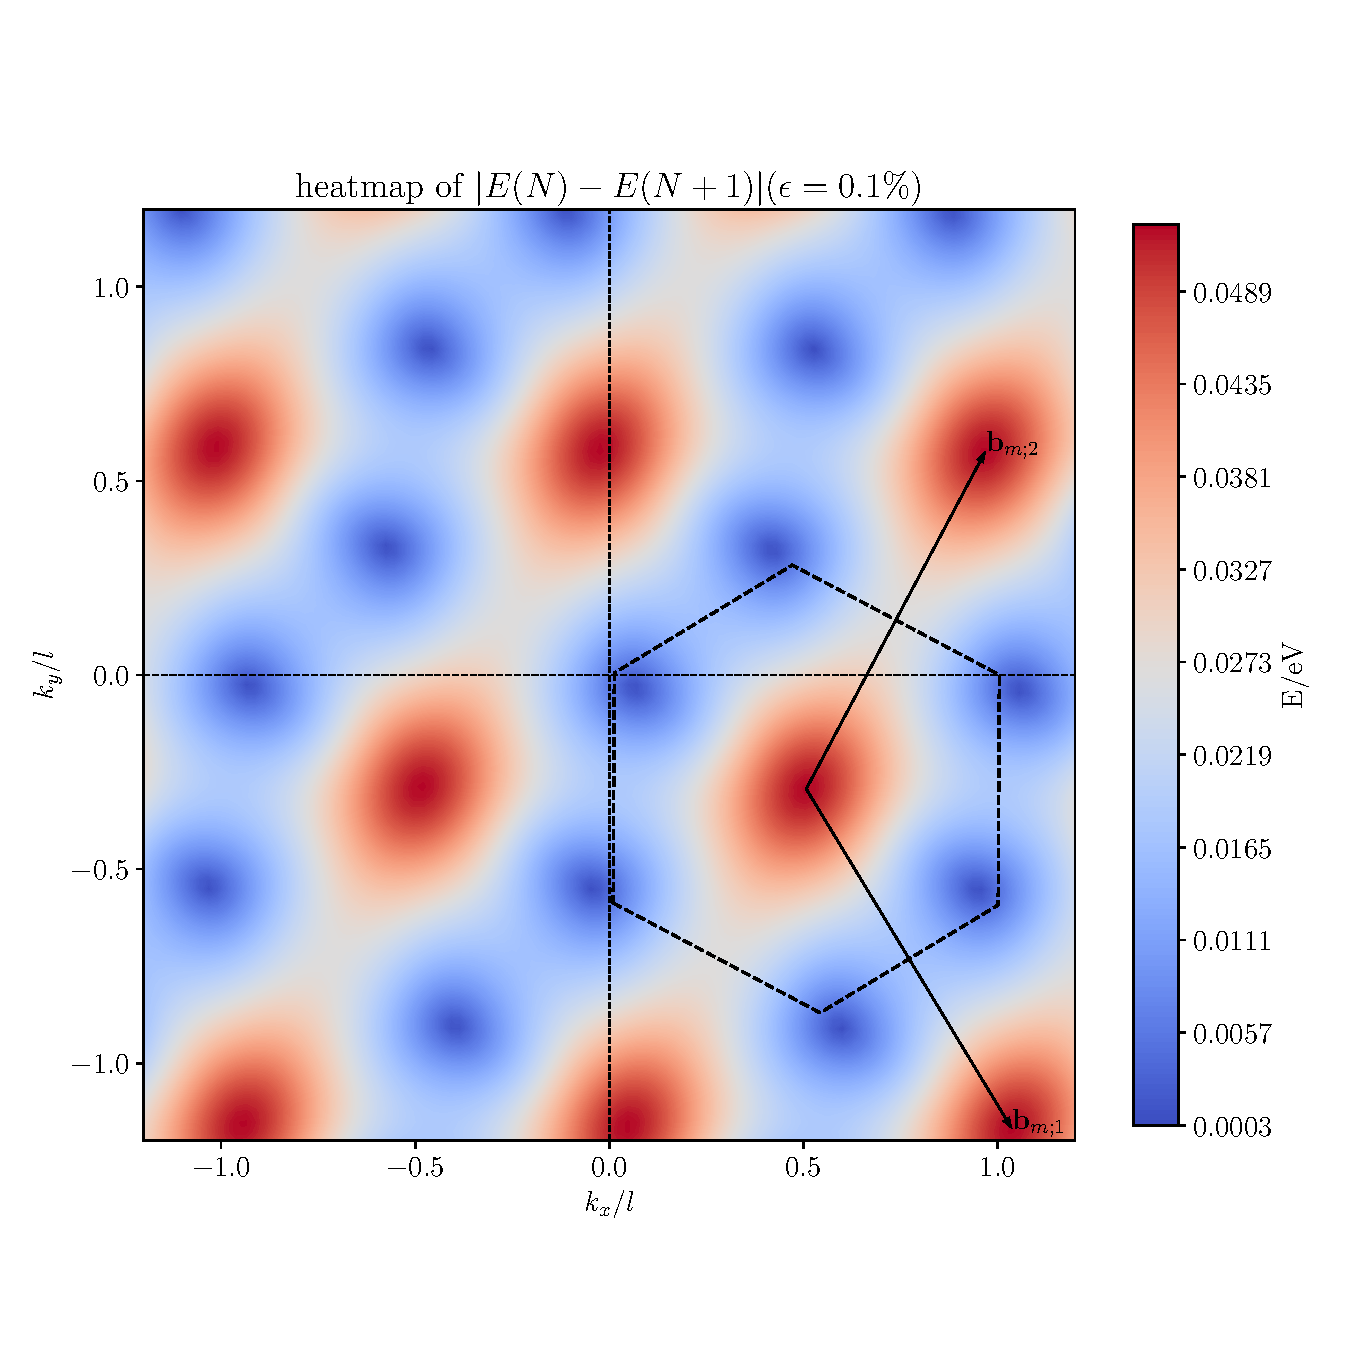
\includegraphics[width=0.3\textwidth]{pic/strain_te_10/gap_0_001.pdf}
    }
	\subfigure[$\epsilon = 0.2\%$]{
		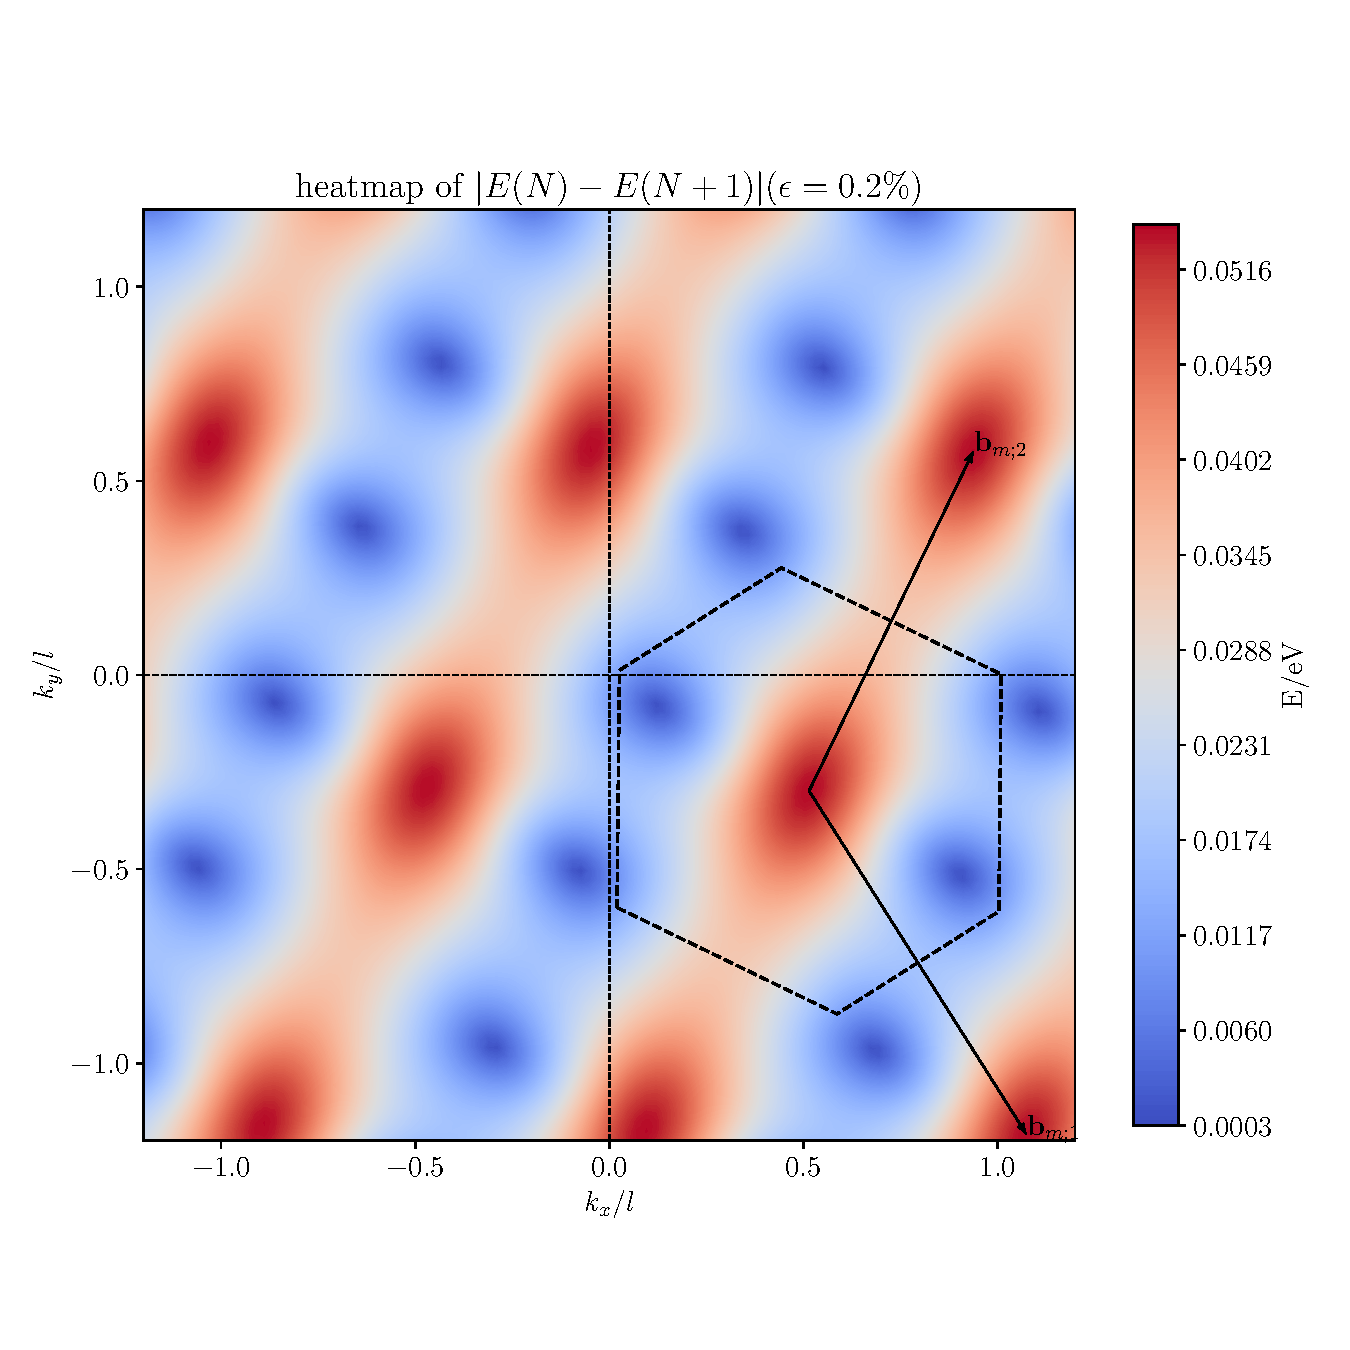
\includegraphics[width=0.3\textwidth]{pic/strain_te_10/gap_0_002.pdf}
	}
    \caption{gap with different strain magnitudes \(\epsilon,\,  \phi = 10^{\circ}\)}
\end{figure}

After scanning the band gap for different strain magnitudes. we searched for the shifted Dirac points and get the energy of shifted Dirac poins, which is 
\begin{figure}[h!]
	\centering
	\subfigure[$\phi = 10^{\circ}$]{
		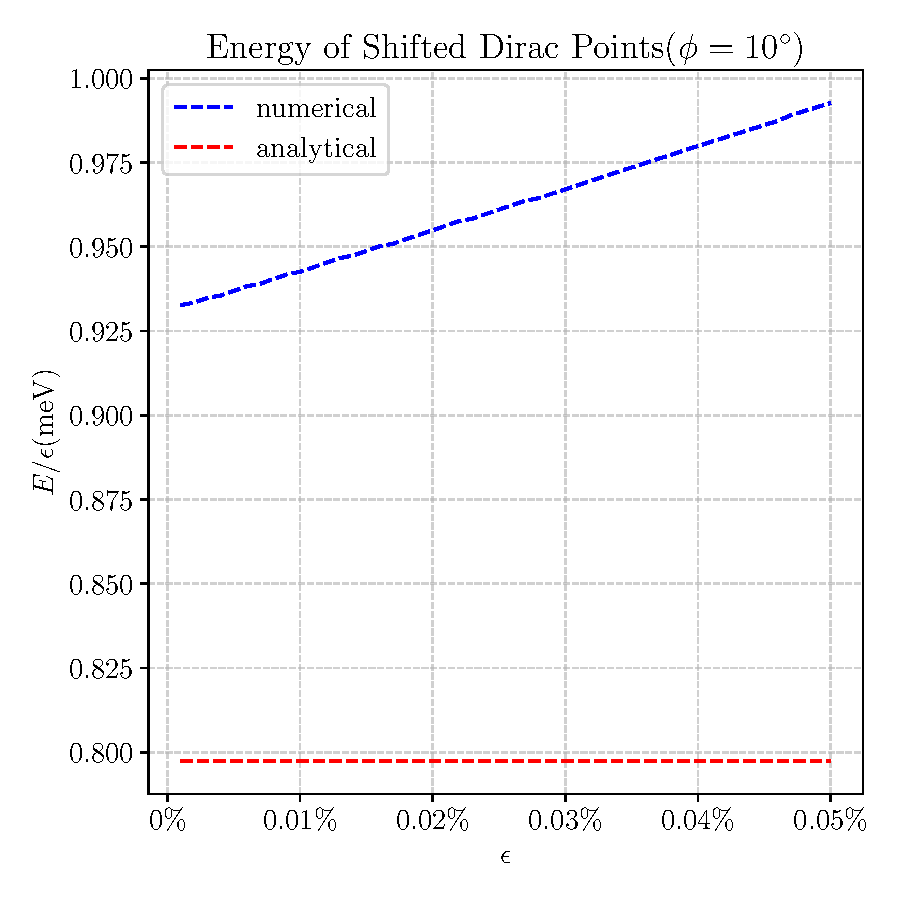
\includegraphics[width=0.35\linewidth]{pic/comp/comp_phi_10_k.pdf} 
	}
	\subfigure[$E-\epsilon$ with different \(\phi\)]{
		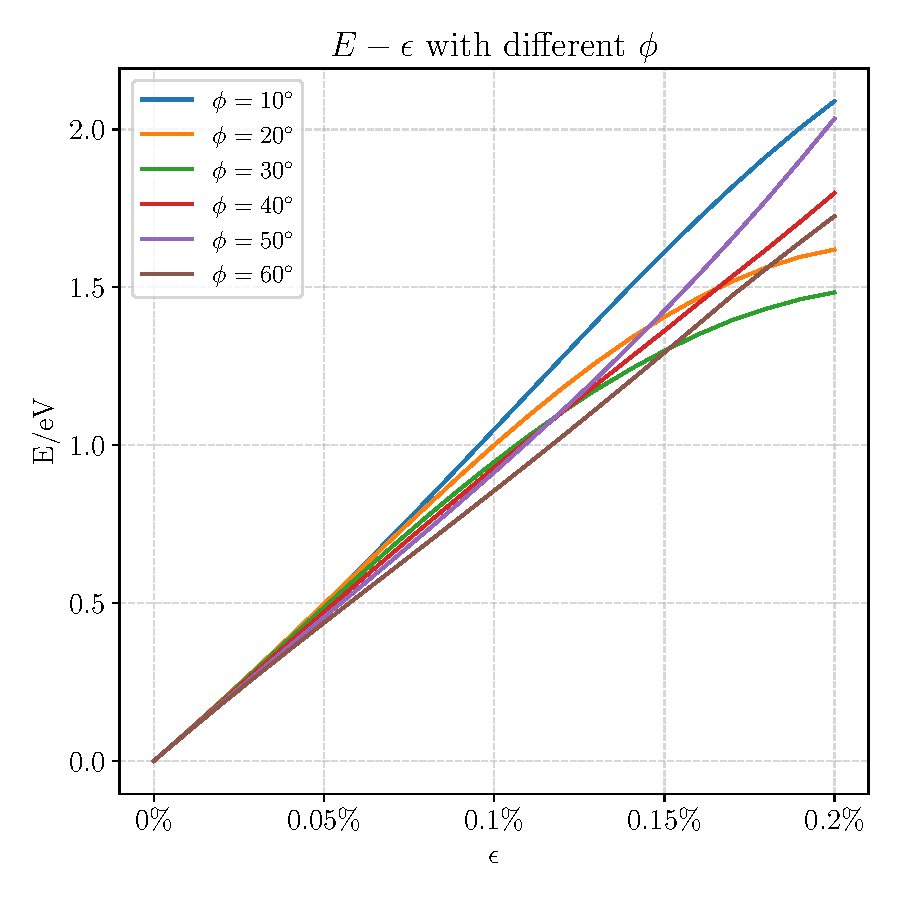
\includegraphics[width=0.35\linewidth]{pic/strain/phi.pdf} 
	}
	\caption{Energy of shifted Dirac points with different \(\phi\).}
\end{figure}


We also compare the analytical and numerical results of different strain directions
\begin{figure}[h!]
	\centering
	\subfigure[$\phi = 20^{\circ}$]{
        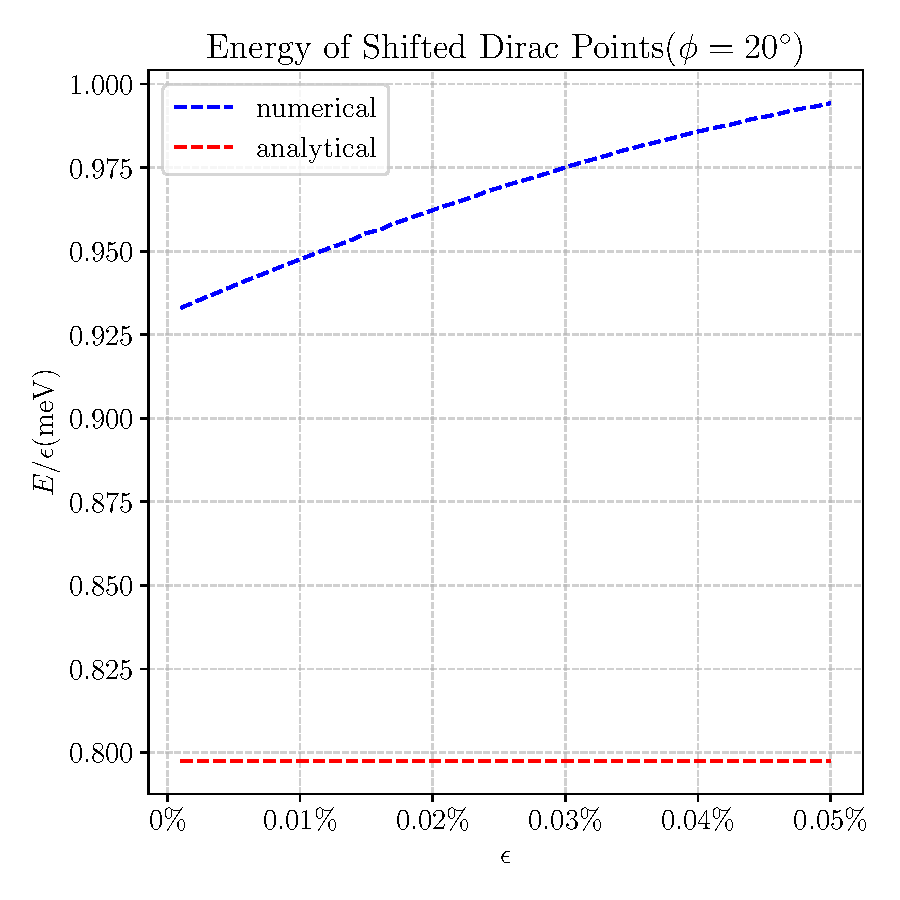
\includegraphics[width=0.35\textwidth]{pic/comp/comp_phi_20_k.pdf}
    }
    \subfigure[$\phi = 40^{\circ}$]{
        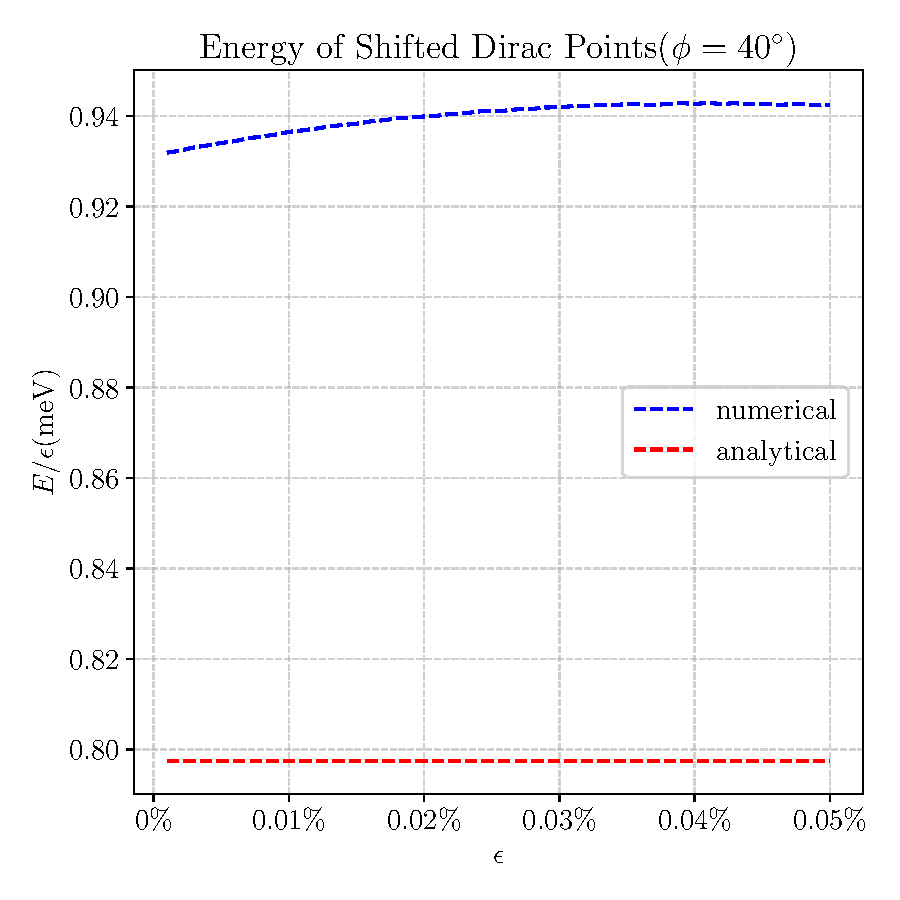
\includegraphics[width=0.35\textwidth]{pic/comp/comp_phi_40_k.pdf}
    }
	\subfigure[$\phi = 50^{\circ}$]{
		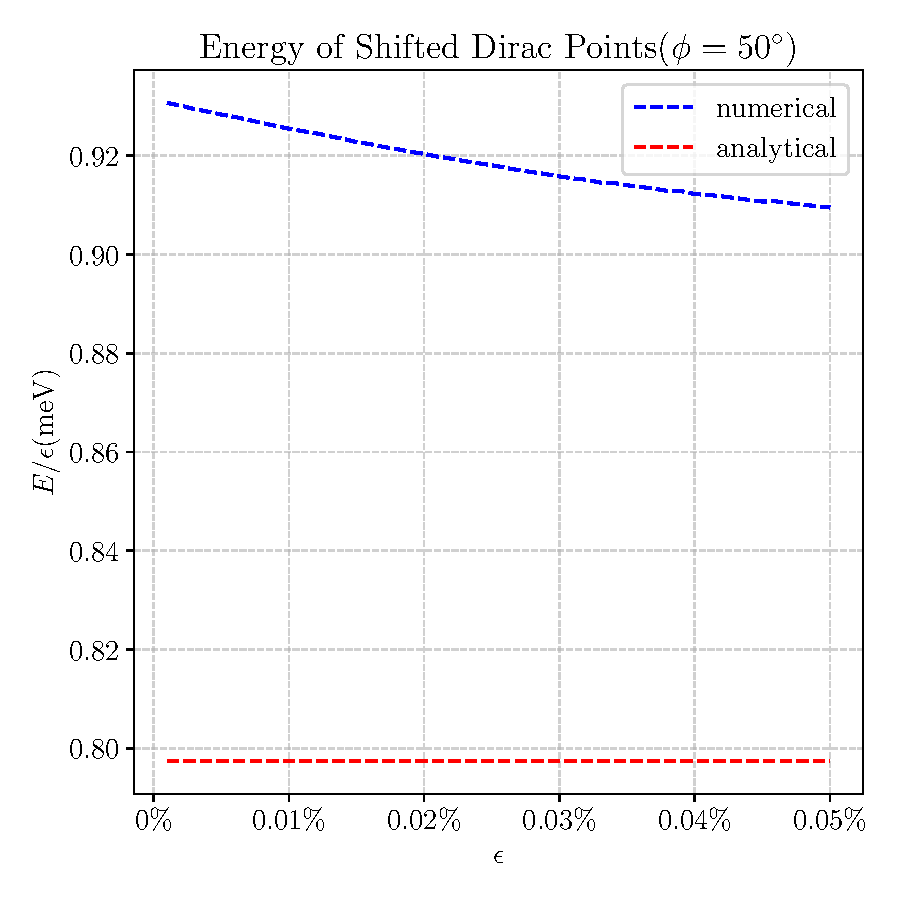
\includegraphics[width=0.35\textwidth]{pic/comp/comp_phi_50_k.pdf}
	}
		\subfigure[$\phi = 60^{\circ}$]{
		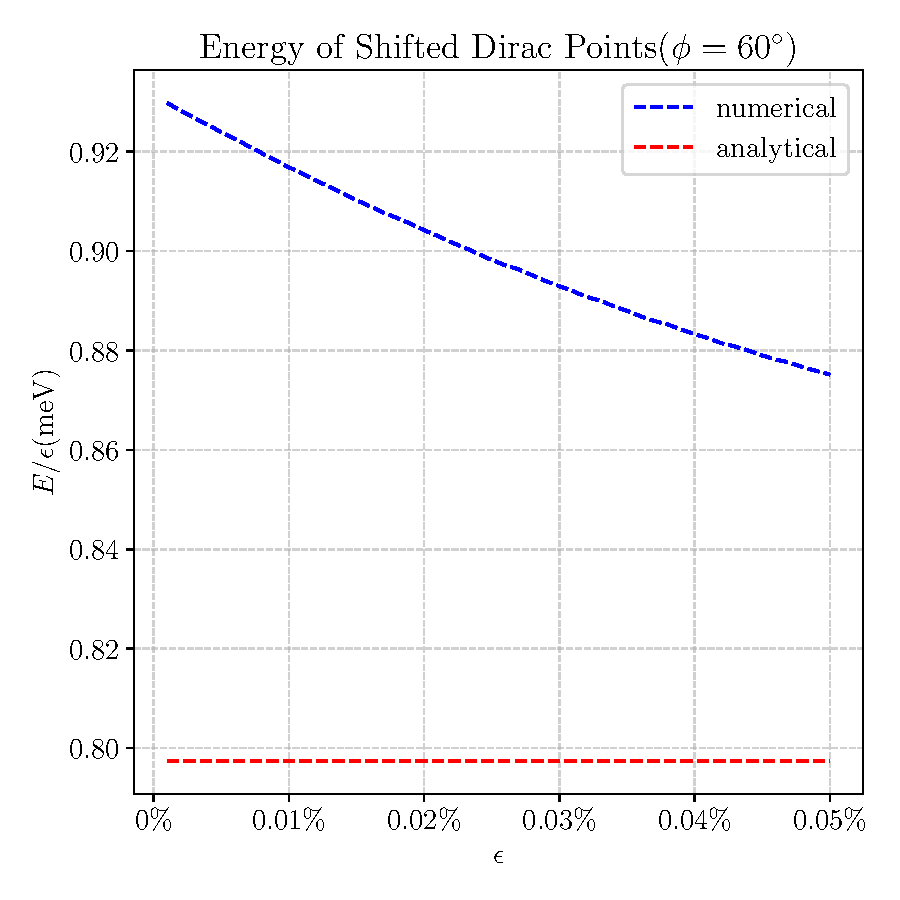
\includegraphics[width=0.35\textwidth]{pic/comp/comp_phi_60_k.pdf}
	}
    \caption{$E$ with different strain directions \( \phi \). where the red line represents the analytical result. The blue line next to the red line is the numerical energy of the shifted Dirac points in top layer and the bottom blue line represents the energy of shifted Dirac points in the bottom layer. \textcolor{red}{(the unit is \(\mr{eV}\))}}
\end{figure}

\begin{itemize}
	\item other results
\end{itemize}
\begin{figure}[h!]
	\centering
	\subfigure[\(\phi = 0^\circ\)]{
		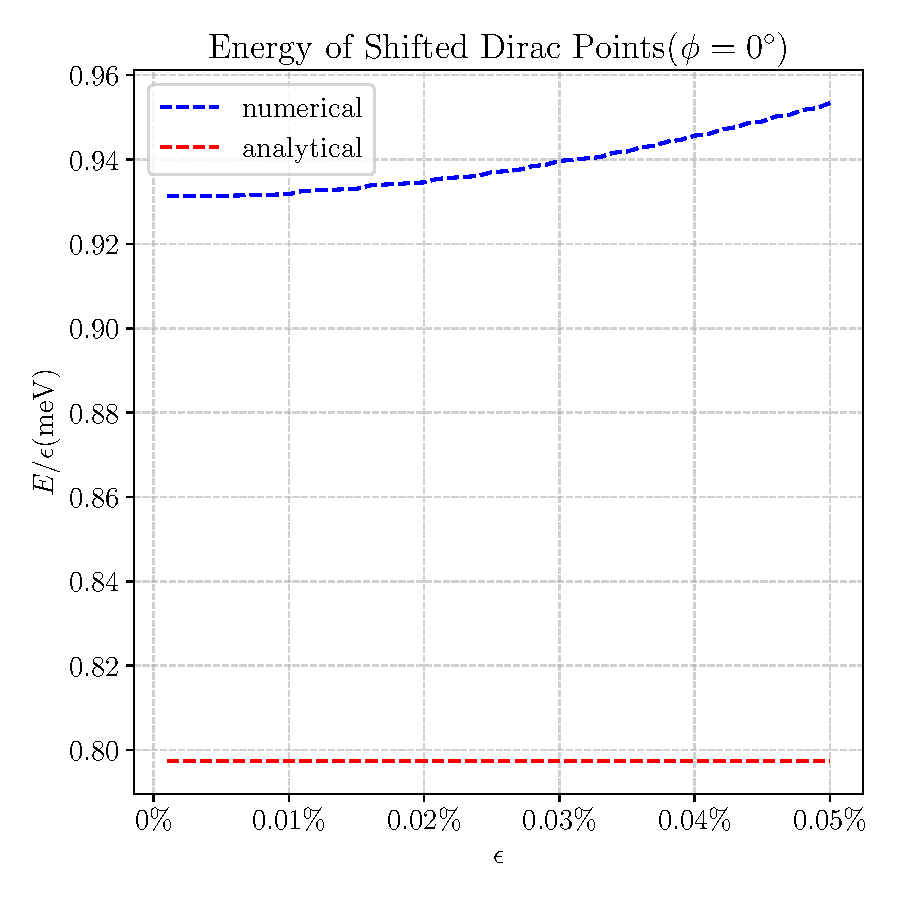
\includegraphics[width=0.3\linewidth]{pic/comp/comp_phi_0.pdf}
	}
	\subfigure[\(\phi = 10^\circ\), \(20 \times 20\) Hamiltonian ]{
		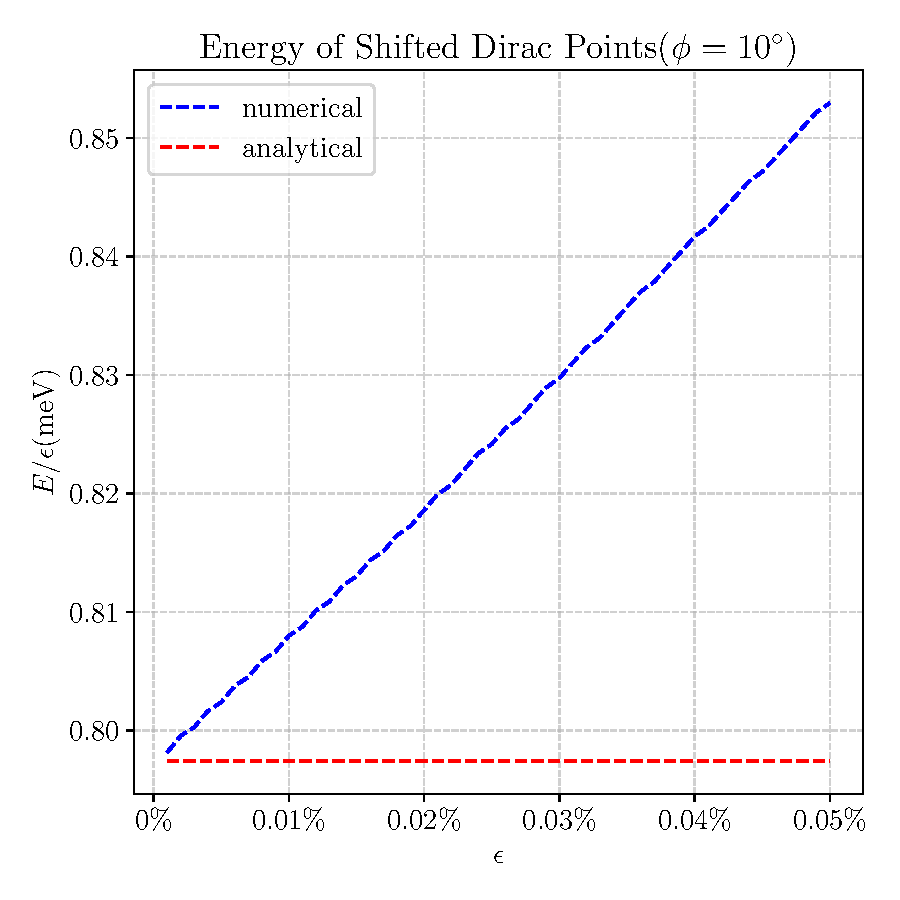
\includegraphics[width=0.3\linewidth]{pic/comp/comp_phi_10_k_20BY20.pdf}
	}
    \caption{Energy of shifted Dirac points with different \(\epsilon\)}
\end{figure}

\begin{itemize}
	\item Symmetry analysis
\end{itemize}
\textcolor{red}{Due to the different convention with Prof. Kang, we change the sign of the \(y\) component of the pseudovector \(\bm{A}\) which is \(A_{y} \rightarrow -A_{y}\),} which is \(A = \begin{pmatrix}
	\p{\epsilon_{1} - \epsilon_{2}} \cos{2\phi} & \p{\epsilon_1 - \epsilon_2} \sin{2\phi}
\end{pmatrix}\)

\begin{figure}[h!]
	\centering
	\subfigure[different \(\epsilon\)]{
		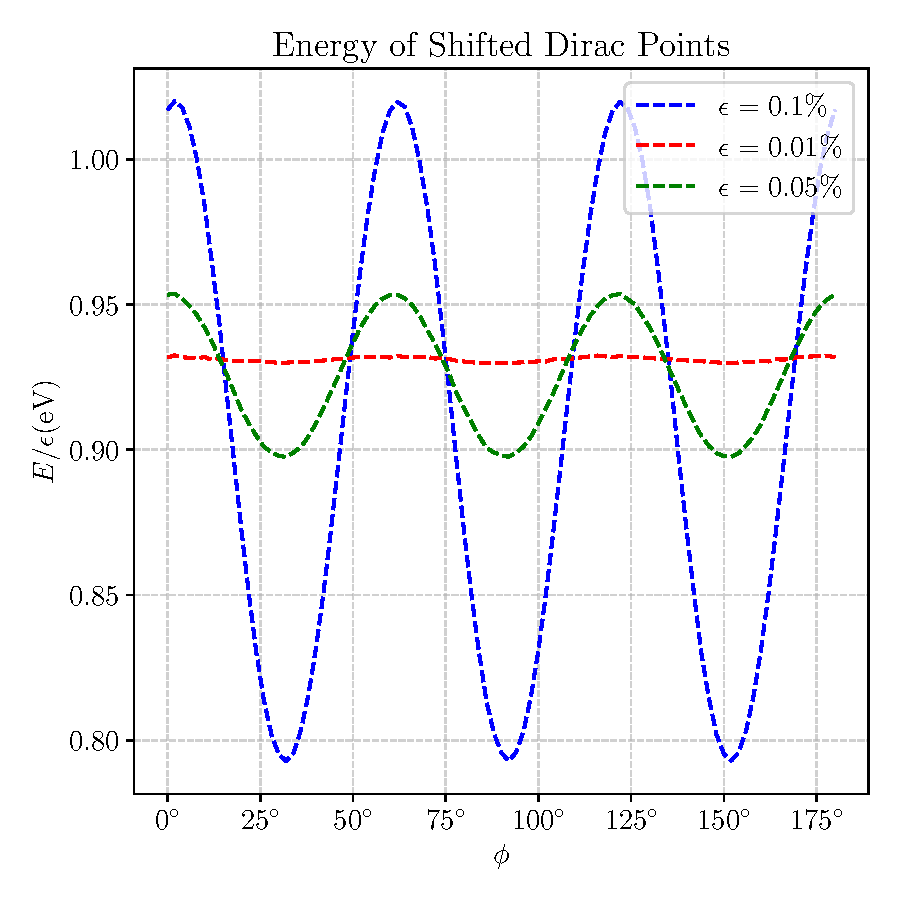
\includegraphics[width=0.3\linewidth]{pic/further/comp_epsilon.pdf}
	}
	\subfigure[different \(\phi\)]{
	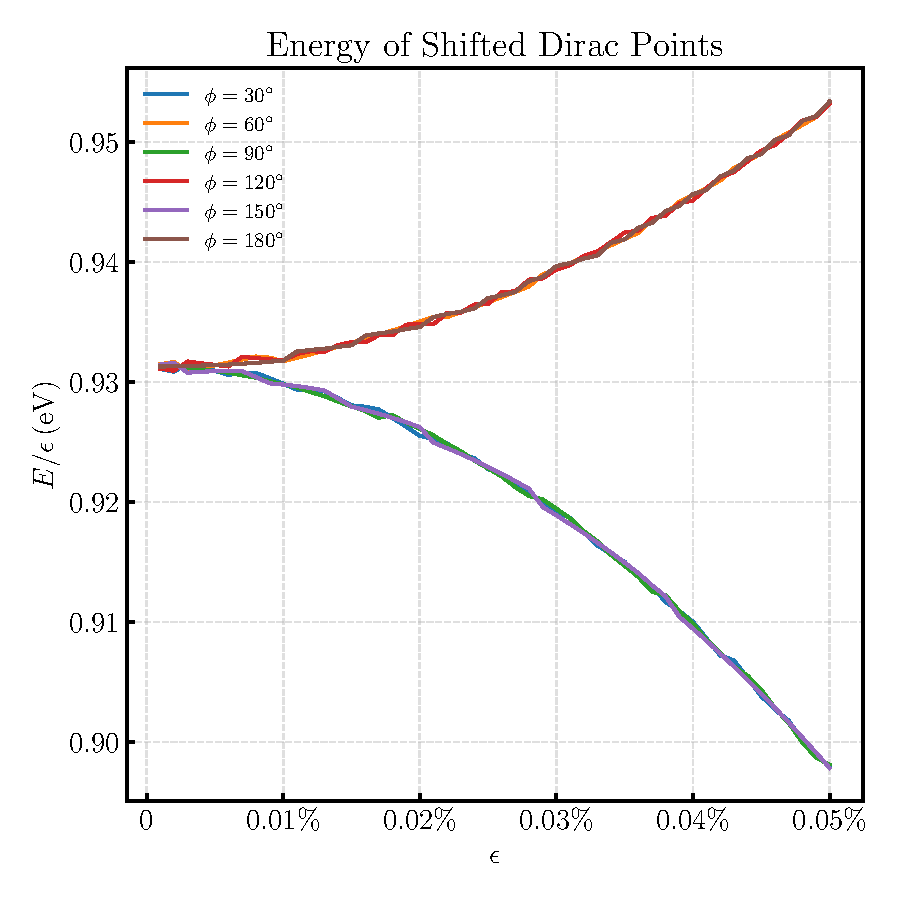
\includegraphics[width=0.3\linewidth]{pic/further/comp_phi.pdf}
	}
    \caption{Energy of shifted Dirac points}
\end{figure}

The energy of the Dirac points exhibits a periodicity of \(\pi/3\) with respect to the strain direction \(\phi\). Given the \(C_{3z}\) symmetry of the pristine BM model(period \(2 \pi/3\)) and the \(C_{2z}\) symmetry of the strain tensor ( \(\mathcal{S} \p{\epsilon, \phi} = \mathcal{S} \p{\epsilon, \phi + \pi} \)), leads to the modulation period of \(\pi/3\), which corresponds to the greatest common divisor of these two rotational periods. So if we expand the energy of Dirac points(top layer), we only have these terms:
\begin{align}
	E^{t}_{\mr{DP}}  = A \epsilon + B \epsilon^{2} + \epsilon^3 \p{C_1 + C_{2} \cos{6 \phi} + C_{3} \sin{6 \phi}} + O\p{\epsilon^{4}, 8 \phi},
\end{align}
With particle-hole symmetry \(\mathcal{P} H\p{\bm{k}} \mathcal{P}^{-1} = - H \p{ - \bm{k}}\) which means we map the Dirac points to the other layer. So the energy of Dirac points in the bottom layer is 
\begin{align}
	E^{b}_{\mr{DP}}  = - A \epsilon - B \epsilon^2 - \epsilon^3 \p{C_{1} + C_{2} \cos{6 \phi} + C_{3} \sin{6 \phi}} + O\p{\epsilon^{4}, 8 \phi}.
\end{align}

Also we can exchange the layer index by the \(C_{2x}\) symmetry. However if we need to satisfy the \(C_{2x}\) symmetry under heterostrain, the strain should be transformed as \(\p{\epsilon, \phi} \rightarrow \p{-\epsilon, -\phi}\). Thus the energy of Dirac points changes into 
\begin{align}
	E^{b}_{DP} = - A \epsilon + B \epsilon^2 - \epsilon^3 \p{C_{1} + C_{2} \cos{6 \phi} - C_{3} \sin{6 \phi}} + O\p{\epsilon^{4}, 8 \phi},
\end{align}
So \(B = C_{3} = 0\). We can rewrite the energy of Dirac points as
\begin{align}
	\boxed{
		\frac{E_{DP}}{\epsilon} = A + \epsilon^{2} \p{C_{1} + C_{2} \cos{6 \phi}}.
	}
\end{align}
By fitting the data, we can get \(C_2 \gg C_{1}\).


\section{van Hove singularity and DOS}
\subsection{Definition of DOS}
In solid state physics, the DOS \(D\p{E}\) describes the number of electronic states available at each energy level for electrons to occupy. For every single \(\bm{k}\) it contributes two states (spin up and down), so the DOS can be expressed as how many \(\bm{k}\) points exist in the same energy \(\mr{d} E\). In two-dimensional systems, the DOS is given by
\begin{align}
	D\p{E} = \sum_{j} \frac{2}{\p{2 \pi}^{2}} \oint_{E\p{\bm{k} = E}} \frac{\mr{d} \bm{l}}{ \bv{\nabla_{\bm{k}} E_{j} \p{\bm{k}}}},
\end{align}
where the \(\bv{\nabla_{\bm{k}} E_{j} \p{\bm{k}}}\) is the gradient of the energy with respect to the momentum \(\bm{k}\) in the \(j\)-th band which is also the group velocity of electrons.
\begin{align}
	\bm{v} = \frac{\mr{d} \bm{r}}{\mr{d} t} = \frac{1}{\hbar} \nabla_{\bm{k}} E_{j} \p{\bm{k}}
\end{align}

We can use the Dirac delta function to rewrite the DOS as
\begin{align}
	D\p{E} =  \sum_{j} \frac{2}{\p{2 \pi}^{2}} \iint_{BZ} \delta \p{E - E\p{\bm{k}}} \mr{d}^{2} \bm{k}.
\end{align} 
Numerically, we can calculate the DOS by using the Gaussian broadening method. The delta function can be approximated as
\begin{align}
	\delta \p{E - E\p{\bm{k}}} \approx \frac{1}{\sqrt{2 \pi} \sigma} \exp{ \bb{-\frac{\p{E - E\p{\bm{k}}}^{2}}{2 \sigma^{2}}}},
\end{align}
where \(\sigma\) is the broadening parameter which determines the width of the Gaussian function. Thus the DOS can be calculated as
\begin{align}
	D\p{E} \approx \frac{1}{N_k} \sum_{k = 1}^{N_k}\frac{1}{\sqrt{2 \pi} \sigma} \exp{ \bb{-\frac{\p{E - E\p{\bm{k}}}^{2}}{2 \sigma^{2}}}},
\end{align}
where \(N_k\) is the total number of k-points sampled in the moiré Brillouin zone.

Here is another way to calcaulate the DOS numerically which called \textit{triangle method(2D version of tetrahedron method)}. The basic idea is to replace the Gaussian broadening with an analytic evaluation of the BZ integral under the assumption that the band energy is linear on each small triangle of a triangulated Brillouin zone. Firstly, we can construct a uniform mesh in the first (moire) Brillouin zone like 
\begin{align}
	\bm{k}_{i,j} = \frac{i}{N_{x}} \bm{b}^{m}_{1} + \frac{j}{N_{y}} \bm{b}^{m}_{2},
\end{align}
and for each square mesh cell, we can divide it into two triangles by the main diagonal: triangle A with vertices \(\p{i,j},\p{i+1, j}, \p{i+1, j+1}\) and triangle B with vertices \(\p{i,j},\p{i, j+1}, \p{i+1, j+1}\). Then we can linearly interpolate the energy within each triangle. For triangle A, the energy at any point \(\bm{k}\) inside the triangle can be expressed as
\begin{align}
	E\p{\bm{k}} = E_0 + \nabla_{\bm{k}}E \p{\bm{k} - \bm{k}_0},
\end{align}
or 
\begin{align}
	E\p{\bm{k}} = a k_x + b k_y + c,
\end{align}
where the energy gradient \(\nabla_{\bm{k}} E\) is constant within the triangle.   

Before we have the definition of DOS which is 
\begin{align}
	D\p{E} = \frac{1}{\p{2 \pi}^2} \int_{\mr{BZ}} \delta \p{E - E\p{\bm{k}}} \mr{d}^{2} \bm{k}.
\end{align}
We can make a projection from the k-space \(\p{k_x, k_y}\) to energy space \(\p{\nabla E, E}\) or \(\p{s,u}\) with the Jacobian factor \(dk_x dk_{y} = \frac{1}{\bv{\nabla_{\bm{k}} E}} ds du\) and the integral becomes
\begin{align} \label{DOS}
	\begin{split}
		D\p{E}  & =  \frac{1}{\p{2 \pi}^2} \int_{\mr{BZ}} \delta \p{E - E\p{\bm{k}}} \mr{d}^{2} \bm{k}. \\
		& = \int_{s} \int_{u} \delta \p{E - u} \frac{1}{\bv{\nabla_{\bm{k}} E}} ds du \\
		& = \int_{\mr{segment}} \frac{1}{ \bv{\nabla_{\bm{k}} E}} ds \\
		& = \frac{L}{\bv{\nabla_{\bm{k}} E}},
	\end{split}
\end{align} 
where \(L\) is  the isoenergy line segment length within the triangle and \(\bv{\nabla_{\bm{k}} E}\) is the magnitude of the energy gradient within the triangle. If \(E \in  \bb{E_1, E_2}\) we can compute the interpolation parameter 
\begin{align}
	t = \frac{E - E_1}{E_2 - E_1},
\end{align}
and the position of the intersection point on the triangle edges is 
\begin{align}
	\bm{p}_{1} = \bm{k}_1 + t \p{\bm{k}_2 - \bm{k}_1}.
\end{align}
and the length of the isoenergy line segment is
\begin{align}
	L = \bv{\bm{p}_2 - \bm{p}_1}. 
\end{align}

Now we give another expression of \eqref{DOS} which is much simpler. We can define a differential element of area, \(d S\) in k-space. If we move perpendicular to the isoenergy line by a tiny distance \(d l_{\bot}\). Thus, the area swept out is the length of the line times the distance moved 
\begin{align}
	d S = L\p{E} \cdot d l_{\bot},
\end{align}
and the change in energy is the gradient times the distance moved
\begin{align}
	d E = \bv{\nabla_{\bm{k}} E} \cdot d l_{\bot}.
\end{align}
substituting the latter into the former gives
\begin{align}
	d S = L \p{E} \cdot \frac{d E}{\bv{\nabla_{\bm{k}} E}},	
\end{align}
rearranging this expression yields
\begin{align}
	\frac{d S}{d E} = \frac{L \p{E}}{ \bv{\nabla E}} = D \p{E}.
\end{align}
So calculating the length divided by the gradient is mathematically identical to calculating the rate of change of the occupied are with respect to energy.

Now, we just need to calculate the area \(S \p{E}\)  occupied by states wuth energy less than \(E\) within the triangle. If the energies at the three verticres be sorted: \(E_{1} < E_{2} < E_{3}\) and the total area of the flat triangle in k-space is \(S_{\Delta}\). For the initial rise \(E_1 \leq E \leq E_2\) which means the iso-energy line cuts off the single, lowest corner (vertex 1), the area of flat triangle is 
\begin{align}
	S_{\Delta} = \frac{1}{2} L_{12} \cdot L_{13} \sin{\theta},
\end{align}
and the area \(S\p{E}\) is
\begin{align}
	S\p{E} = \frac{1}{2} l_{12} l_{13} \sin{\theta},
\end{align}
where \(l_{12}, l_{13}\) are the lengths of the iso-energy line segments on the edges of the triangle. Using the linear interpolation \(E = E_0 + \bm{v} \cdot \bm{p}\), we have
\begin{align}
	\frac{l_{12} }{L_{12}} = \frac{E - E_1}{E_2 - E_1}, \quad \frac{l_{13} }{L_{13} } = \frac{E - E_1}{E_3 - E_1},
\end{align}
thus the area is
\begin{align}
	S\p{E} = S_{\Delta} \cdot \frac{\p{E - E_1}^{2}}{\p{E_2 - E_1} \p{E_3 - E_1}}.
\end{align}
and the DOS is 
\begin{align}
	D\p{E} = \frac{2 S_{\Delta}}{\p{E_2 - E_1} \p{E_3 - E_1}} \p{E - E_1}.
\end{align}

For the second rise \(E_2 \leq E \leq E_3\), the occupied area \(S \p{E}\) is a complex quadrilateral which the area can be calculated 
\begin{align}
	\begin{split}
		S_{\mr{occupied}} \p{E} &= S_{\Delta} - S_{\mr{unoccupied}} \p{E} \\
		& = S_{\Delta} \bb{1 - \frac{\p{E_{3} - E}^2}{\p{E_{3} - E_{2}} \p{E_{3} - E_{1}}}}
	\end{split}
\end{align}
and the DOS is
\begin{align}
	D\p{E} = \frac{2 S_{\Delta}}{\p{E_{3} - E_{2}} \p{E_{3} - E_{1}}} \p{E_{3} - E}.
\end{align}
When \(E = E_{2}\), both expressions of DOS yield the same result
\begin{align}
	D\p{E_{2}} = \frac{2 S_{\Delta}}{\p{E_{3} - E_{1}}}.
\end{align}

\begin{figure}
	\centering
	\subfigure[]{
		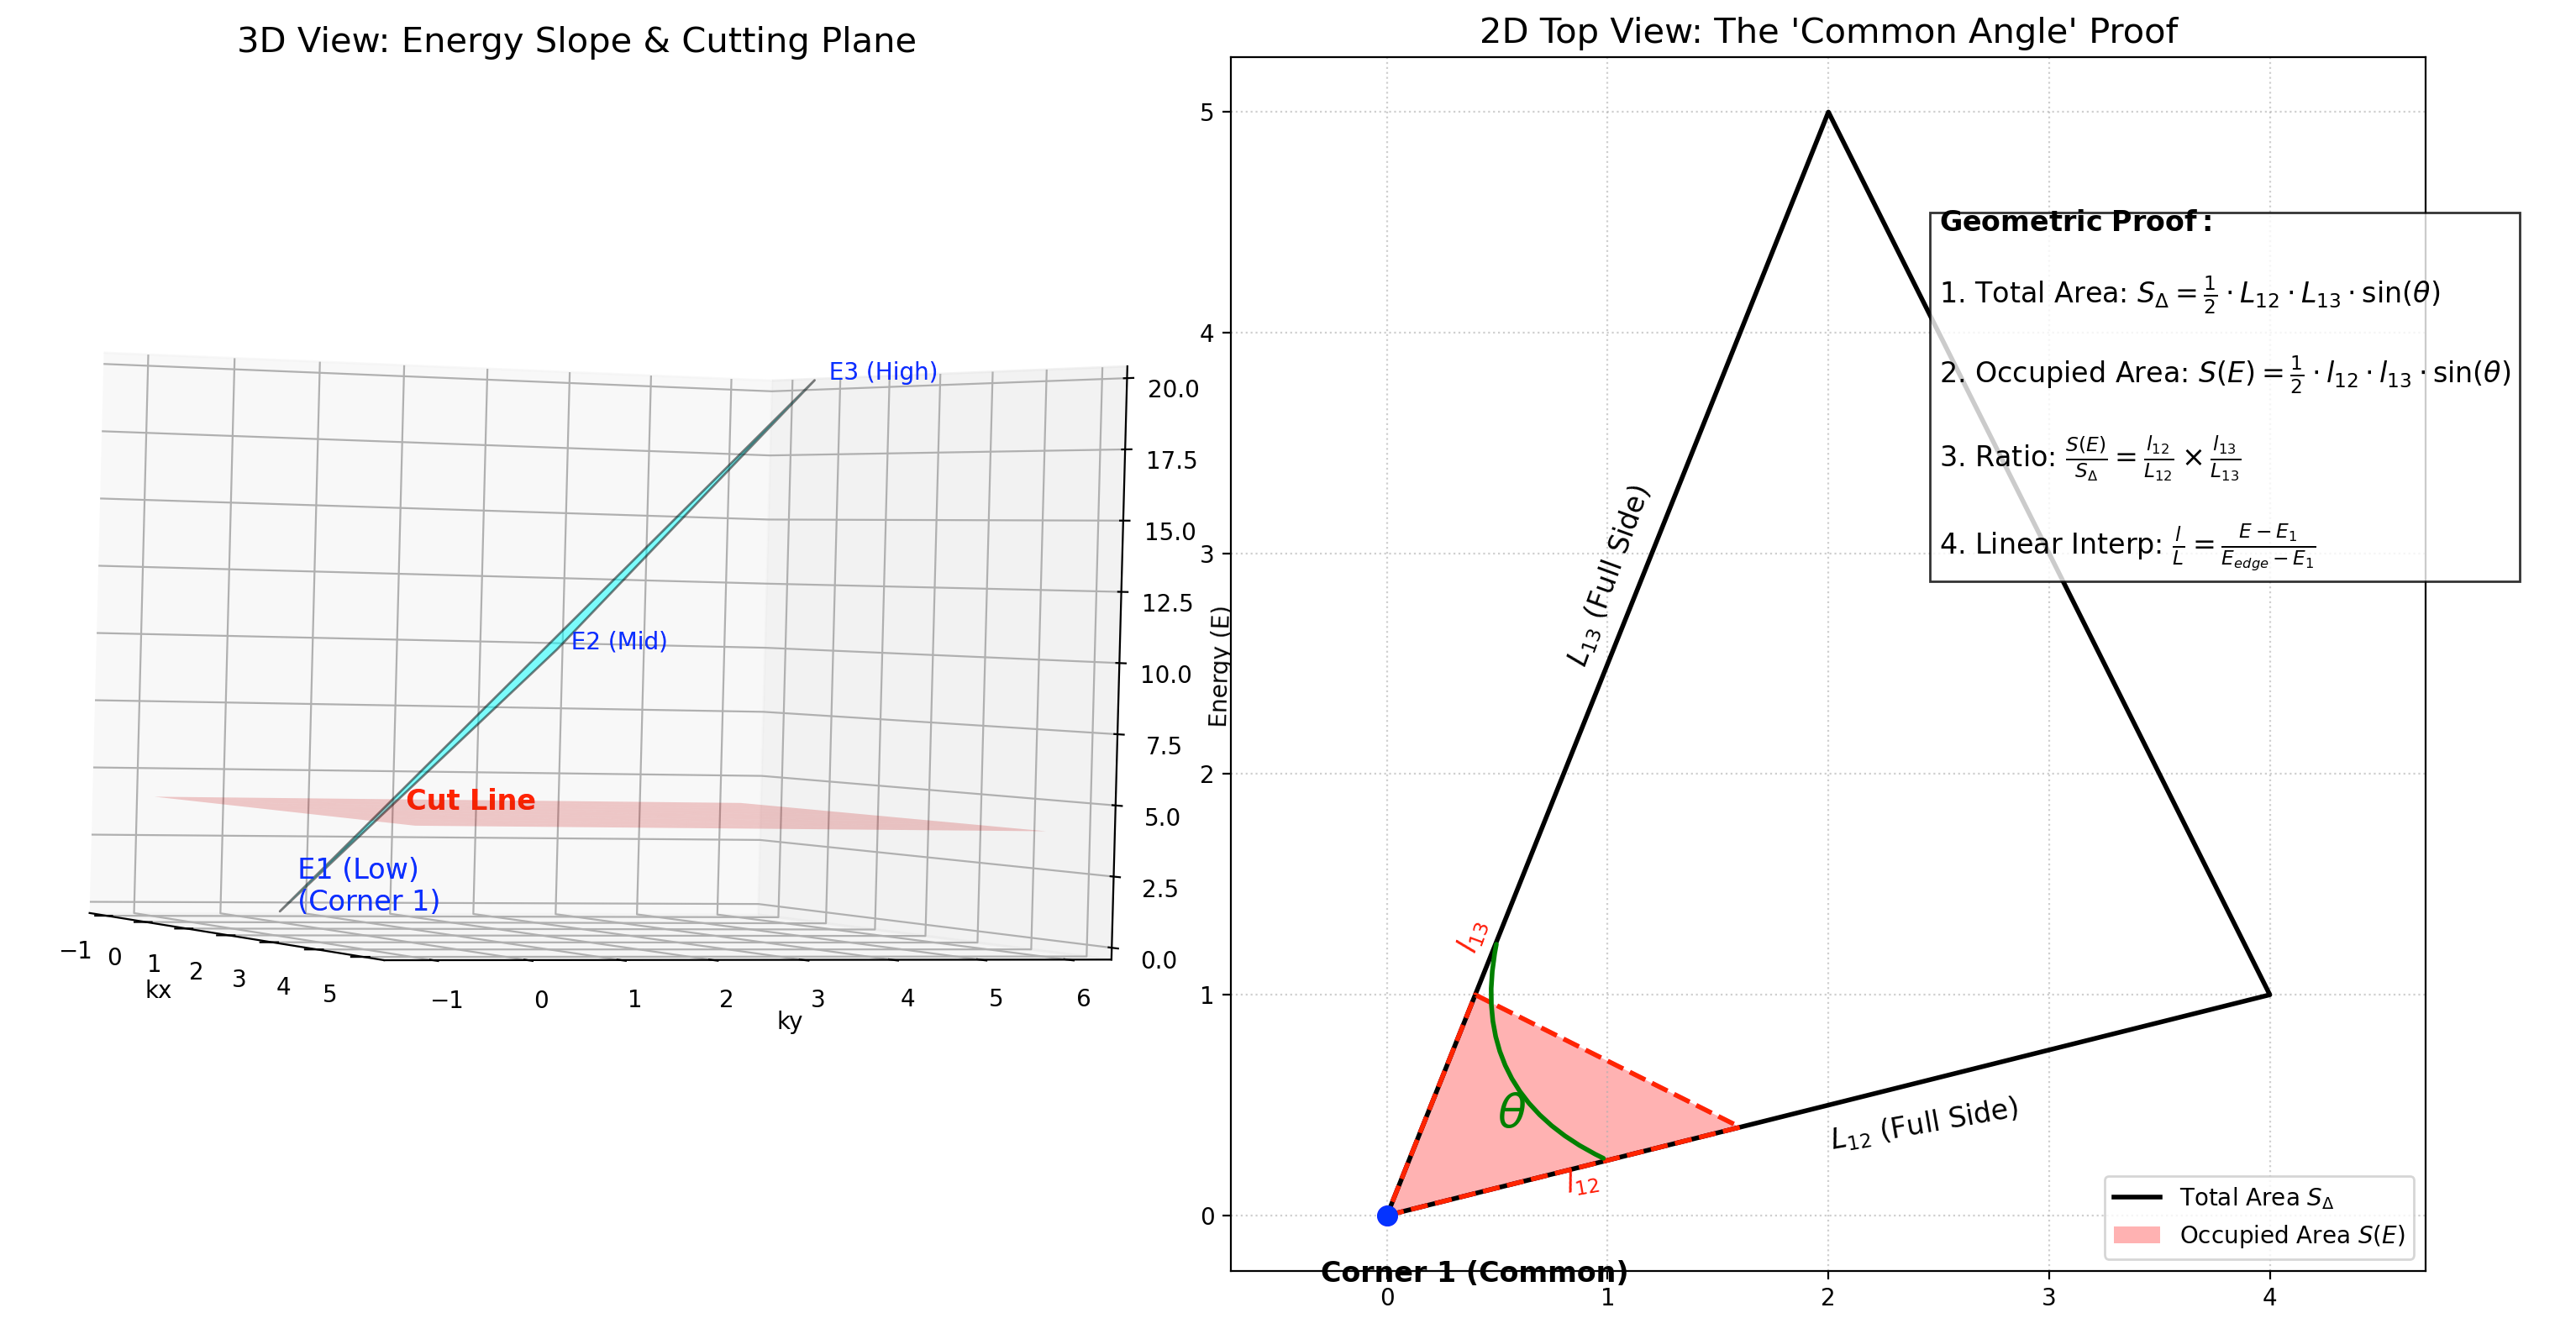
\includegraphics[width=0.8\linewidth]{pic/dos.png}
	}
	\caption{DOS for calculating the area \(S(E)\) within a triangle.}
\end{figure}


\begin{itemize}
	\item van Hove singularity
\end{itemize}

The van Hove singularity (VHS) refers to a point in the density of states (DOS) of a crystalline material where the DOS diverges or exhibits a pronounced peak. This phenomenon occurs at specific energies in the electronic band structure, typically associated with saddle points, maxima, or minima in the energy dispersion relation of electrons within the material.

For a multivariable function \(f\p{x,y}\), we have Hessen matrix
\begin{align}
	H = \begin{pmatrix}
		\frac{\partial^2 f}{\partial x^2} & \frac{\partial^2 f}{\partial x \partial y} \\
		\frac{\partial^2 f}{\partial y \partial x} & \frac{\partial^2 f}{\partial y^2}
	\end{pmatrix}
\end{align}
and we can get its eigenvalues \(\lambda_1, \lambda_2\). If \(\lambda_1, \lambda_2 < 0\) or \(\lambda_1, \lambda_2 > 0\), the point is a local maximum or minimum respectively. If \(\lambda_1 \lambda_2 < 0\), the point is a saddle point which gives rise to van Hove singularity in the DOS. In physical terms, we have the curvature matrix of the effective mass tensor 
\begin{align}
	\frac{1}{m^{*}_{ij}} = \frac{1}{\hbar^2} \frac{\partial^{2} E}{\partial k_{x} k_{y}},
\end{align}
and group velocity \(\p{v_x, v_y }= \p{\frac{\partial E}{\partial k_x}, \frac{\partial E}{\partial k_y}}\), which means at the van Hove singularity we have
\begin{align}
	\bm{v} = \bm{0}, \quad \det \bb{H} < 0.
\end{align}

\(\frac{\partial E}{\partial k_x} = \frac{\partial E}{\partial k_y} = 0\) occurs at the statiionary points which is valley bottom, band top or saddle point. At the valley bottom, band top, or the local extremum, it means the DoS band-edge cutoff which means that DOS becomes exactly zero outside the allowed energy range of the band. This drop to zero at the minimum/maximum energy of a band is called the band-edge cutoff. But what we concern is the saddle points, Because curvature has opposite signs, the DOS  yields a logarithmic divergence: \(D\p{E} \sim \ln \bv{E -E_{s}}\). In other words, the DOS diverges, but the k-space integral is still well-defined.

Near a saddle point, we can expand the energy dispersion as
\begin{align}
	E\p{k_x, k_y} = E_{s} + \alpha k^{2}_{x} - \beta k^{2}_{y},
\end{align}
and we have 
\begin{align}
	\frac{1}{\bv{\nabla E}} \sim \frac{1}{\sqrt{k^{2}_{x} + k^{2}_{y}}},
\end{align}
Thus the integral yelds 
\begin{align}
	\int \frac{d \bm{k}}{\bm{k}} \sim \ln{\bm{k}},
\end{align}
which is finite.

Numerically, we can search for the saddle points with group velocity \(v_x = v_y = 0\). The definition of group velocity is
\begin{align}
	v_{n}\p{\bm{k}} = \frac{1}{\hbar} \nabla_{\bm{k}} E_{n} \p{\bm{k}}.
\end{align}
The Feynman-Hellmann theorem gives
\begin{align}
	\frac{\partial E_{n}}{\partial \lambda} = \braket{\psi_n | \frac{\partial H}{\partial \lambda } | \psi_n}.
\end{align}
Thus, 
\begin{align}
	\begin{split}
		v_{n,x}\p{\bm{k}} & = \frac{1}{\hbar} \braket{\psi_{n, \bm{k}} \bv{\frac{\partial H \p{\bm{k}}}{\partial k_x}} | \psi_{n, \bm{k}}}, \\
		v_{n,y}\p{\bm{k}} & = \frac{1}{\hbar} \braket{\psi_{n, \bm{k}} \bv{\frac{\partial H \p{\bm{k}}}{\partial k_y}} | \psi_{n, \bm{k}}},
	\end{split}
\end{align}
substituting the Hamiltonian of BM model with heterostrain, we have
\begin{align}
	\begin{split}
		\frac{\partial H \p{\bm{k}}}{\partial k_x} & = v_F \hbar \sigma_x \\
		\frac{\partial H \p{\bm{k}}}{\partial k_y} & = v_F \hbar \sigma_y.
	\end{split}
\end{align}
Due to the particle-hole symmetry of the BM model, we just need to search the saddle points in the lower flat band.

\begin{itemize}
	\item Constructing the Hessen matrix numerically
\end{itemize}
We can use the central difference method to construct the Hessen matrix numerically, which is 
\begin{align}
	\frac{\partial v_{x}}{\partial k_x} \approx \frac{v_{x} \p{k_x + \delta} - v_{x} \p{k_x - \delta}}{2 \delta},
\end{align}
where \(\delta\) is a small step size in the momentum space. The other three elements of the Hessen matrix can be calculated similarly. The determinant of the Hessen matrix can be calculated as
\begin{align}
	\det H  = H_{{11}} H_{{22}} - H_{{12}} H_{{21}}.
\end{align}


\subsection{Numerical result}
\begin{itemize}
	\item DOS calculation
\end{itemize}
\begin{figure}
	\centering
	\subfigure[\(\epsilon = 0.01\%,\, \phi = 10^\circ\)]{
		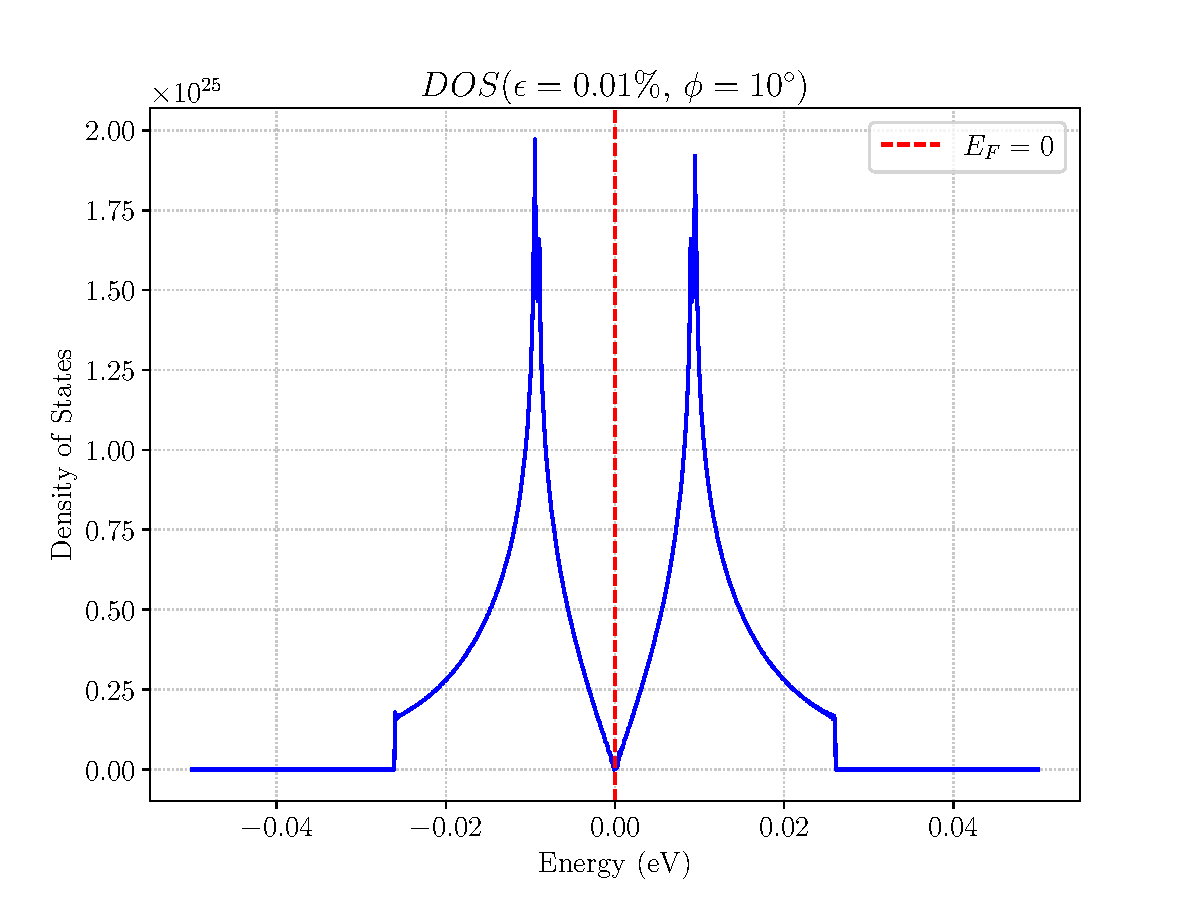
\includegraphics[width=0.35\linewidth]{pic/dos/dos_0_01.pdf}
	}
		\subfigure[\(\epsilon = 0.05\%,\, \phi = 10^\circ\)]{
		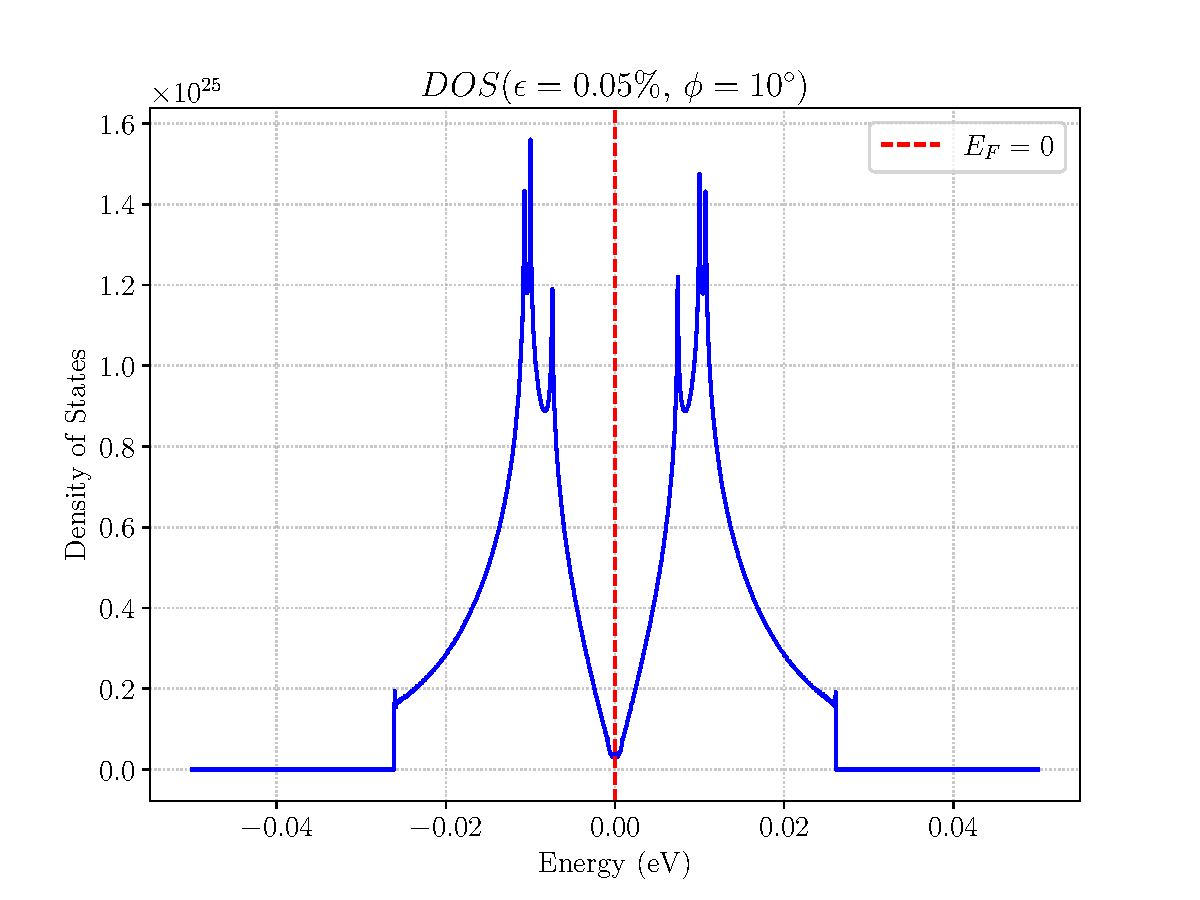
\includegraphics[width=0.35\linewidth]{pic/dos/dos_0_05.pdf}
	}
		\subfigure[\(\epsilon = 0.1\%,\, \phi = 10^\circ\)]{
		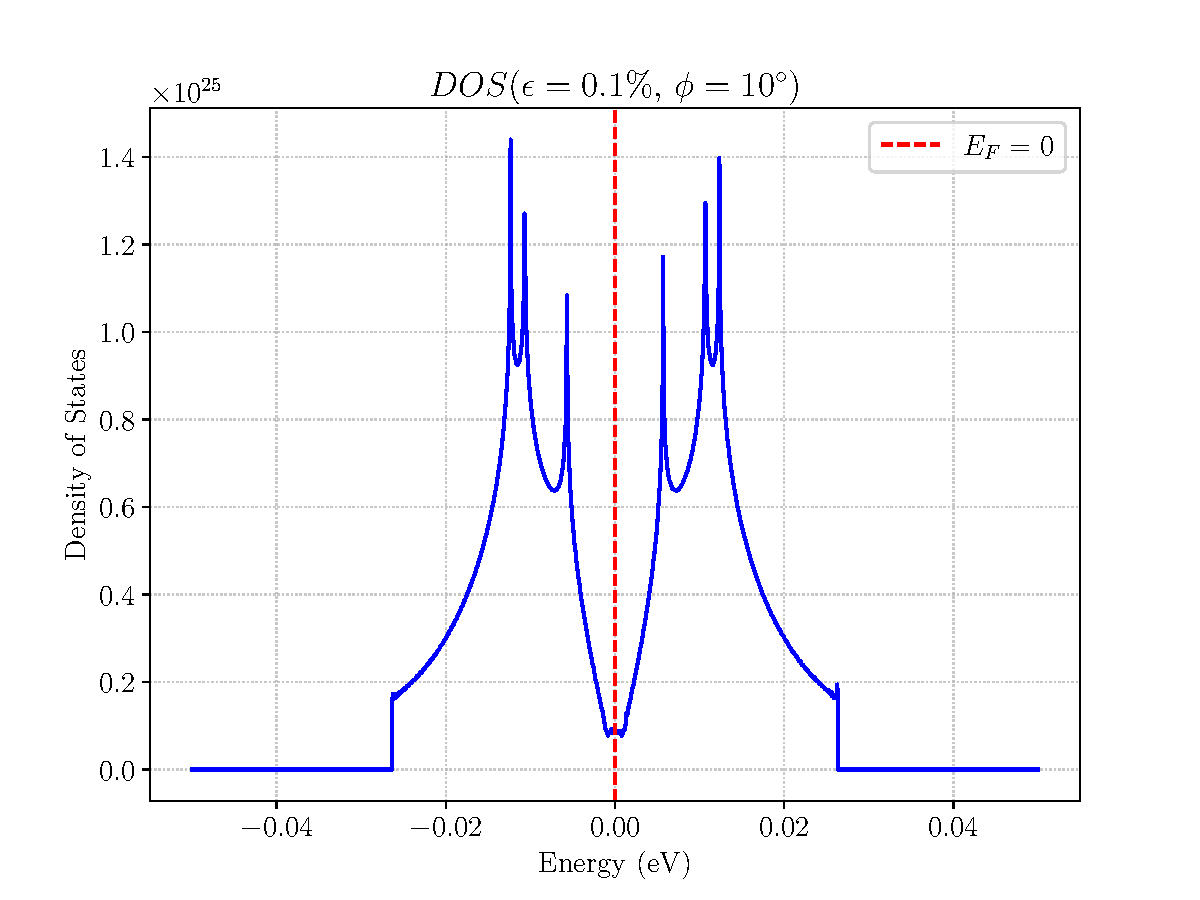
\includegraphics[width=0.35\linewidth]{pic/dos/dos_0_1.pdf}
	}
		\subfigure[\(\epsilon = 0.01\%,\, \phi = 60^\circ\)]{
		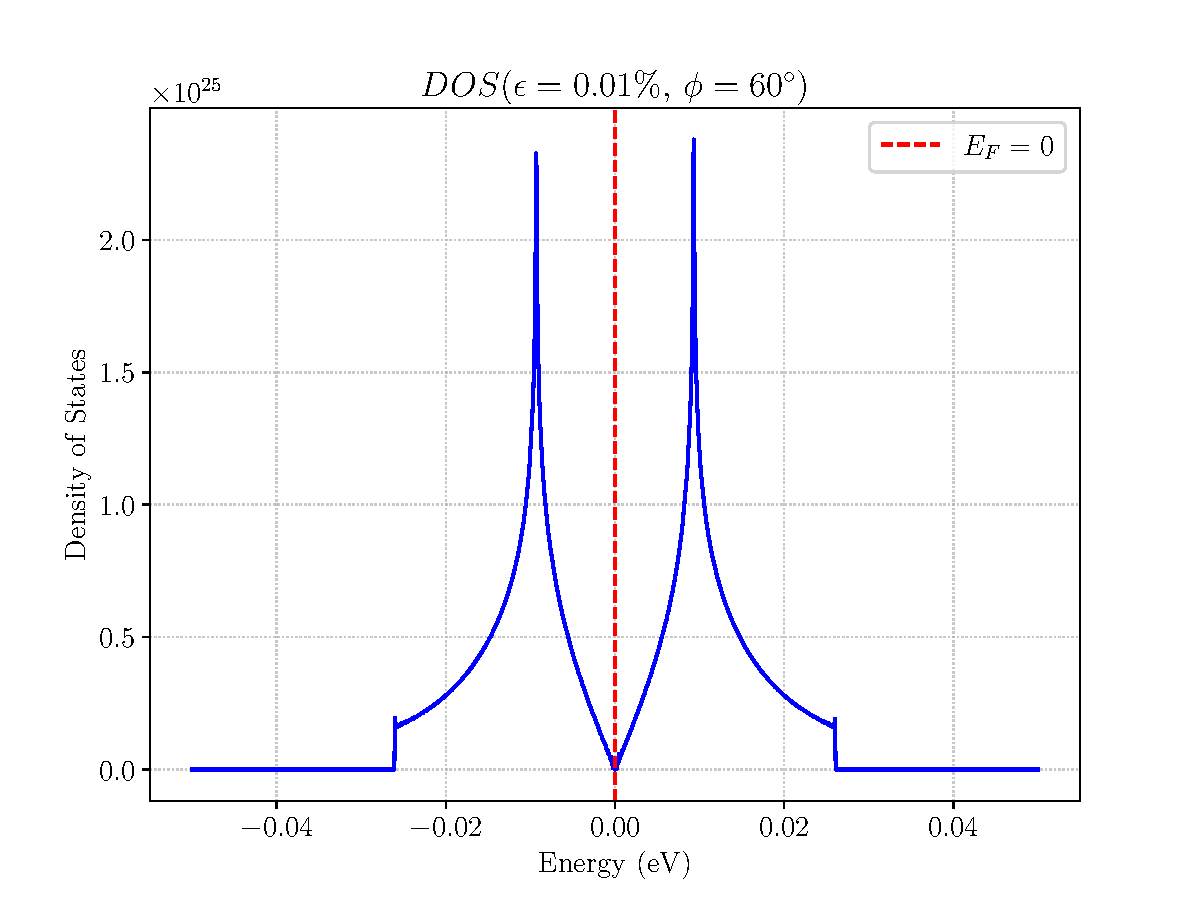
\includegraphics[width=0.35\linewidth]{pic/dos/dos_0_01_60.pdf}
	}
		\subfigure[\(\epsilon = 0.05\%,\, \phi = 60^\circ\)]{
		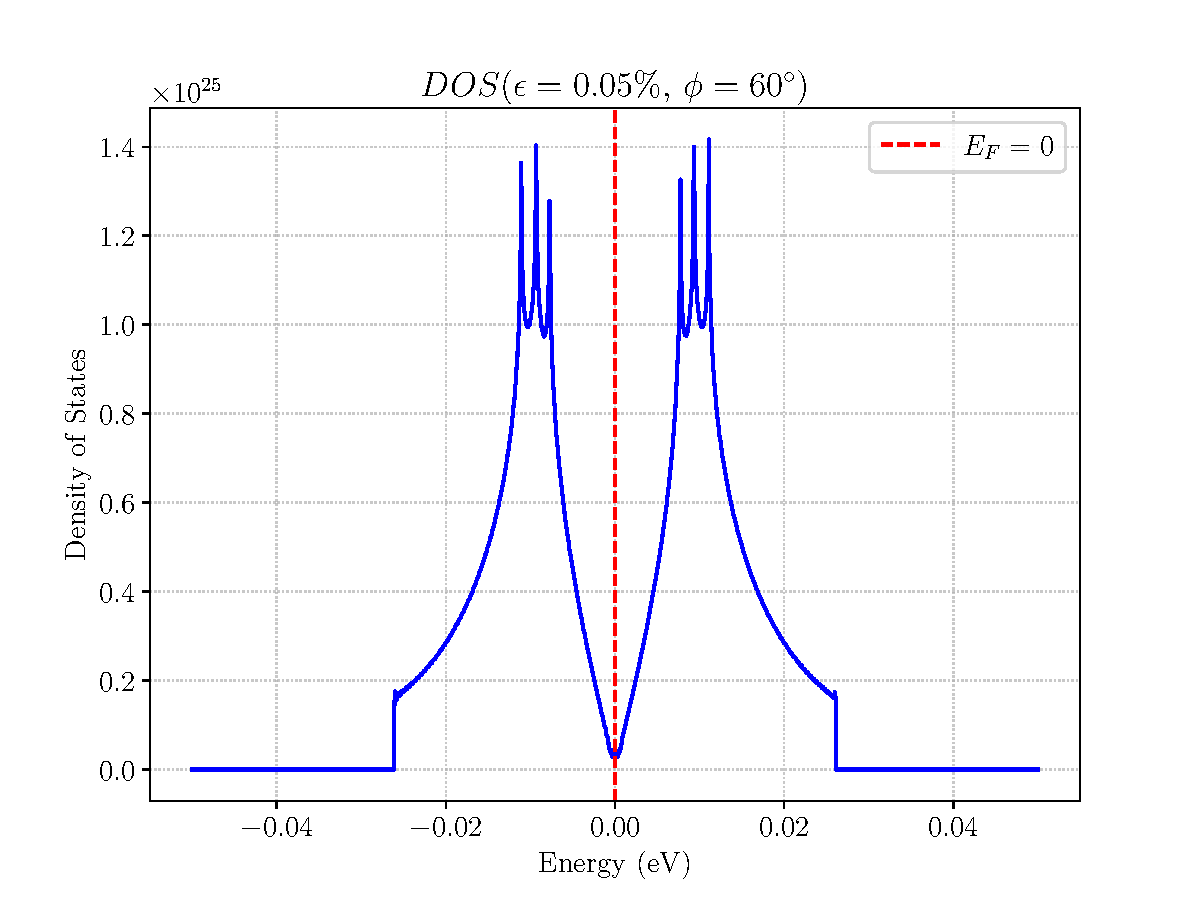
\includegraphics[width=0.35\linewidth]{pic/dos/dos_0_05_60.pdf}
	}
		\subfigure[\(\epsilon = 0.1\%,\, \phi = 60^\circ\)]{
		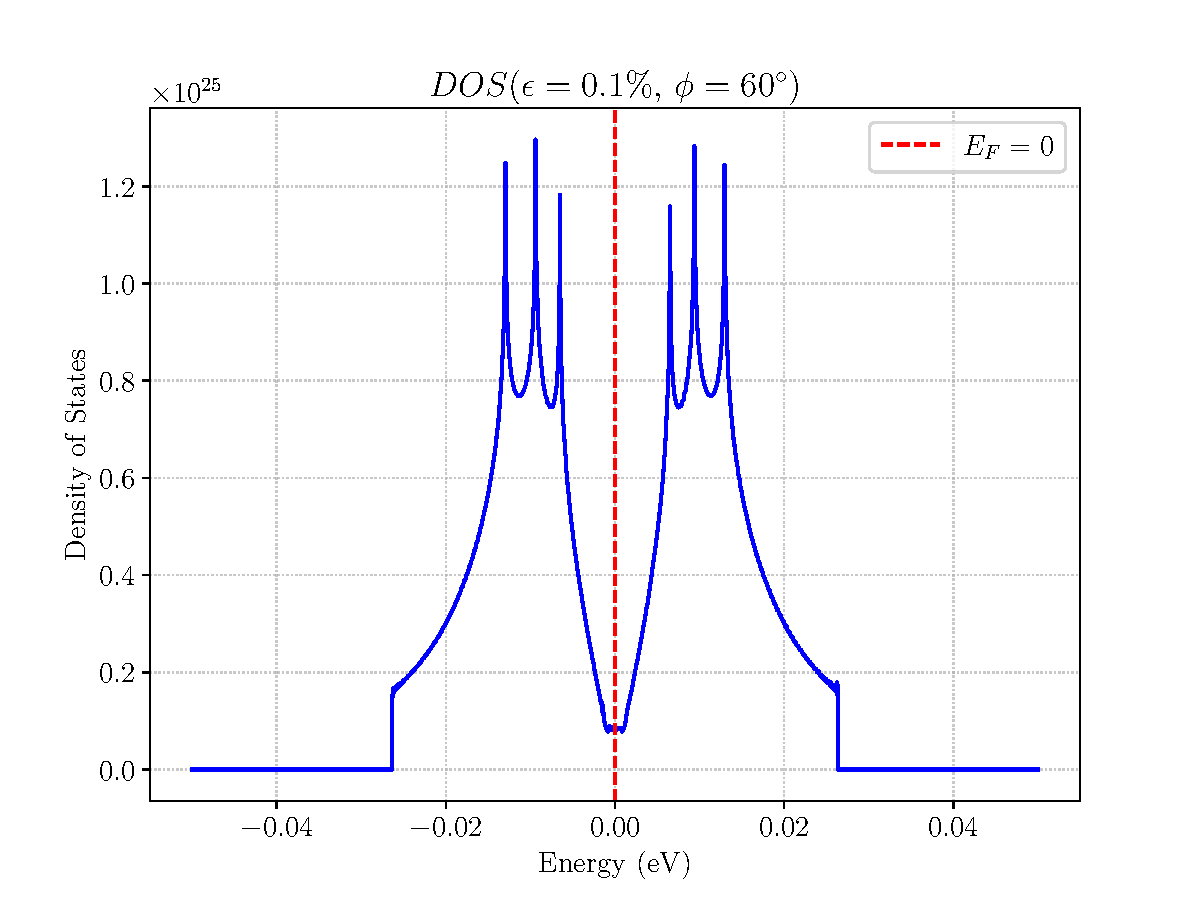
\includegraphics[width=0.35\linewidth]{pic/dos/dos_0_1_60.pdf}
	}
	\caption{DOS with different \(\epsilon\) and \(\phi\).}
\end{figure}

\begin{itemize}
	\item Distribution of Magnitude of velocity
\end{itemize}

\begin{figure}
	\centering
		\subfigure[\(\epsilon = 0.1\%,\, \phi = 60^\circ\)]{
		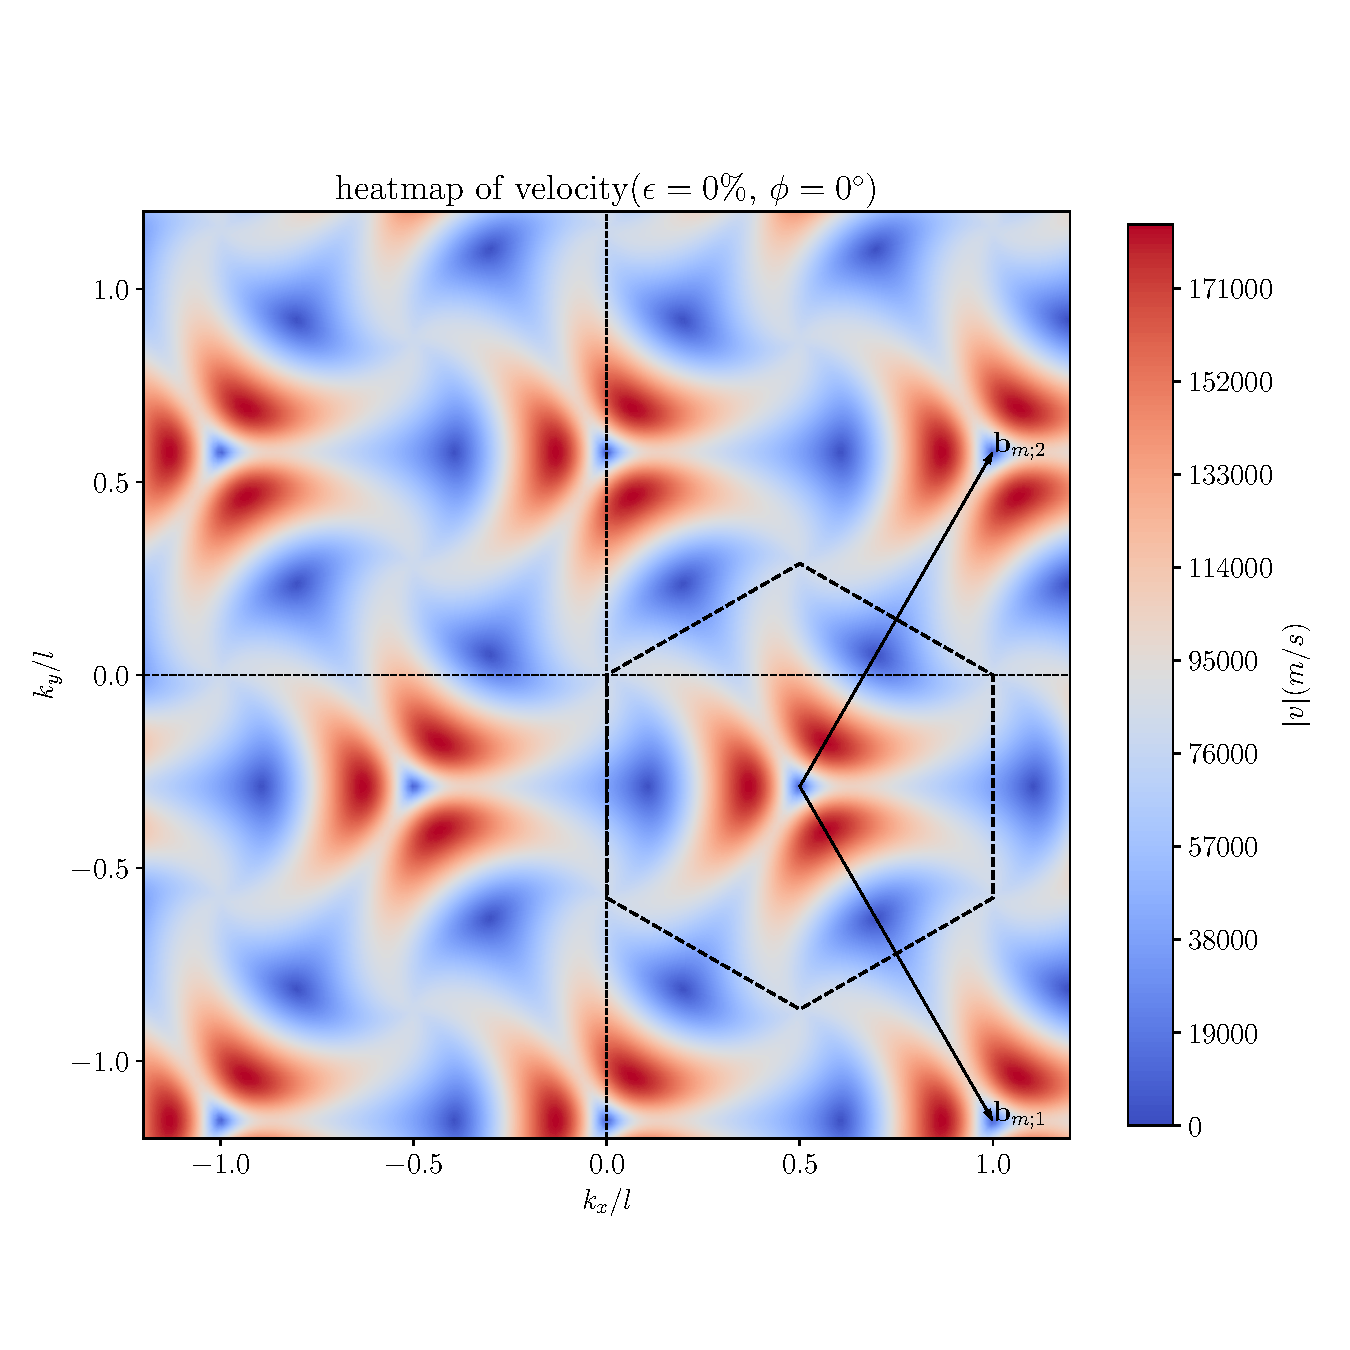
\includegraphics[width=0.35\linewidth]{pic/dis_v/config_0.pdf}
	}
	\caption{velocity distribution in moiré BZ.}
\end{figure}



\subsection{Symmetry analysis}

\begin{itemize}
	\item The number and position of vHs
\end{itemize}
With out strain, there are three vHs with same energy in the moiré Brillouin zone due to the \(C_{3z}\) symmetry. The three vHs are located at the line of \(\bm{\Gamma} - \bm{M}\). The reason why the vHs locate at this line is the \(C_{2x}\) symmetry. As we discussed before, we set \(\bm{\Gamma}\) as the rotation(symmetry) center and the line of \(\bm{\Gamma} - \bm{M}\) is the \(k_x\) axis. Due to \(C_{2x}\) symmetry, we have 
\begin{align}
	E\p{k_x, k_y} = E\p{k_x, - k_y},
\end{align}
and we differentiate both sides with respect to \(k_y\)
\begin{align}
	\begin{split}
		v_{y} \p{k_x, k_y} = \frac{\partial E\p{k_x, k_y}}{\partial k_y} & = \frac{\partial E\p{k_x, - k_y}}{\partial k_y} \\
		& = \frac{\partial E \p{k_x, - k_y}}{\partial \p{- k_y}} \cdot \frac{\partial \p{- k_y}}{\partial k_y} \\
		& = - v_{y} \p{k_x, - k_y}.
	\end{split}
\end{align}
So if we set \(k_y = 0\), we have
\begin{align}
	v_{y} \p{k_x, 0} = - v_{y} \p{k_x, 0} \Rightarrow v_{y} \p{k_x, 0} = 0.
\end{align}
Thus the vHs must locate on the line of \(\bm{\Gamma} - \bm{M}\) where \(k_y = 0\). Now we continue to prove why the vHs can not exist off the high-symmetry line. we can demonstrate it via proof by contradiction. Assuming there exists a vHs at an arbitrary position \(\bm{k}^{*} = \p{k^{*}_{x} , \delta}\) where \(\delta \neq 0\). By definition, this point must satisfy the zero-gradient condition:
\begin{align}
	\nabla E \p{k^{*}_{x} , \delta} = \bm{0}.
\end{align}
If a critial point exists at \(\bm{k}^{*}\), then due to the \(C_{2x}\) symmetry, there must be a corresponding point at \(\p{k^{*}_{x}, -\delta}\) that also satisfies the zero-gradient condition:
\begin{align}
	\nabla E \p{k^{*}_{x} , -\delta} = \bm{0}.
\end{align}
So the critial points would appear in pairs which means there are \(6\) vHs in total. However, this contradicts the known fact that there are only \(3\) vHs in the system without strain, small angle and prior to any Lifshitz transition (strictly prove can be done according to Poincaré-Hopf theorem).




\section{Fermi Surface}
\subsection{Definition}
\subsection{Primary results}
We choose two energy between the energy cross of the two vHs which are \(\phi = 40^\circ\) and \(\phi = 60^\circ\). The Fermi surface are shown below:
\begin{figure}
	\centering
		\subfigure[\(\epsilon = 0.1\%,\, \phi = 40^\circ\)]{
		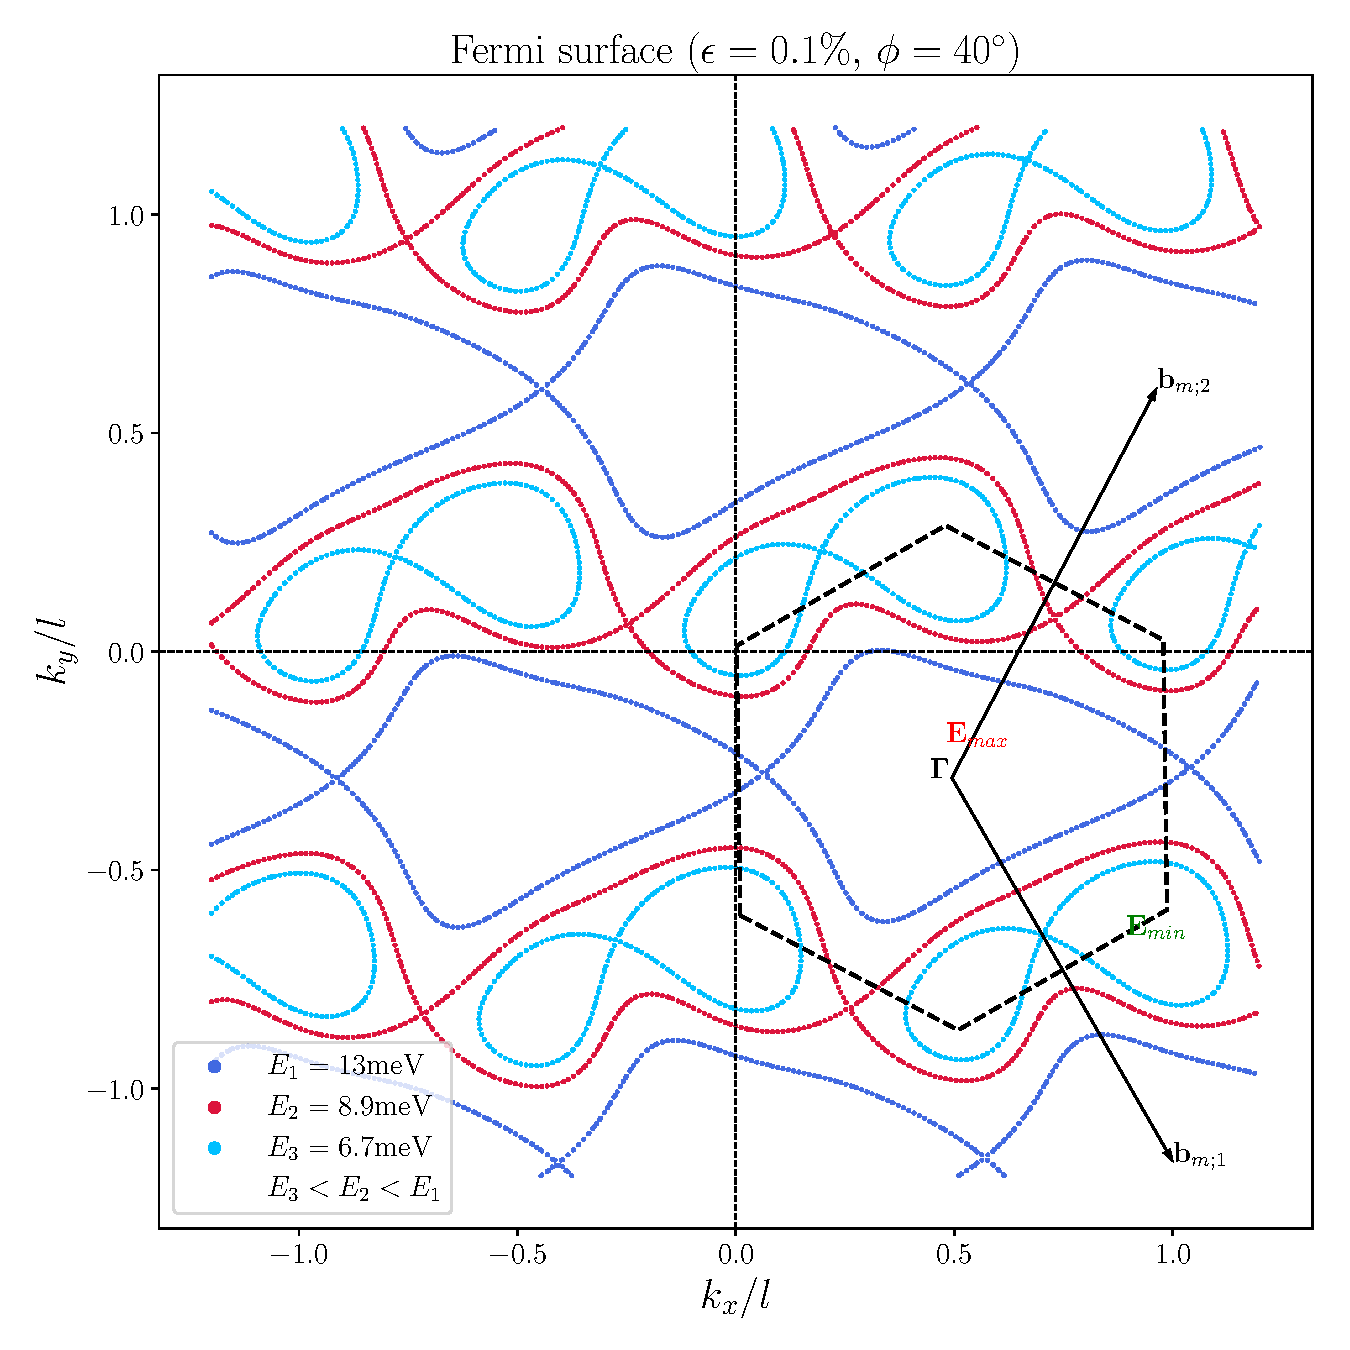
\includegraphics[width=0.35\linewidth]{pic/fs/ep_01_phi_40.pdf}
	}
		\subfigure[\(\epsilon = 0.1\%,\, \phi = 60^\circ\)]{
		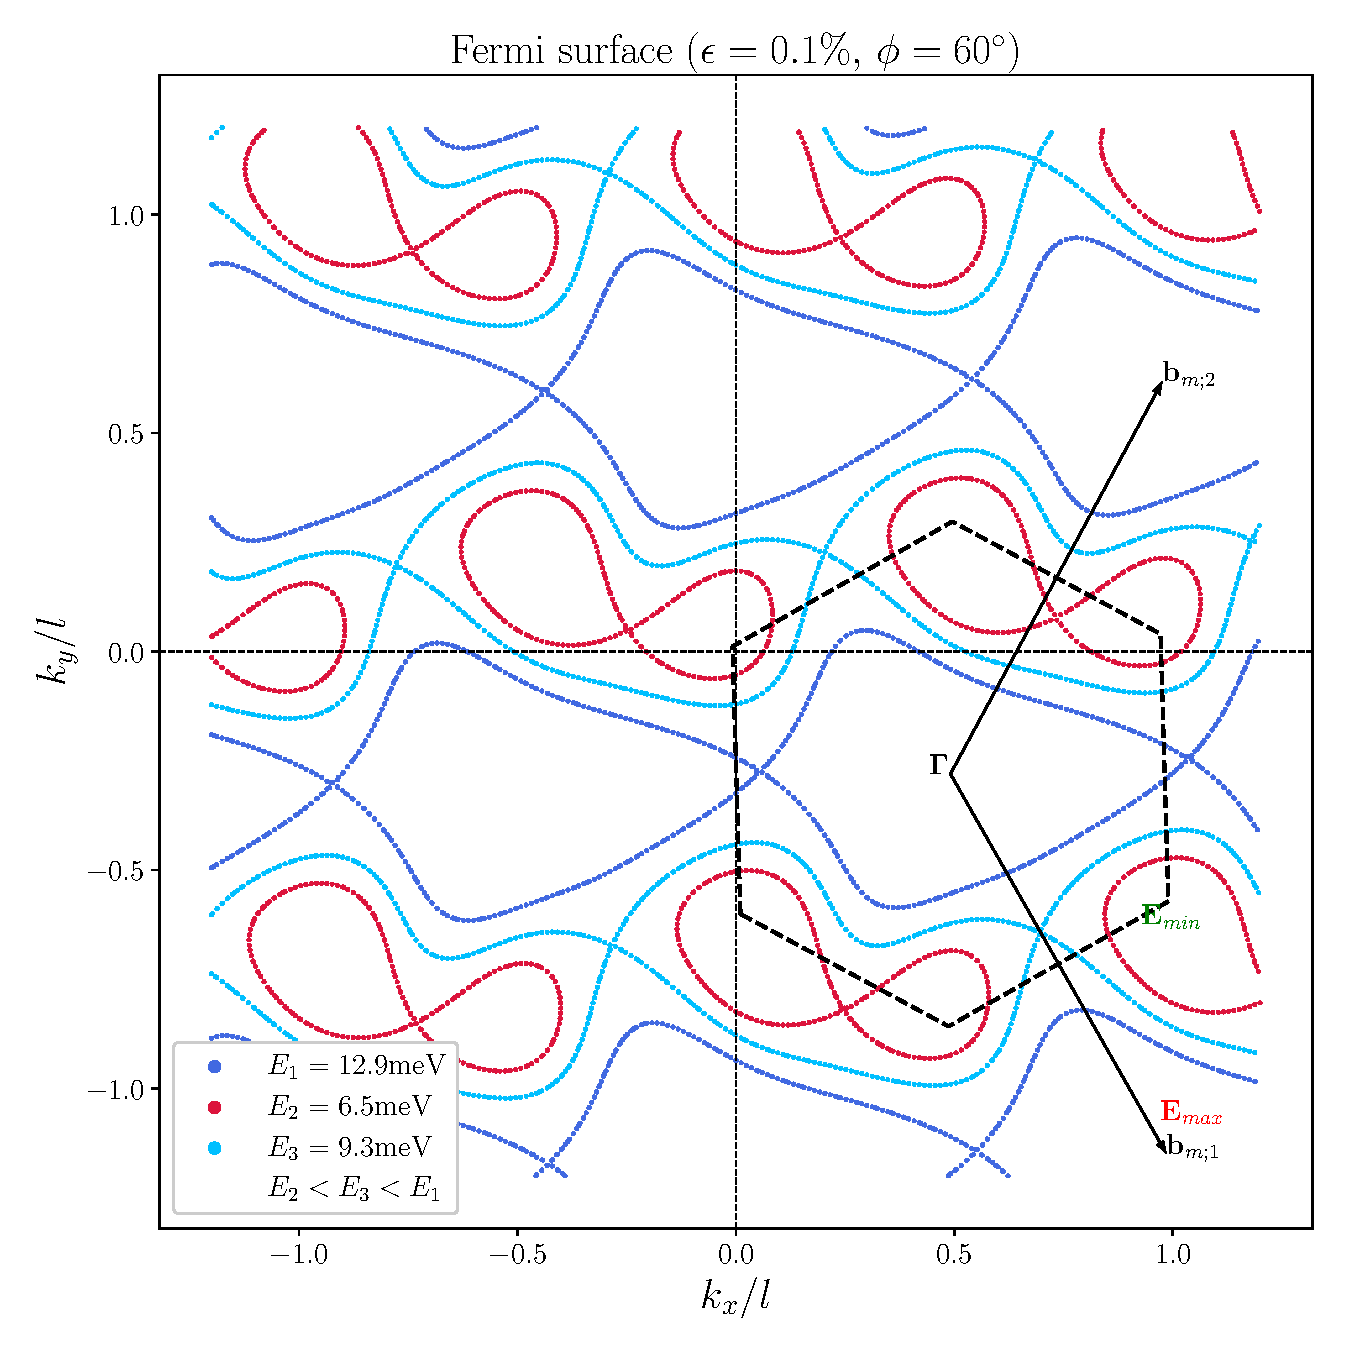
\includegraphics[width=0.35\linewidth]{pic/fs/ep_01_phi_60.pdf}
	}
\end{figure}

We can see electron pocket \(\rightarrow\) open Fermi surface  \(\rightarrow\) electron pocket \(\rightarrow\) open Fermi surface \(\rightarrow\) hole pocket with the increase of energy.


\subsection{Open Fermi surface and magnetotransport}

\section{Derivation of Pseudoscalar and Pseudovector Fields.}
The derivation begins with the continuum form of the intralayer Hamiltonian, obtained by applying the gradient expansion to the microscopic tight-binding model. The core expression involves an integration over the atomic hopping vector $\boldsymbol{y}$ and a summation over reciprocal lattice vectors $\boldsymbol{G}$ (see Eq. A2 in the paper):

\begin{equation}
H_{intra} \simeq \sum_{S,S'} \sum_{\boldsymbol{G}} e^{i\boldsymbol{G} \cdot \delta\boldsymbol{\tau}_{SS'}} \int d^2y \, e^{-i(\boldsymbol{G}+\boldsymbol{K})\cdot \boldsymbol{y}} \underbrace{e^{i \frac{\boldsymbol{y}}{2} \cdot \nabla (2\boldsymbol{U}^{||}) \cdot (\boldsymbol{G}+\boldsymbol{K})}}_{\text{Phase Factor}} t(|\boldsymbol{y}|) \left[ \Psi^\dagger \Psi + \dots \right]
\end{equation}
where $\boldsymbol{U}^{||}(\boldsymbol{x})$ is the in-plane displacement field. We focus on the lattice relaxation part $\delta \boldsymbol{U}(\boldsymbol{x})$, such that $\boldsymbol{U}^{||} \approx \boldsymbol{U}_{rot} \pm \frac{1}{2} \delta \boldsymbol{U}$.

\subsection{Step 1: Gradient Expansion of the Phase Factor}
Since the lattice relaxation $\delta \boldsymbol{U}(\boldsymbol{x})$ varies slowly on the atomic scale ($|\nabla \delta \boldsymbol{U}| \ll 1$), we expand the phase factor to the first order in gradients:

\begin{equation}
\exp\left[ i \frac{\boldsymbol{y}}{2} \cdot \nabla (\delta \boldsymbol{U}) \cdot (\boldsymbol{G}+\boldsymbol{K}) \right] \approx 1 + i \frac{y_\mu}{2} (\partial_\mu \delta U_\rho) (G+K)_\rho
\end{equation}
Here, indices $\mu, \rho \in \{x, y\}$ denote spatial components. We substitute this expansion back into the Hamiltonian and focus on the first-order correction term:

\begin{equation}
\text{Term}^{(1)}_{SS'} \propto \sum_{\boldsymbol{G}} e^{i\boldsymbol{G} \cdot \delta\boldsymbol{\tau}_{SS'}} \int d^2y \, e^{-i(\boldsymbol{G}+\boldsymbol{K})\cdot \boldsymbol{y}} t(|\boldsymbol{y}|) \left[ \frac{i}{2} y_\mu (\partial_\mu \delta U_\rho) (G+K)_\rho \right]
\end{equation}

\subsection{Step 2: Poisson Summation}
To simplify the expression, we use the property of the Fourier transform $y_\mu e^{-i\boldsymbol{q}\cdot\boldsymbol{y}} = i \frac{\partial}{\partial q_\mu} e^{-i\boldsymbol{q}\cdot\boldsymbol{y}}$ and apply the Poisson summation formula:
\begin{equation}
\sum_{\boldsymbol{G}} e^{i\boldsymbol{G}\cdot\boldsymbol{d}} \tilde{f}(\boldsymbol{G}+\boldsymbol{K}) = \sum_{\boldsymbol{R}} e^{-i\boldsymbol{K}\cdot(\boldsymbol{R}+\boldsymbol{d})} f(\boldsymbol{R}+\boldsymbol{d})
\end{equation}
Converting the momentum derivative back to real space, the integral over $\boldsymbol{y}$ transforms into a summation over real-space lattice vectors $\boldsymbol{R} = \boldsymbol{a} + \delta\boldsymbol{\tau}_{SS'}$:

\begin{equation}
\text{Term}^{(1)}_{SS'} \propto \frac{1}{2} (\partial_\mu \delta U_\rho) \sum_{\boldsymbol{R}} e^{-i\boldsymbol{K} \cdot \boldsymbol{R}} \underbrace{\partial_\rho \left[ R_\mu t(|\boldsymbol{R}|) \right]}_{\text{From } (G+K)_\rho \partial_{q_\mu}}
\end{equation}
Using the chain rule $\partial_\rho [R_\mu t(|\boldsymbol{R}|)] = \delta_{\mu\rho} t(|\boldsymbol{R}|) + R_\mu R_\rho \frac{t'(|\boldsymbol{R}|)}{|\boldsymbol{R}|}$, we arrive at the key tensor summation:

\begin{equation}
\mathcal{M}_{\mu\rho}^{SS'} = \sum_{\boldsymbol{R}} e^{-i\boldsymbol{K} \cdot \boldsymbol{R}} \left[ \delta_{\mu\rho} t(|\boldsymbol{R}|) + R_\mu R_\rho \frac{t'(|\boldsymbol{R}|)}{|\boldsymbol{R}|} \right]
\end{equation}

\subsection{Step 3: Symmetry Selection and Field Definitions}

\subsubsection{Case A: Same Sublattice ($S=S'$) $\rightarrow$ Pseudoscalar Field}
For $S=S'$, the hopping vector is $\boldsymbol{R} = \boldsymbol{a}$ (next-nearest neighbors). Due to $C_3$ symmetry:
\begin{itemize}
    \item Off-diagonal terms vanish: $\sum a_x a_y = 0$.
    \item Diagonal terms are equal: $\sum a_x^2 = \sum a_y^2$.
\end{itemize}
Thus, the tensor becomes isotropic: $a_\mu a_\rho \to \delta_{\mu\rho} \frac{1}{2} |\boldsymbol{a}|^2$. The summation yields a scalar multiple of the identity:
\begin{equation}
\mathcal{M}_{\mu\rho}^{SS} \propto \delta_{\mu\rho} \left( \frac{\mu}{2} + \alpha \right)
\end{equation}
Contracting this with the strain tensor $\partial_\mu \delta U_\rho$:
\begin{equation}
\delta_{\mu\rho} (\partial_\mu \delta U_\rho) = \partial_\mu \delta U_\mu = \nabla \cdot \delta \boldsymbol{U}
\end{equation}
\textbf{Result:} This defines the \textbf{Pseudoscalar Field} $\phi$:
\begin{equation}
\phi^{(j)} \propto \nabla \cdot \delta \boldsymbol{U}
\end{equation}

\subsubsection{Case B: Different Sublattice ($S \neq S'$) $\rightarrow$ Pseudovector Field}
For $S \neq S'$, the hopping vector is $\boldsymbol{R} = \boldsymbol{d}$ (nearest neighbors). Due to the phase factor $e^{-i\boldsymbol{K}\cdot\boldsymbol{R}}$, the sum does \textit{not} isotropize. Instead, it couples to Pauli matrices:
\begin{equation}
\mathcal{M}_{\mu\rho}^{AB} = v_F \gamma \left[ (\tau_3)_{\rho\mu} \sigma_1 + (\tau_1)_{\rho\mu} \sigma_2 \right]
\end{equation}
Contracting with $\partial_\mu \delta U_\rho$, the specific components are selected:
\begin{itemize}
    \item $\sigma_1$ couples to: $\partial_x \delta U_x - \partial_y \delta U_y$
    \item $\sigma_2$ couples to: $-(\partial_x \delta U_y + \partial_y \delta U_x)$
\end{itemize}
\textbf{Result:} These components define the \textbf{Pseudovector Field} $\mathcal{A}$:
\begin{equation}
\mathcal{A} = \begin{pmatrix} \mathcal{A}_x \\ \mathcal{A}_y \end{pmatrix} = \begin{pmatrix} \partial_x \delta U_x - \partial_y \delta U_y \\ -(\partial_x \delta U_y + \partial_y \delta U_x) \end{pmatrix}
\end{equation}
which enters the Hamiltonian as the gauge coupling $v_F \gamma \boldsymbol{\sigma} \cdot \mathcal{A}$.


\section{Dirac points and vHs Mergying}

\subsection{Symmetry analysis}
\begin{itemize}
	\item Beyond perturbation
\end{itemize}
We ask the system satisfies \(C_{2x}\) symmetry where the representation matrix of \(C_{2x}\) is \(\tau_{x} \bigotimes \sigma_{x} \), which is 
\begin{align}
	U_{C_{2x}} = \tau_{x} \otimes \sigma_{x} = \begin{pmatrix}
		0 & \sigma_{x} \\
		\sigma_{x} & 0
	\end{pmatrix}.	
\end{align}
The two Dirac points appear pairwise along the \(k_y\)axis. Due to particle-hole symmetry, they merge at the midpoint of \(\bm{q}_1\) at zero energy. So the Hamiltonian should satisfy
\begin{align}
	H(C_{2x} \bm{k}) = U_{C_{2x}} H(\bm{k}) U_{C_{2x}}^{\dagger},
\end{align}
where we can write the Bloch Hamiltonian as 
\begin{align}
	H\p{\bm{k}} = \begin{pmatrix}
		H_{t}\p{\bm{k}} & T^\dagger \\
		T & H_{b}\p{\bm{k}}
	\end{pmatrix},
\end{align}
Substituding it the commutation relation, we have
\begin{align}
	H_{t/b}\p{C_{2x}\bm{k}} = \sigma_{x} H_{b/t}\p{\bm{k}} \sigma_{x}.
\end{align}
To satisfy the \(C_{2x}\) symmetry, we need rewrite the Hamiltonian as the symmetric form where the origin set as \(\bm{\Gamma}_{m}\)
\begin{align}
	\begin{split}
		H_{t}\p{\bm{k}} & = v_{F} \hbar \bb{\bm{k} - \bm{Q}_{t}} \cdot \bm{\sigma} + \alpha \vph \mathbb{I} + v_{F} \gamma \bm{A} \cdot \bm{\sigma} \\
		H_{b}\p{\bm{k}} & = v_{F} \hbar \bb{\bm{k} - \bm{Q}_{b}} \cdot \bm{\sigma} - \alpha \vph \mathbb{I} - v_{F} \gamma \bm{A} \cdot \bm{\sigma},
	\end{split}
\end{align}
where geometry asks 
\begin{align}
		\bm{Q}_{t}  = \bm{K}_{t} - \bm{\Gamma}_{m}, \quad \bm{Q}_{b} = \bm{K}_{b} - \bm{\Gamma}_{m}.
\end{align}
For the scalar term, 
\begin{align}
	- \alpha \vph \mathbb{I} = \sigma_{x} \alpha \vph \mathbb{I} \sigma_{x},
\end{align}
which leads to 
\begin{align}
	\vph = 0 \Leftrightarrow \epsilon_{1} = - \epsilon_{2} \Leftrightarrow \nu = 1.
\end{align}
and the vector term 
\begin{align}
	- v_{F} \gamma \p{A_{x} \hat{\sigma}_{x} + A_{y} \hat{\sigma}_{y}} = v_{F} \gamma \p{A_{x} \hat{\sigma}_{x} - A_{y} \hat{\sigma}_{y}},
\end{align}
and we get
\begin{align}
	A_{x} = 0 \Leftrightarrow \cos{2 \te} = 0 \Leftrightarrow \te = \p{\frac{n}{2}+ \frac{1}{4}} \pi,
\end{align}
which means the direction of principle axes of strain is along the \(k_y\) axis. Also the momentum term is naturally satisfied the commutation relation.

The determining the appropriate value of \(\epsilon\) can be achieved by solving the equation \(E \p{\bm{q}_{1}/2} = 0\) which is hard for analytical solving.

\subsection{Numerical results}

Here we give some numerical results about the configuration of gap which indicates the position of Dirac points when \(\phi = 45^\circ\). 

\begin{figure}
	\centering
		\subfigure[\(\epsilon = 0.01\%\)]{
		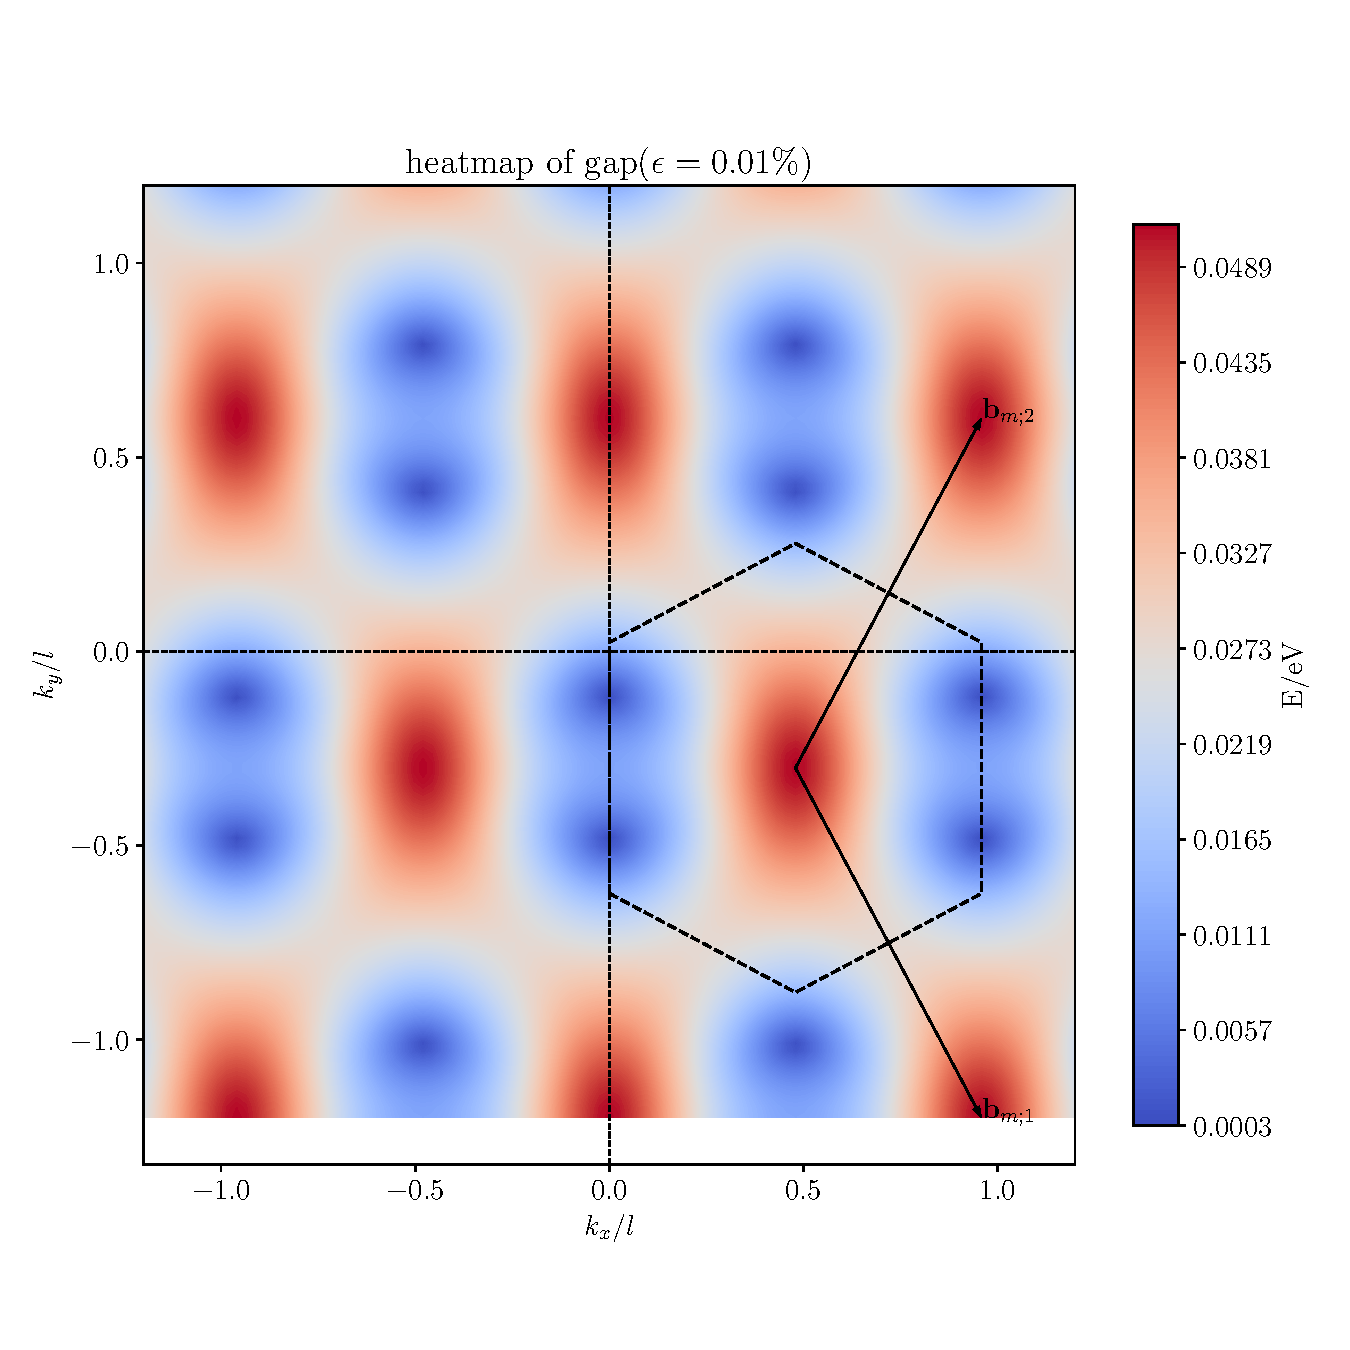
\includegraphics[width=0.45\linewidth]{pic/mergy/gap_ep_001.pdf}
	}
		\subfigure[\(\epsilon = 0.25\)]{
		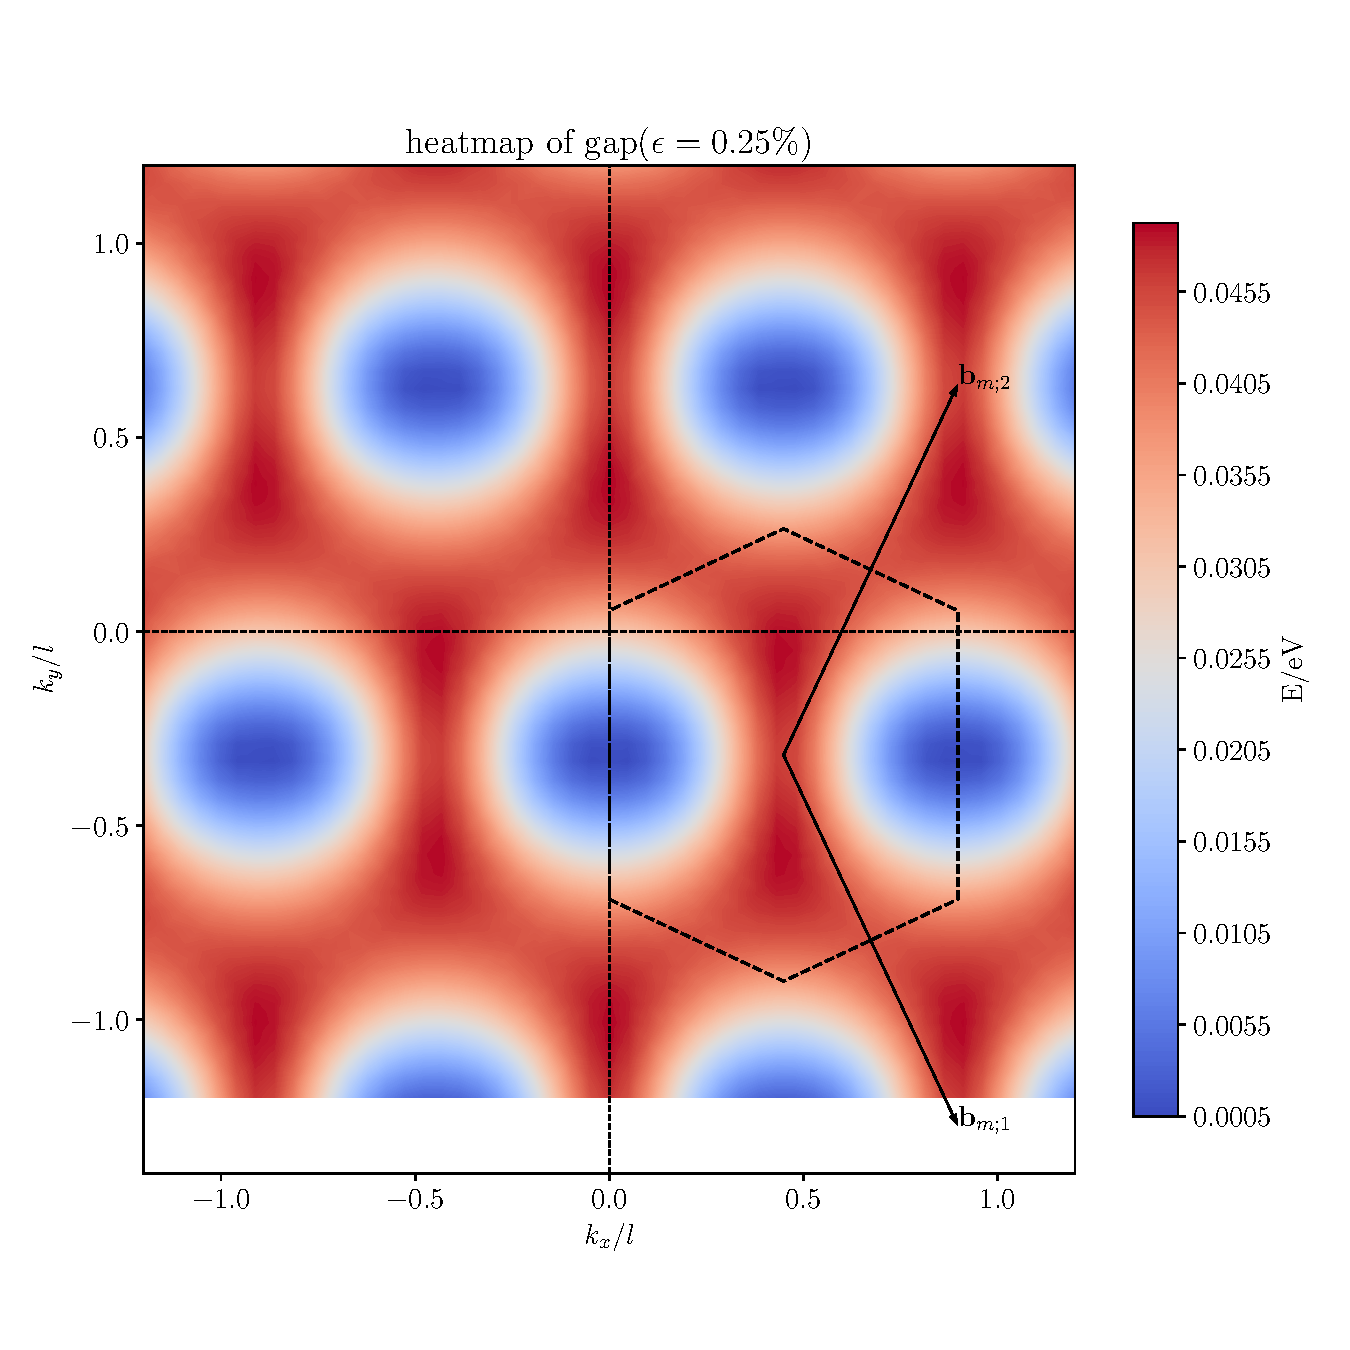
\includegraphics[width=0.45\linewidth]{pic/mergy/gap_ep_025.pdf}
	}
		\subfigure[\(\epsilon = 0.3\%\)]{
		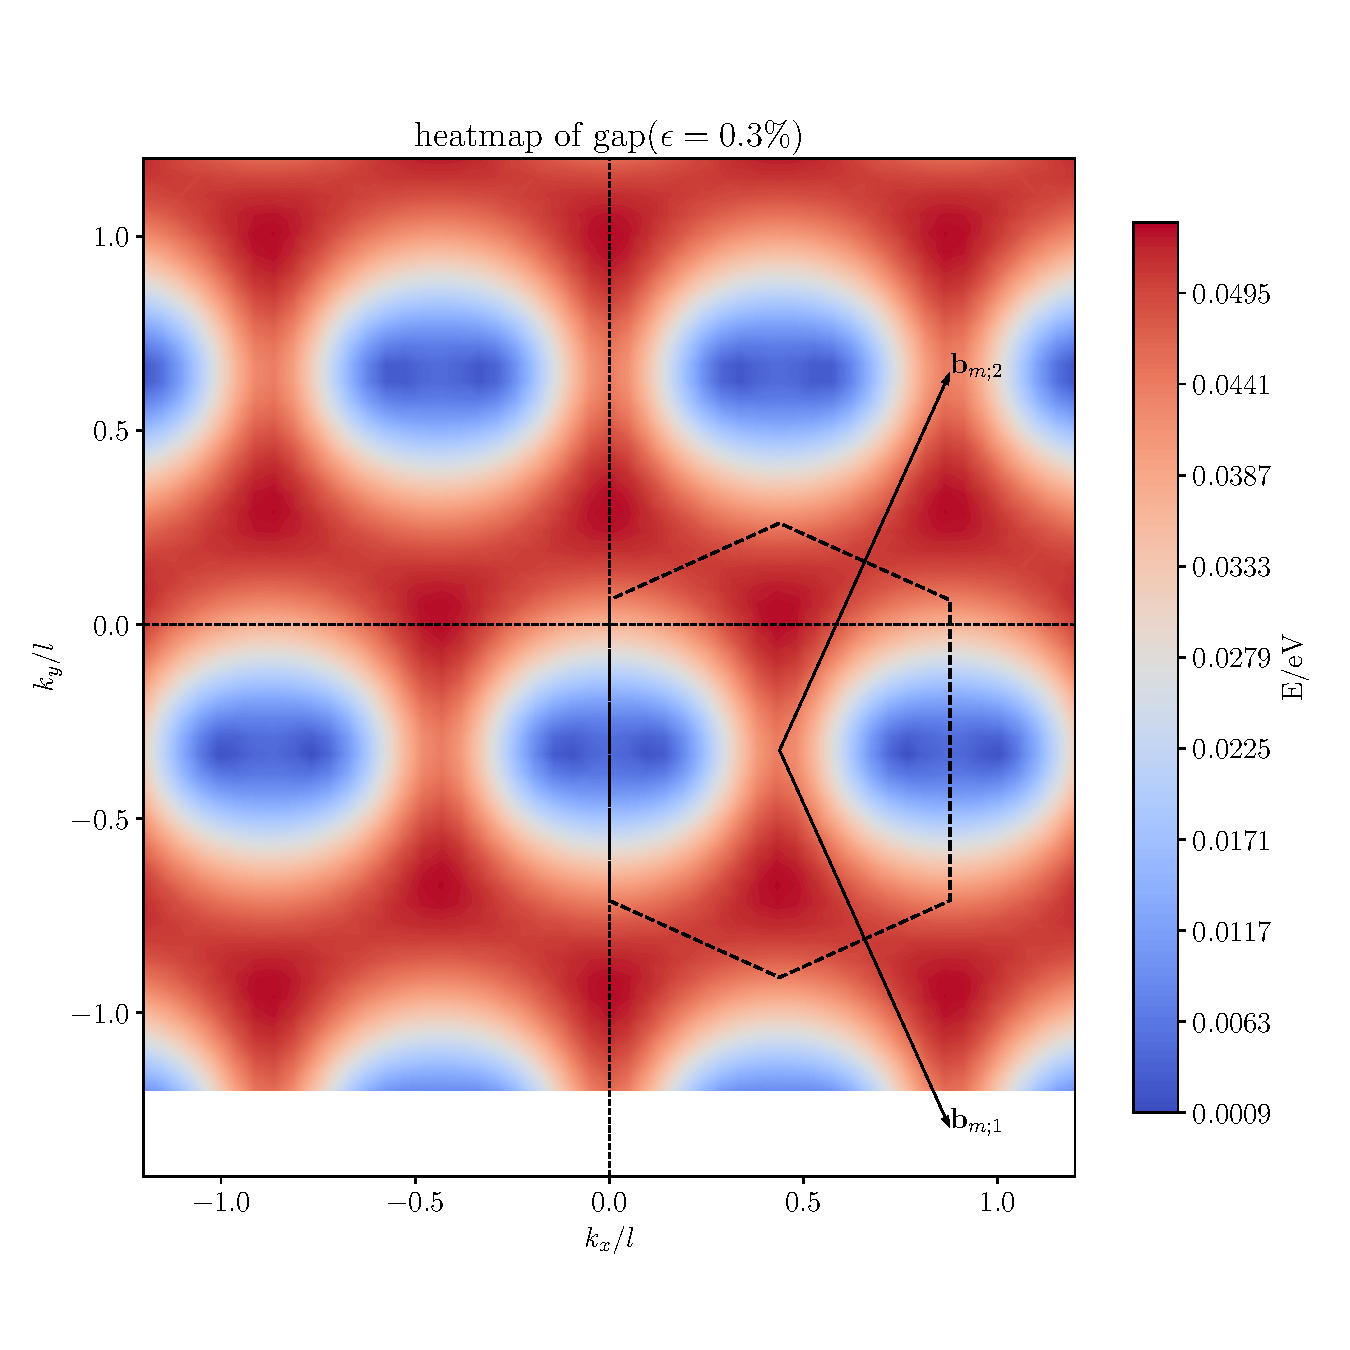
\includegraphics[width=0.45\linewidth]{pic/mergy/gap_ep_03.pdf}
	}
		\subfigure[\(\epsilon = 0.8\%\)]{
		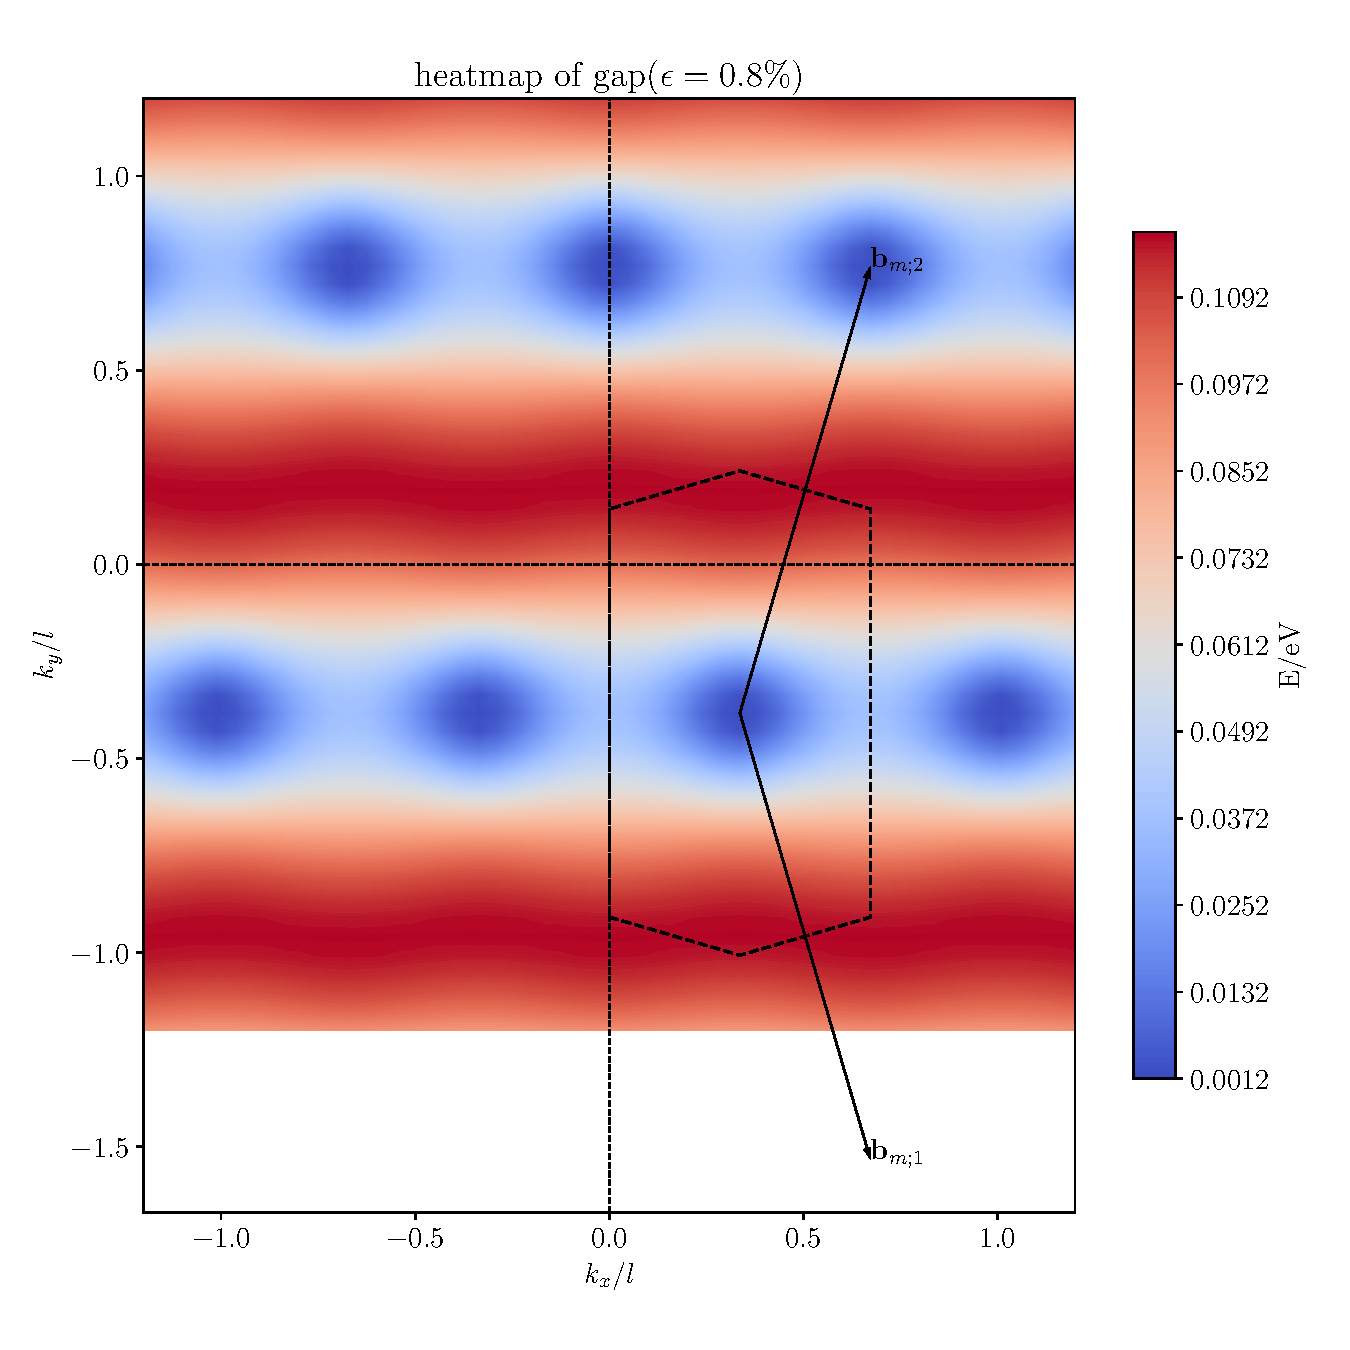
\includegraphics[width=0.45\linewidth]{pic/mergy/gap_ep_08.pdf}
	}
\end{figure}

We can see \(\epsilon\) arises from \(0.01\% \rightarrow 0.24\%\), the two Dirac points first move longitudinally along the \(k_y\) axis and then merge at the midpoint of \(\bm{q}_1\) during \(\epsilon\) within  \( 0.24\% \sim 0.27 \%\).  

However,  as \(\epsilon\) continues to increase, the two Dirac points begin to move transversely. We can see the two Dirac points apart at \(\epsilon = 0.3\%\). With further increase in \(\epsilon\), they merge agian at the \(\bm{\Gamma}\) point.

\textcolor{red}{
	Question: 1. Why does the increase of \(\epsilon\) cause the Dirac points to move in two different direction? \\
	2. Why does the two Dirac points keep merging?
}


\end{document}






